%   DOCUMENT CLASS  %%%%%%%%%%%%%%%%%%%%%%%%%%%%%%%%%%%%%%%%%%%%%%%%%%%%%%%%%%%
%
%   Use the `sfuthesis` class to format your thesis. If your program does not
%   require a thesis defence, use the class option `undefended` like so:
%
%     \documentclass[undefended]{sfuthesis}
%
%   To generate a signature page for your defence, use the `sfuapproval` class
%   instead, by replacing the below line with
%
%     \documentclass{sfuapproval}
%
%   For more information about thesis formatting requirements, go to
%
%     http://www.lib.sfu.ca/help/publish/thesis
%
%   or ask a thesis advisor at the SFU Research Commons.
%
%\documentclass{sfuapproval}
\documentclass{sfuthesis}



%   DOCUMENT METADATA  %%%%%%%%%%%%%%%%%%%%%%%%%%%%%%%%%%%%%%%%%%%%%%%%%%%%%%%%
%
%   Fill in the following information for the title page and approval page.
%

\title{Quantifying Inter-generational Equity under Different Target Benefit Plan Designs}
\thesistype{Project}
\author{Lu Yi}
\previousdegrees{%
	B.Sc., Simon Fraser University, 2015}
\degree{Master of Science}
\discipline{Statistics and Actuarial Science}
\department{Department of Statistics and Actuarial Science}
\faculty{Faculty of Science}
\copyrightyear{2018}
\semester{Summer 2018}
\date{June 20, 2018}

\keywords{Target Benefit Plans; Inter-generational Equity; Asset Liability Management; Economic Scenario Generator; Multivariate Time Series; Stochastic Simulation; Risk-Neutral Pricing}

\committee{%
	\chair{Jinko Graham}{Professor}
	\member{Ms. Barbara Sanders}{Senior Supervisor\\Associate Professor}
	\member{Dr. Jean-Fran\c cois B\' egin}{Co-Supervisor\\Assistant Professor}
	\member{Dr. Gary Parker}{Internal Examiner\\Associate Professor}
}



%   PACKAGES %%%%%%%%%%%%%%%%%%%%%%%%%%%%%%%%%%%%%%%%%%%%%%%%%%%%%%%%%%%%%%%%%%
%
%   Add any packages you need for your thesis here.
%   You don't need to call the following packages, which are already called in
%   the sfuthesis class file:
%
%   - appendix
%   - etoolbox
%   - fontenc
%   - geometry
%   - lmodern
%   - nowidow
%   - setspace
%   - tocloft
%
%   If you call one of the above packages (or one of their dependencies) with
%   options, you may get a "Option clash" LaTeX error. If you get this error,
%   you can fix it by removing your copy of \usepackage and passing the options
%   you need by adding
%
%       \PassOptionsToPackage{<options>}{<package>}
%
%   before \documentclass{sfuthesis}.
%
%   The following packages are a few suggestions you might find useful.
%
%   (1) amsmath and amssymb are essential if you have math in your thesis;
%       they provide useful commands like ``blackboard bold'' symbols and
%       environments for aligning equations.
%   (2) amsthm includes allows you to easily change the style and numbering of
%       theorems. It also provides an environment for proofs.
%   (3) graphicx allows you to add images with \includegraphics{filename}.
%   (4) hyperref turns your citations and cross-references into clickable
%       links, and adds metadata to the compiled PDF.
%   (5) pdfpages lets you import pages of external PDFs using the command
%       \includepdf{filename}. You will need to do this if your research
%       requires an Ethics Statement.
%

\usepackage{amsmath}                            % (1)
\usepackage{amssymb}                            % (1)
\usepackage{amsthm}                             % (2)
\usepackage{graphicx}                           % (3)
\usepackage[pdfborder={0 0 0}]{hyperref}        
\usepackage{pdfpages}                         % (5)




% ...
% ...
% ...
% ... add your own packages here!

\usepackage{multirow}
\usepackage{graphicx}
\usepackage{caption}
\usepackage{subcaption}
\usepackage{actuarialangle}
\usepackage{amssymb}
\usepackage{mathtools}
\usepackage{actu}
\usepackage[utf8]{inputenc}
\usepackage[english]{babel}
\usepackage[document]{ragged2e}
\usepackage{booktabs}
\usepackage{array}
\usepackage{arydshln}
\usepackage{dcolumn}
\usepackage{float}
\usepackage{natbib}
\usepackage{CJKutf8}
\usepackage{scrextend}
\deffootnote[1em]{1em}{1em}{\textsuperscript{\thefootnotemark}\,}
\usepackage{chngcntr}
\counterwithout{footnote}{chapter}


\DeclareMathOperator{\E}{\mathbb{E}}
\numberwithin{equation}{chapter}
\usepackage{chngcntr}
\counterwithin{table}{chapter}
\counterwithin{figure}{chapter}

\mathtoolsset{showonlyrefs}

%\captionsetup[table]{ singlelinecheck=off} 
\captionsetup{labelfont={bf,small}, textfont={small}, justification=justified, singlelinecheck=off} %singlelinecheck=false
%\newcommand\mycaption[2]{\caption{\textbf{#1}\newline\small#2}}
%\usepackage[capitalise, noabbrev]{cleveref}
%\usepackage{autonum}

%   OTHER CUSTOMIZATIONS %%%%%%%%%%%%%%%%%%%%%%%%%%%%%%%%%%%%%%%%%%%%%%%%%%%%%%
%
%   Add any packages you need for your thesis here. We've started you off with
%   a few suggestions.
%
%   (1) Use a single word space between sentences. If you disable this, you
%       will have to manually control spacing around abbreviations.
%   (2) Correct the capitalization of "Chapter" and "Section" if you use the
%       \autoref macro from the `hyperref` package.
%   (3) The LaTeX thesis template defaults to one-and-a-half line spacing. If
%       your supervisor prefers double-spacing, you can redefine the
%       \defaultspacing command.
%

\frenchspacing                                    % (1)
\renewcommand*{\chapterautorefname}{Chapter}      % (2)
\renewcommand*{\sectionautorefname}{Section}      % (2)
\renewcommand*{\subsectionautorefname}{Section}   % (2)
% \renewcommand{\defaultspacing}{\doublespacing}  % (3)
% ...
% ...
% ...
% ... add your own customizations here!




%   FRONTMATTER  %%%%%%%%%%%%%%%%%%%%%%%%%%%%%%%%%%%%%%%%%%%%%%%%%%%%%%%%%%%%%%
%
%   Title page, committee page, copyright declaration, abstract,
%   dedication, acknowledgements, table of contents, etc.
%
%   If your research requires an Ethics Statement, download one from the
%   SFU library website and uncomment the appropriate lines below.
%

\begin{document}
	
	\frontmatter
	\maketitle{}
	\makecommittee{}
	
	%\addtoToC{Ethics Statement}%
	%\includepdf[pagecommand={\thispagestyle{plain}}]{ethicsstatement.pdf}%
	%\clearpage
	
	\begin{abstract}
		\justify
		In this research, we investigate the value of inter-generational transfers under various target benefit plan designs. The contingent retirement benefits are decomposed into embedded options, and the risk-adjusted values of these options are calculated and compared across generations. For this purpose, an economic scenario generator is implemented: the economic variables’ dynamics are generated by a model that combines the first-order vector autoregressive model and the generalized autoregressive conditional heteroscedasticity process. A corresponding risk-neutral model is derived and estimated using the prices of financial assets; the latter is helpful to price the embedded options. 
		
		\justify
		We study four target benefit plans with different design elements. We find that inter-generational value transfers arise by simply joining the collective pension scheme even without the inclusion of any intertemporal benefit smoothing designs. Without additional source of funding, we show that benefit security and stability can be achieved by adopting plan designs that allow temporary inter-generational subsidization, e.g., plan designs with no-action range. We show that adding a symmetric no-action range can reduce the volatility of retirement benefits without triggering significant value transfers, at least under the assumption of stationary demographic profile and when the simulation of economic scenarios starts from its long-term equilibrium level.
	\end{abstract}
	
	
	\begin{dedication}
		To my \begin{CJK*}{UTF8}{gbsn}外婆, 爸爸妈妈\end{CJK*} and my beloved husband! 
	\end{dedication}
	
	
	\begin{acknowledgements}

		\justify
		I would like to start by thanking my senior supervisor Professor Barbara Sanders, for her constant constructive feedback on my research, for being my main source of knowledge in actuarial science (through four courses), for starting me on the path of research in a summer, for taking me on as her student and providing interesting projects in pension studies that led to my first conference experience, and for all her generous encouragement and guidance during both of my undergraduate and graduate studies. She is, without question, a great supervisor to work with.

		

		\justify
		I want to thank my co-supervisor Professor Jean-François Bégin, for being such a knowledgeable, inspiring, and responsive mentor. Without his constant help, this project could not be accomplished smoothly. It has been a great pleasure to learn from his detailed comments and elegant lecture slides: his dedication to perfection sets a great standard for my future research. I sincerely appreciate all his support, guidance,  and, above all, patience.

		

		\justify
		I am also indebted to Professor Gary Parker, for his wisdom and insightful guidance in my research and career, for many many talks that were truly enjoyable as well as educational, for his genuine and kind encouragement during some of my hardest and most frustrated days, and more importantly, for setting a great example as being both a scholar and a teacher. 

		

		\justify
		I am truly grateful to Professors Barbara Sanders, Jean-François Bégin, and Gary Parker for all their kindness and support during my application for future studies. Without them, I will not be able to get the opportunity to pursue further.

		

		\justify
		I thank Professor Jinko Graham for being the chair of my defence. I am thankful to all the professors in the Department of Statistics in Simon Fraser University, especially Professors Yi Lu, Tim Swartz, Tom Loughin, and Dave Campell for their wonderful lectures. I thank SFU for giving me the opportunity to study abroad and have a wonderful six-year memory in my life.

		

		\justify
		I also appreciate the friendship of Yingrui Xu, the first friend I made in Canada. Please forgive me for postponing our trips again. I hope someday we will travel to Europe together.

		

		\justify
		I would like to thank my parents for all their love, care, understanding and unfailing support. It would be impossible for me to get this far without them. 

		

		\justify
		Last but not least, special thanks to my husband Kelvin Cheng for all the support during a variety of deadline crunches, for his company during many visits in beautiful university campuses, and for his Nvidia graphics card in helping with the massive nested simulations. 

		
		
	\end{acknowledgements}
	
	\addtoToC{Table of Contents}%
	\tableofcontents%
	\clearpage
	
	\addtoToC{List of Tables}%
	\listoftables%
	\clearpage
	
	\addtoToC{List of Figures}%
	\listoffigures%
	\clearpage
	
	
	
	
	
	%   MAIN MATTER  %%%%%%%%%%%%%%%%%%%%%%%%%%%%%%%%%%%%%%%%%%%%%%%%%%%%%%%%%%%%%%
	%
	%   Start writing your thesis --- or start \include ing chapters --- here.
	%
	
	\mainmatter%
	
	\chapter{Introduction} 
	\label{Introduction}
	

		\justify
		Target benefit plans (TBPs) are collective pension schemes in which the actual retirement benefits received by the plan members are contingent on the plan's experience. They have received significant attention over the last decade in Canada and were characterized by the CIA Task Force on Target Benefit Plans as ``viable alternative'' to both traditional defined benefit (DB) and individual defined contribution (DC) plans \citep{cia2015b}. 

	
		\justify
		TBPs are more attractive to plan sponsors than DB plans due to the cost certainty they provide. In DB plans, the sponsors are obligated to eliminate funding deficiencies by increasing their contributions, whereas the sponsors of TBPs are usually only responsible for making fixed contributions. The contribution rate under a TBP is determined at plan inception so that it is sufficient to finance a pre-determined target benefit. This target benefit is the retirement income that the plan aspires to provide, but it is not necessarily equal to the actual benefit received by the plan members. When a TBP is not sufficiently funded, instead of increasing the plan sponsors' contribution rate as in a DB plan, the members' actual benefits are decreased according to pre-specified guidelines to balance the plan's funding position. Similarly, when a TBP has a funding excess, the actual benefits are increased.

	

		\justify
		Although the retirement income is not guaranteed under either TBPs or DC plans, there is a key difference, in that the risk in TBPs is shared among all members rather than being borne individually as in DC plans. There are two major sources of risk in pension plans: longevity and investments. In TBPs, the longevity risk faced by individual retirees is diversified to a large extent by pooling with other participants in a single retirement fund. Although the market risk can be mitigated by diversifying the investment portfolio, it cannot be eliminated. Depending on the asset mix of the plan, significant residual risk may remain. Without access to sponsor guarantees, these risks must either be borne individually or shared across generations. In DC plans, the retirement income is affected directly by market performance, whereas market shocks can be smoothed out in TPBs through inter-generational risk sharing.

	

		\justify
		In essence, TBPs allow different generations to provide temporary subsidies to one another. Generally, younger plan members have higher risk tolerance than plan members who are close to retirement or who already retired. Because of their larger risk bearing capacity, younger cohorts are able to underwrite part or all of the benefit risk of the retired cohorts in exchange for less volatile retirement benefits after their retirement.

	

		\justify
		The benefits of the collective pension funds with risk-sharing elements are well documented in the literature. \citet{Bovenberg2007} discussed the limitations of optimal individual decision making and how collective pension schemes may help relieve some of the market incompleteness that arises from these limitations by allowing risk-sharing with future generations. \citet{Gollier2008} demonstrated that inter-generational risk sharing in collective pension schemes can increase the risk tolerance of the plan as a whole, so that the plan can invest more in equities and take advantage of the risk premium, which potentially benefits all participants. The superiority of the collective system is evidenced by an increase in the estimated certainty equivalent return (CER) of the pension saving scheme, from $3.23\%$ in the pension system without inter-generational risk sharing to $3.76\%$ with risk sharing. \citet{Blommestein2009} evaluated the risk-sharing characteristics of a range of pension plan designs using the funded ratio (ratio of assets to liabilities) and the replacement ratio (ratio of benefits to salaries) as key criteria. The results from stochastic simulations showed that hybrid plans are more efficient and sustainable compared to traditional DB plans and individual DC plans. 

	

		\justify
		As pointed out by \citet{Bovenberg2007}, one disadvantage of risk-sharing designs is that intertemporal smoothing may lead to persistent inter-generational value transfers when shocks are spread out over more than the individual’s remaining lifetime. It is, therefore, important to consider the fairness and inter-generational wealth redistribution effect of collective pension schemes. From an actuarial point of view, a pension plan can be defined to be fair if the market value of contributions paid throughout one's life is equal to the market value of benefits received during the years in retirement, from an \textit{ex ante} perspective.\footnote{It is natural to be better or worse-off \textit{ex post} due to the differences in actual market contingencies.} \citet{Cui2011} argued that well-structured inter-generational risk sharing could be a positive-sum game from a welfare perspective, although it is a zero-sum game in market value terms. They concluded that well-designed, realistic collective pension schemes can be welfare improving over the optimal individual life-cycle benchmark, and the expected welfare gain of the current entry cohort is not at the cost of the older and future cohorts, from an \textit{ex-ante} perspective. In the Canadian practice, individual DC plans rarely create the conditions for reaching the ``optimal individual life-cycle benchmark'' modelled in \citet{Cui2011}. Also, Canadian TBPs have elements that \citet{Cui2011} did not include in their study on collective pensions. A more relevant comparison in our context is therefore between a simple (admittedly sub-optimal) DC plan and a complex TBP. This is where our focus lies.

	

		\justify
		The operation of a target benefit plan is guided in practice by a joint benefits, funding and investment (BFI) policy that includes five key elements: target benefit, contribution rate, affordability test, triggers and actions. Their definitions and potential impacts on the risk-sharing structure are as follows:
		\begin{itemize}
			\item \textbf{Target benefit}: This is the benefit that the plan is aspiring to provide; unlike in DB plans, the target benefit is not guaranteed. It is usually defined in a way that is similar to DB plan benefits, e.g., a fixed percentage of final average earnings multiplied by the member's years of service. Although the actual benefits received by the plan members vary with the plan experience, the target benefit acts as a guidepost, allowing members to estimate their retirement income. It is also a key factor in determining the plan sponsor's contribution rate.
			
			\item \textbf{Contribution rate}: As noted earlier, this is calculated as the rate that is sufficient to finance the target benefits under certain assumptions. It can be expressed as a dollar amount or a percentage of the member's salary. In most cases, the contributions paid by the plan sponsors are determined at plan inception and fixed afterwards. In some plans, the contribution rate is adjustable to help balance the plan's funding position. However, in such plans, the contribution rate is restricted to a limited range defined in the BFI policy. The contribution rate and the fund available at plan inception constitute the total funding resources of the pension plan.  
			
			\item \textbf{Affordability test}: This test is performed at each valuation to determine whether the target benefits are affordable. The result of the test is usually expressed as a funded ratio, which is equal to a measure of plan assets divided by the pension liabilities. Whether the target benefits appear to be affordable will depend on the choice of assumptions and methods used to evaluate the plan's assets and liabilities. For example, overly optimistic assumptions which undervalue the plan liabilities will accelerate the upward adjustments of actual benefits while reducing negative adjustments. In this case, generations that already retired or are close to retirement will be better off since they have a higher chance of receiving higher benefits. However, the plan's funding position is expected to be weaker later on, thus increasing the risk for younger generations. 
			
			\item \textbf{Triggers}: These are used to determine whether the plan's trustees should take some action given the results of the affordability test. The simplest example is a single trigger, such that whenever the funded ratio deviates from $100\%$, action is taken immediately to remedy it. In this case, there is only very limited risk sharing among different generations and the actual benefits may be nearly as volatile as in DC plans. To stabilize the retirement income, a lower and upper trigger can be set, forming a corridor inside which no action is taken. The actual benefit will only be adjusted once the funded ratio hits either the lower or the upper trigger at the end of the corridor. Under such designs, when the plan performs better than expected, only part of the surplus will be paid out for benefit improvements. The rest of the surplus is saved to build a buffer to protect benefits during adverse conditions. 
			
			\item \textbf{Actions}: These are the changes that should be made when the triggers are hit. There are several options, which include adjusting the benefits (in respect of past or future service, or both), the contributions (in plans where the contributions are adjustable within a limited range), and/or the investment strategy (e.g., changing the asset allocation). 
		\end{itemize}

	

		\justify
		The first two elements (i.e., the target benefit and the contribution rate) determine the plan cost and the funds available, while the last three (the affordability test, triggers and actions) are the key elements that control the risk-sharing structure of the TBP. Different design choices and assumption sets can significantly affect the median size of the benefit payable and the risk faced by different cohorts of members. 

	

		\justify
		There are many ways that these design elements can be combined to construct inter-generational risk-sharing mechanisms within TBPs. The report of the CIA Tasks Force on Target Benefit Plans \citep{cia2015b} listed some that are used in practice. As discussed above, the primary mechanism to reduce benefit risk is providing subsidies from one generation to another in times of need. The magnitude of these subsidies can be large under some circumstances and the resulting shifts of value can be uneven across the different cohorts. It is important that pension practitioners be aware of any redistribution and restrict them to an acceptable level when they assist the plan's stakeholders with making decisions about plan design.

	

		\justify
		One way to investigate the impact of plan design elements on different cohorts is through stochastic projection. The plan's operation is typically projected using Monte Carlo simulation. An economic scenario generator is needed to produce scenarios of possible future development of economic variables, which drive the evolution of the market value of plan assets and the benefits payable. Each scenario can be seen as one possible future state of the world. It will result in a particular path of the investment portfolio and the build up of member's rights under certain plan designs. The parameters of the economic scenario generator are typically estimated from historical data, which ensures that the relationships among variables are consistent with the historical series. 

	

		\justify
		The output of the stochastic projection is the future evolution of important plan metrics expressed in the form of probability distributions. \citet{Sanders2016a} used this approach to analyze how key plan design elements and funding strategies affect the performance of TBPs. The results of the stochastic projection showed that when plan costs are fixed, each design choice and assumption affects the median size or the variability of the benefits, with the shifts usually being uneven across the different cohorts. However, one limitation of her approach is that she is not able to obtain market-consistent values of these shifts and cannot draw any conclusion on the fairness of these plan designs. The motivation of this research is to extend the work done in \citet{Sanders2016a} to find a proper measurement of the inter-generational value transfers and thus get a better understanding of the fairness of TBPs.

	

		\justify
		The foundation of our investigation is to use derivative pricing techniques to value contingent claims within the pension fund. The method developed by \citet{Sharpe1976} and \citet{Sharpe1977} is capable of producing the risk-adjusted value of the pension contract and becomes a great tool for evaluating the fairness and inter-generational value transfers of TBPs. \citet{Kocken2006} thoroughly studied embedded options in DB plans with conditional indexation and also in very simple variants of TBPs called collective DC plans. The behaviour of various embedded options, including the indexation option, pension put and parent guarantee, were investigated under different circumstances. The pension plan modelled by \citet{Kocken2006} was very simple: the membership was reduced to two groups of participants (actives and retirees) and the retirement benefits were assumed to be paid out through two lump sum payments.

	

		\justify
		\citet{Hoevenaars2008} extended the work of \citet{Kocken2006} by considering each individual cohort instead of the two broad membership groups. Their approach, called valued-based ALM, is a combination of stochastic projections, generational accounting and derivative pricing technique. The plan's operation is projected using Monte Carlo simulation and the complex real-world cash flows are recorded separately for each generation. Since the benefits and contributions of a TBP are all contingent on the funded ratio at each valuation---a function of the economic variables---the pension contract is perceived as a combination of embedded options. Therefore, the market-consistent value of the pension contract for each generation can be evaluated using the risk-neutral valuation technique used by \citet{Black1973}.  The economic modelling framework used in \citet{Hoevenaars2008} is a VAR(1) model augmented with an affine term structure of interest rates as in \citet{Cochrane2005}. They also use the deflator approach (so-called stochastic discount factor technique) discussed in \citet{DeJong2004} for valuing the pension contracts with embedded options. Under the value-based ALM framework, future contingent cash flows are priced consistently with the market risk return relationship, where higher uncertainty implies lower economic value and vice versa. 

	
	

		\justify
		\citet{Lekniute2014} applied the same approach as \citet{Hoevenaars2008} to study the financial sustainability of the typical U.S. state defined-benefit pension fund under the continuation of current policies. In addition, they addressed a number of reform choices and the associated redistribution effects. They found that current pension policies in these funds are unlikely to be sustainable, since they may lead to substantial financial burden on future tax payers.

	

		\justify
		In this research, we investigate inter-generational equity in the unique Canadian implementation of risk-sharing plan designs, namely, target benefit plans. The inter-generational value transfers are quantified under the value-based ALM approach. 

	
	
		\justify
		The economic scenario generator model used in the simulation study is discussed in Chapter \ref{Economic Scenario Generator}. We model the short-term and long-term zero-coupon bond yields, inflation rates, excess equity returns using a VAR-GARCH model. In addition, a corresponding risk-neutral model is derived for option pricing purposes.
	
	
		\justify
		The estimation process of both the real-world model and the risk-neutral model is introduced in Chapter \ref{Estimation Methodology and Results}. The real-world model is estimated using the historical financial time series to produce future scenarios that are consistent with the historical dynamics. To obtain market-consistent prices of financial assets, the risk-neutral model parameters are calibrated by minimizing the squared difference between the yields on zero-coupon bonds derived from the model and the historical ones.
	

		\justify
		In Chapter \ref{Stylized Target Benefit Plan: Key Feature and Assumption}, we discuss the liability model of our stylized pension fund. The key liability assumptions and plan provisions are introduced. 
	
	
	
		\justify
		In Chapter \ref{Value-Based ALM Study of a Collective Defined Contribution Plan}, we perform the value-based ALM study of a basic TBP design, which will be used as our baseline for comparison. The value of the pension deal under this plan design is interpreted and compared across different generations.
	
	
	
		\justify
		Three important variations in plan designs are studied in Chapter \ref{Comparisons of Different TBP Plan Designs}. We start by replacing the bond-based valuation rate in the basic TBP with the expected return on assets, as in \citet{Ma2018}. Then, we add other risk-sharing designs to the basic plan. The value transfers resulting from changing these design elements are analyzed and interpreted.
	
	
	
		\justify
		Finally, our conclusions are summarized in Chapter \ref{Conclusion}.
	
	
	
	
	\chapter{Economic Scenario Generator} 
	\label{Economic Scenario Generator}

		\justify
		An economic scenario generator (ESG) is an integral part of both stochastic projection and value-based ALM studies. It is used to simulate future scenarios of key economic variables---such as financial market values---which the future evolution of pension funds and retirement incomes depend on. The ESG can be defined under both real-world and risk-neutral measures. The real-world version of the ESG focuses on expressing a particular future view of the economy, and it enables us to investigate how the pension plans would perform under specific economic conditions. By contrast, the risk-neutral version of the ESG is used to consistently evaluate contingent cash flows, whose values depend on the stochastic economic variables.

	

		\justify
		Since we are interested in both the possible future outcomes and the value of inter-generation-al transfers under different TBP designs, we need to construct an ESG that is capable of handling both real-world and risk-neutral simulations at the same time. In this project, we use an ESG model that combines the first-order vector autoregressive model, denoted by VAR(1), and the generalized autoregressive conditional heteroskedasticity model, or GARCH(1,1). The mean reversion feature and the autocorrelation among the economic variables are captured by the VAR(1) model. In addition, the constant volatility in the VAR(1) model is replaced by a more realistic time-varying volatility, which is modelled by a GARCH(1,1) process. The real-world model is constructed and estimated first, then a corresponding risk-neutral model is derived based on the arbitrage-free principle. The details of these two measures are introduced in the following sections.
	
	
	\section{The Model Building Process}
	\label{The Model Building Process}
	
		\justify
		The future evolution of the key economic variables and the interaction among these variables are modelled by the ESG. The economic variables of great importance for this research are as follows: 
		
		\begin{itemize}
			\item $r_t^{s}$: the monthly nominal yield for a short-term bond at the beginning of month $t$;
			\item $r_t^{l}$: the monthly nominal yield for a long-term bond at the beginning of month $t$;
			\item $i_t$: the monthly inflation rate applicable during month $t$;
			\item $r_t$: the monthly S\&P/TSX Composite Index return cum-dividend, in excess of the short-rate, proxied by $r_t^{s}$, applicable during month $t$;
			\item $d_t$: the corresponding monthly dividend yield in month $t$.
		\end{itemize}
	
	
	
		\justify
		A good ESG model should capture important stylized facts of the economic variables and produce realistic forecasts for the future. There are many examples of ESG applications in the actuarial literature. \citet{Wilkie1984} introduced a cascade structure model, which is one of the first stochastic investment models for actuarial applications. It is commonly used to simulate the joint distribution of inflation rates, bond yields, and returns on equity. \citet{Wilkie1984} adopted a cascade structure with the inflation rate located on the top of the hierarchy, which is modelled by a first-order autoregressive model and treated as the main driving force for all the other economic variables. Long-term bond yields and equity returns are located lower in the structure, and the values of these variables are correlated with both their own lagged values and the value of the inflation rate.
	
	
	
		\justify
		\citet{Ahlgrim2008} discussed the American Academy of Actuaries (AAA) model and the Casualty Actuarial Society-Society of Actuaries (CAS-SOA) model for interest rates and equity returns. In the AAA models, interest rates and equity returns are modelled separately by stochastic volatility models, thus assuming no interaction between the two series. The CAS-SOA model uses a cascade structure model similar to the Wilkie model. The inflation rate is the driving factor of the other economic variables and it is modelled by an Ornstein-Uhlenbeck process \citep{Uhlenbeck1930}. The equity returns and interest rates are based on the value of the inflation rate. They are modelled  by a regime-switching model and a two-factor Hull-White model \citep{Hull1990}, respectively.
	
	
	
		\justify
		In \citet{Hoevenaars2008}, the value-based ALM study was conducted by using a VAR(1) model. The VAR(1) model allows each economic variable to affect the others and captures the mean reversion feature in the financial series. In addition, since their goal is to value the embedded options in pension contracts, they used a stochastic discount factor (SDF) method, or deflator method. The SDF model is estimated by assuming an affine term structure of interest rates, which allows closed-form solutions for bond yields. The parameters of SDF are then calibrated by minimizing the total squared difference between the derived bond yields and the historical bond yields. Given the difference is close to zero, most of the arbitrage opportunities are ruled out and the no-arbitrage condition of \citet{Harrison1979} is satisfied. The estimated SDF is consistent with the VAR(1) model and can be used to price all assets at fair value.
	
	
	
		\justify
		In this research, the pension deal and the embedded options are valued under the value-based ALM framework as in \citet{Hoevenaars2008}. We want to build a ESG model that is consistent with \citet{Hoevenaars2008} while being suitable to Canadian data and capable of capturing important stylized facts such as volatility clustering. We construct an ESG model with the following four desired features:
		\begin{itemize}
			\item The simulated series of the economic variables are mean reverting;
			\item It is capable of capturing volatility clustering in the economic data;
			\item The generated values of future nominal bond yields and dividend yields are non-negative;
			\item A corresponding arbitrage-free model can be derived for the purpose of option pricing.
			
		\end{itemize}
		The mean reversion feature is achieved by modelling the mean processes of the economic variables (and their interactions) using the VAR(1) model, following the idea of \citet{Hoevenaars2008}. 
	
		\justify
		It is, however, not realistic to assume constant volatility for the economic time series under scrutiny. The volatilities in finance often vary over time and exhibit volatility clustering: large changes tend to be followed by large changes, and vice versa. To capture such features in our ESG, we extend the VAR(1) model by replacing the constant covariance matrix with a GARCH(1,1) process, first introduced by \citet{Bollerslev1986}. The GARCH model is a generalization of the ARCH (autoregressive conditional heteroskedasticity) process, introduced by \citet{Engle1982}. The ARCH process allows for time-varying conditional variance by modelling the conditional variance as a function of past error terms, while the GARCH model extends the ARCH process by adding lagged conditional variance terms thus allowing a longer memory. 
	
	
		\justify
		Normally distributed innovation terms might result in negative values in the simulated scenarios of the economic variables. The problem of generating unrealistic negative nominal bond yield scenarios is exacerbated by the downward trend of Canadian bond yields over the last two decades and by the low interest rate environment prevailing since 2008. To prevent the model from generating negative values for nominal bond yields, $r_t^{s}$ and $r_t^{l}$, the logarithmic transformation is used. The same is done for the dividend yield, $d_t$, because a negative dividend payout has no economic meaning in our framework. 
	
	
		\justify
		After all these modifications to the original VAR(1) model, we cannot use the SDF method of \citet{Hoevenaars2008} directly. In addition, the closed-form solutions for the term structure of bond yield curves cannot be found in our generalized framework. To evaluate embedded options, we need an alternative approach that is equivalent to the SDF method. The market value of a contingent claim can be calculated by either using the real-world probabilities combined with the SDFs, or using the risk-neutral scenarios and the risk-free discount factors as
		\begin{equation}
		\label{eq:ESG_1}
		V_{t} = \E^{\mathbb{P}}\left[M_TX_T\middle|\mathcal{F}_t\right] = \E^{\mathbb{Q}}\left[\exp\left({-\sum_{m=t+1}^{T}r_m^{s}}\right)X_T\middle|\mathcal{F}_t\right],
		\end{equation}
		where $V_t$ represents the time-$t$ value of the contingent claim with outcomes $X_T$ at time $T$ given the $\sigma$-algebra $\mathcal{F}_t$ containing all the information known up to time $t$. The operator $\E^{\mathbb{P}}$ represents the expected value under the real-world probability measure, or physical measure $\mathbb{P}$, whereas $\E^{\mathbb{Q}}$ represents the risk-neutral expectation, or expected value under the $\mathbb{Q}$ measure. This equation illustrates the relationship between the market value of a contingent claim and the expected value of future outcomes discounted with the SDF $M_T$  under the real-world probability measure, and this is equivalent to the risk-neutral expectation of the cash flows discounted at the risk-free rate. The derivation is shown in Section \ref{Risk-Neutral Model}.
	
	
		\justify
		Fortunately, a corresponding risk-neutral version of our VAR-GARCH model can be derived by assuming that the time-varying risk premia are affine functions of the the economic state variables. This risk-neutral model is consistent with the SDF method of \citet{Hoevenaars2008} and it is arbitrage-free for all the modelled tradable assets in our model. The bond yields for different maturities at each future time can be calculated with nested simulations, where the economic variables are projected using the real-world model and pricing is performed at each future time point using a second stochastic simulation based on the risk-neutral model. The value-based ALM study can be conducted under the risk-neutral scenarios and the value of embedded options can be calculated as an expected value, as long as we know the behaviour of the economic variables under this risk-neutral measure.
	
		\justify
		The following two sections will focus on the technical details of both the real-world model and the risk-neutral model.
	
		
	
	\section{VAR-GARCH Model} 
	\label{VAR-GARCH Model}
		\justify
		The vector $\boldsymbol{z_t} = [\ln(r_t^s), \ln(r_t^{l}), i_t, r_t, \ln(d_t)]^T$ is modelled by a five-dimensional VAR-GARCH model, i.e.,
	
		\begin{equation}
		\label{eq:ESG_2}
		\boldsymbol{(z_{t+1} - \mu) = \Sigma_{t+1}\gamma+ \beta (z_{t}-\mu) + \Sigma_{t+1}^{\frac{1}{2}}\epsilon_{t+1}},
		\end{equation}
	
		\justify
		where $\boldsymbol{\epsilon_{t+1}} \sim \mathcal{N}(0,\boldsymbol{I_5})$ is a $(5 \times 1)$ vector of innovations and $\boldsymbol{I_{5}}$ is the $(5 \times 5)$ identity matrix. Parameter $\boldsymbol{\mu}$ is a $(5 \times 1)$ vector that controls the constant mean reversion levels for the state variables, $\boldsymbol{\beta}$ is a $(5 \times 5)$ matrix for the autocorrelation coefficient that controls the speed of mean reversion of the economic variables and $\gamma$ is a $(5 \times 1)$ vector related to the convexity correction and the equity risk premium. Let $\boldsymbol{y_{t+1} = \Sigma_{t+1}^{\frac{1}{2}}\epsilon_{t+1}}$ represent the contemporaneous noise terms, thus $\boldsymbol{y_{t+1}} \sim \mathcal{N}(0,\boldsymbol{\Sigma_{t+1}})$.
	
		\justify
		Equation \eqref{eq:ESG_2} can also be rewritten as
		\begin{equation}
		\label{eq:ESG_3}
		\boldsymbol{z_{t+1} = \nu + \Sigma_{t+1}\gamma + \beta z_{t} + y_{t+1}},
		\end{equation}
		where $\boldsymbol{\nu = (I_5 - \beta) \mu}$ is a $(5 \times 1)$ vector. 

	
		\justify
		The matrix $\boldsymbol{\Sigma_{t+1}}$ is a time-varying variance-covariance matrix. For the sake of tractability, the correlation between the contemporaneous noise terms is assumed to be $0$, meaning that the correlation between the variables is only modelled through the autocorrelation coefficients. The simplified $\boldsymbol{\Sigma_{t+1}}$ is a diagonal matrix, i.e.,
		\[
		\boldsymbol{\Sigma_{t+1}} =
		\begin{bmatrix}
		\sigma^2_{1,t+1} &0                 &\cdots & 0              \\
		0                &\sigma^2_{2,t+1}  &\ddots &\vdots          \\
		\vdots           & \ddots           &\ddots & 0               \\
		0                & \cdots           &0      &\sigma^2_{5,t+1}\\    
		\end{bmatrix}.
		\]
		Thus, the $i^{\text{\tiny{th}}}$ component of $\boldsymbol{y_{t+1}}$, $y_{i,t+1}$, is independently distributed such that $y_{i,t+1}\sim \mathcal{N}(0, \sigma^2_{i,t+1})$.


		\justify
		Each conditional variance $\sigma^2_{i,t+1}$ is modelled by an independent univariate GARCH(1,1) process,
		\begin{equation}
		\label{eq:ESG_4}
		\sigma^2_{i,t+1} = \omega_{i} + a_{i} y_{i,t}^2 +b_{i} \sigma^2_{i,t} \quad \textnormal{for}\quad i = 1,...,5,
		\end{equation}
		where $a_i$ is the ARCH parameter that controls how much today's shock will affect the next period's volatility, $b_i$ is the GARCH parameter that controls how persistent the next period's volatility is with respect to the current volatility, and $\omega_i$ is a constant term. In this specification, the next period conditional variance of economic variable $i$ is a weighted sum of the current squared shock, $y_{i,t}^2$, and current variance, $\sigma^2_{i,t}$, plus a constant $\omega_{i}$. 


		\justify
		Equation \eqref{eq:ESG_4} can also be written in matrix form as
		\begin{equation}
		\label{eq:ESG_5}
		\boldsymbol{\Sigma_{t+1} = \Omega + A\, \textnormal{diag}(y_t)^2 + B\, \Sigma_{t}}
		\end{equation}
		where $\boldsymbol{\Omega}$, $\boldsymbol{A}$, and $\boldsymbol{B}$ are $(5 \times 5)$ diagonal matrices with $a_i$, $b_i$ and $w_i$ as the $i^{\text{\tiny{th}}}$ diagonal elements, respectively, and diag$(\boldsymbol{y_t})$ is a diagonal matrix with vector $\boldsymbol{y_t}$ on the diagonal.
	
	
		\justify
		Parameter $\boldsymbol{\gamma}$ in Equation \eqref{eq:ESG_2} is a $(5 \times 1)$ vector, where
		\begin{equation}
		\label{eq:ESG_6}
		\boldsymbol{\gamma} = \left[-\frac{1}{2}, -\frac{1}{2}, 0, \gamma_4-\frac{1}{2}, -\frac{1}{2} \right].
		\end{equation}
		This vector has two different purposes. On the one hand, for the short-term bond yield, the long-term bond yield and the dividend yield, because we are modelling these variables via the logarithmic transform, the parameter $\gamma$ acts as a convexity correction term, making
		\begin{equation}
		\label{eq:ESG_7}
		\E^\mathbb{P}\left[\exp(z_{i,t+1})\middle|\mathcal{F}_t\right]=\exp(\nu_i+\boldsymbol{\beta_i}\boldsymbol{z_{t}}), \quad \textnormal{for} \quad i = 1,2,5,
		\end{equation}
		where $\nu_i$ is the $i^{\text{\tiny{th}}}$ element of vector $\boldsymbol{\nu}$, $\boldsymbol{\beta_i}$ is the $i^{\text{\tiny{th}}}$ row of matrix $\boldsymbol{\beta}$, and $\mathcal{F}_t = \{\boldsymbol{z_{s}}: s\in \{1, ..., t\}\}$. On the other hand, for the excess stock return, parameter $\gamma_4$ is the so-called equity risk premium parameter, which forms a GARCH-in-mean process proposed by \citet{Engle1987}. As stated in \citet{Engle1987}, the compensation required by risk averse economic agents for holding the assets, which has time-varying degree of uncertainty, must also be varying. The GARCH-in-mean model addresses this issue by establishing a risk-return relationship where the risk premium is expressed as a function of the current conditional variance.
	
	
	
	\section{Risk-Neutral Model} 
	\label{Risk-Neutral Model}
	
		\justify
		The VAR-GARCH model is transformed into a corresponding risk-neutral model for option pricing purposes. As discussed in Section \ref{The Model Building Process}, the value of any contingent claim can be calculated as the expectation of the outcomes under the risk-neutral scenarios discounted at the risk-free rate, i.e.,
		\begin{equation}
		\label{eq:ESG_8}
		V_t = \E^{\mathbb{Q}}\left[\exp\left({-\sum_{m=t+1}^{T}r_m^{s}}\right)X_T\middle|\mathcal{F}_t\right].
		\end{equation}
	
	
		\justify
		Based on the first-order condition of portfolio selection, there exists a nominal pricing kernel $M_t$ that can price all the nominal assets in the economy. This means that the price $P_t$ for any nominal asset satisfies
		\begin{equation}
		\label{eq:ESG_9}
		P_t = \E^{\mathbb{P}}\left[M_{t+1}P_{t+1}\middle|\mathcal{F}_t\right]
		\end{equation}
		at time $t$, where $P_{t+1}$ is a random variable that represents the price of the asset at time $t+1$. The variable $M_{t+1}$ is a stochastic discount factor (deflator) for scenarios in $P_{t+1}$. We can introduce the risk-free discount factor into Equation \eqref{eq:ESG_8} and rewrite the equation above as
		
		\begin{equation}
		\label{eq:ESG_10}
		P_t  
		=\E^{\mathbb{P}}\left[e^{-r_{t+1}^s}P_{t+1}\frac{M_{t+1}}{e^{-r_{t+1}^s}}\middle|\mathcal{F}_t\right],
		\end{equation}
		and we can treat $\frac{M_{t+1}^{i}}{e^{-r_{t+1}^s}}$ as a change of measure. This specific measure is known as the risk-neutral probability measure, thus the price of the asset can be expressed as 
		\begin{equation}
		\label{eq:ESG_11}
		P_t =\E^{\mathbb{Q}}\left[e^{-r_{t+1}^s}P_{t+1}\middle|\mathcal{F}_t\right].
		\end{equation}
	
	
		\justify
		In our study, we define our change of measure via a pricing kernel which is a function of the risk factors in the model:
		\begin{equation}
		\label{eq:ESG_12}
		\frac{M_{t+1}}{e^{-r_t^s}} =
		\frac{\frac{d\mathbb{Q}}{d\mathbb{P}}\big|_{\mathcal{F}_{t+1}}}{\frac{d\mathbb{Q}}{d\mathbb{P}}\big|_{\mathcal{F}_{t}}} = \frac{e^{\boldsymbol{-\Lambda^\top_{t+1} y_{t+1}}}}
		{\E^{\mathbb{P}}\left[e^{\boldsymbol{-\Lambda^\top_{t+1} y_{t+1}}}\middle|\mathcal{F}_{t}\right]},
		\end{equation}
		where $\boldsymbol{y_{t+1} = \Sigma_{t+1}^{\frac{1}{2}}\epsilon_{t+1}}$ is the ($5 \times 1$) noise term under the real-world model, and $\boldsymbol{\Lambda_{t+1}}$ is a $(5\times 1)$ vector representing the time-varying market prices of risk. 
	
	
		\justify
		As we discussed in the previous section, $y_{i,t+1}$ follows a normal distributions with mean equal to $0$ and variance equal to $\sigma_{i,t+1}^2$ under the physical measure. We can thus derive the moment generating function (mgf) of $y_{i,t+1}$ under the measure $\mathbb{Q}$ as
		\begin{equation}
		\label{eq:ESG_13}
		\E_{t}^{\mathbb{Q}}[e^{uy_{i,t+1}}] = \E^{\mathbb{P}}\left[\frac{e^{-\Lambda_{t+1}^{T}y_{t+1}}\,e^{uy_{i,t+1}}}{\E^{\mathbb{P}}\left[e^{-\Lambda_{t+1}^{T}y_{t+1}}\middle| \mathcal{F}_{t} \right]}\middle| \mathcal{F}_{t}\right]
		= e^{\Big(\frac{u^2}{2}\sigma_{i,t+1}^2 - u \Lambda_{i,t+1}\sigma_{i,t+1}^2\Big)}.
		\end{equation}
		\justify
		It is easy to show that $y_{i,t+1}$ is in fact normally distributed such that 
		\begin{equation}
		\label{eq:ESG_14}
		y_{i,t+1} \sim \mathcal{N}\left(-\Lambda_{i,t+1}\sigma_{i,t+1}^2, \sigma_{i,t+1}^2\right), 
		\end{equation}
		where $\Lambda_{i,t+1}$ is the $i^{\text{\tiny{th}}}$ element of $\boldsymbol{\Lambda_{t+1}}$. Therefore, the elements of the $\mathbb{Q}-$measure noise terms $\boldsymbol{y_{t+1}^*}$ could be defined as a function of the $\mathbb{P}-$noise terms
		\begin{equation}
		\label{eq:ESG_15}
		y_{i,t+1}^* = y_{i,t+1} +\Lambda_{i, t+1}\sigma^2_{i, t+1} \quad \textnormal{for} \quad i = 1,...,5.
		\end{equation}
		The elements of $\boldsymbol{y_{t+1}^{\ast}}$ are independently distributed, each with parameters $\mathcal{N}(0,\sigma_{i,t+1}^2)$. Therefore, vector $\boldsymbol{y_{t+1}^*}$ can also be written in the following form:
		\begin{equation}
		\label{eq:ESG_16}
		\boldsymbol{y_{t+1}^* = y_{t+1} + \Sigma_{t+1}\Lambda_{t+1}}.
		\end{equation}
		
	
	
		\justify
		The risk premium at time $t+1$, $\boldsymbol{\Sigma_{t+1}\Lambda_{t+1}}$, is modelled in a similar way as the pricing kernel used in \citet{Hoevenaars2008}. Indeed, we assume that it is affine in the state variables:
		\begin{equation}
		\label{eq:ESG_17}
		\boldsymbol{\Sigma_{t+1}\Lambda_{t+1} = \lambda_0 +\Sigma_{t+1}\gamma^*+ \lambda_1z_{t}}.
		\end{equation}
		
		\justify		
		The $(5 \times 1)$ vector $\boldsymbol{\lambda_0}$ contains constant parameters, while the $(5 \times 5)$ matrix $\boldsymbol{\lambda_1}$ accounts for the time-varying part in the risk premium. Parameter $\boldsymbol{\gamma^*}$ is given by $[0, 0, 0, \gamma_4, 0]^\top$ and $\gamma_4$ addresses the equity risk premium of the excess stock return captured by the GARCH-in-mean model, as introduced in Equation \eqref{eq:ESG_3}.
	
	
		\justify
		From Equations \eqref{eq:ESG_15} and \eqref{eq:ESG_16}, we can establish a relationship between the noise terms under the real-world measure and those under the risk-neutral measure as
		\begin{equation}
		\label{eq:ESG_18}
		\boldsymbol{y_{t+1} = y^*_{t+1} - (\lambda_0 +\Sigma_{t+1}\gamma^*+ \lambda_1z_{t})}.
		\end{equation}
	
		\justify
		Substituting these noise terms in Equations \eqref{eq:ESG_3} and \eqref{eq:ESG_5}, we can get the corresponding risk-neutral dynamics of our VAR-GARCH model:
		\begin{equation}
		\label{eq:ESG_19}
		\boldsymbol{z^*_{t+1} = (\nu- \lambda_0) +\Sigma_{t+1}(\gamma - \gamma^*) + (\beta - \lambda_1)z_t^* + y_{t+1}^*},
		\end{equation}
		where
		\begin{equation}
		\label{eq:ESG_20}
		\boldsymbol{y_{t+1}^* = \Sigma_{t+1}^{\frac{1}{2}}\epsilon_{t+1}}
		\end{equation}
		and
		\begin{equation}
		\label{eq:ESG_21}
		\boldsymbol{\Sigma_{t+1} = \Omega + A\,\textnormal{diag}(y_{t}^* - (\lambda_0 + \Sigma_t\gamma^*+\lambda_1z_{t-1}))^2 + B\,\Sigma_{t}}.
		\end{equation}
	
		\justify
		To evaluate assets at their fair value, the risk-neutral economic scenarios should be arbitrage-free. A model is arbitrage-free if and only if there exists a change of measure under which the discounted gains process for all traded assets and for any trading strategy, is a martingale. In our ESG model the only tradable asset is the equity index.
	
	
		\justify
		Variable $z_{4, t+1}$, the $4^{\text{\tiny{th}}}$ element in vector $\boldsymbol{z_{t+1}}$, represents the index return in excess of the risk-free rate. To achieve consistency between the real-world model and the risk-neutral model, the following condition should be satisfied:
		\begin{equation}
		\label{eq:ESG_22}
		\lambda_{0,4} = \nu_{4} \quad \text{and} \quad \boldsymbol{\lambda_{1,4} = \beta_{4}},
		\end{equation}
		where $\lambda_{0,4}$ is the $4^\text{\tiny{th}}$ element of vector $\boldsymbol{\lambda_0}$ and $\boldsymbol{\lambda_{1,4}}$ is the $4^\text{\tiny{th}}$ row of matrix $\boldsymbol{\lambda_1}$. With these two conditions, we can derive the risk-neutral dynamics of the excess stock return process from Equation \eqref{eq:ESG_19} as
		\begin{equation}
		\label{eq:ESG_23}
		z_{4,t+1}^* = -\frac{1}{2}\sigma_{4,t+1}^2 + y_{4,t+1}^*.
		\end{equation}
		The discounted value of the stock price $S_{t+1}$ is therefore behaving as a martingale under the $\mathbb{Q}$ measure:
		\begin{equation}
		\label{eq:ESG_24}
		\E^\mathbb{Q}\left[S_{t+1}e^{-r_{t+1}^s}\middle|\mathcal{F}_{t}\right] = \E^\mathbb{Q}\left[S_{t}e^{z_{4,t+1}}\middle|\mathcal{F}_{t}\right] = S_{t}\,\E^\mathbb{Q}\left[e^{-\frac{1}{2}\sigma_{4,t+1}^2+y_{4,t+1}^{*}}\middle|\mathcal{F}_{t}\right] = S_{t}\,,
		\end{equation}
		because $y_{4,t+1}^* \sim \mathcal{N}(0,\sigma_{4,t+1}^2)$. 
	
	
	\chapter{Estimation Methodology and Results} 
	\label{Estimation Methodology and Results}

		\justify
		We conduct a two-step estimation procedure for the ESG. In the first step, the VAR-GARCH model real-world parameters are estimated using the maximum likelihood method. The model is estimated on historical data of the five economic variables in order to produce future scenarios that are consistent with the historical dynamics. In the second step, the risk premium parameters $\boldsymbol{\lambda_0}$ and $\boldsymbol{\lambda_1}$ are calibrated, conditional on the real-world VAR-GARCH parameters. Then, the $\mathbb{Q}-$dynamics are easily obtained using Equations \eqref{eq:ESG_19} to \eqref{eq:ESG_21}. We need the risk-neutral dynamics to generate scenarios and therefore obtain approximation of the projected pension cash flows. This is helpful to provide an estimate of the current market consistent price of the pension deal. To ensure the prices estimated are reasonable, the model parameters should be calibrated in such a way that it reproduces the historical market prices of the financial assets. In this research, $\boldsymbol{\lambda_0}$ and $\boldsymbol{\lambda_1}$ are calibrated by minimizing the sum of the squared differences between the historical zero-coupon yields and the model zero-coupon bonds yields calculated from the $\mathbb{Q}-$measure using Monte Carlo simulation. This estimation procedure is consistent with the approach used by \citet{Hoevenaars2008}.
	
	
	\section{Estimation Under the Physical Measure} 
	\label{Estimation Under the Physical Measure}
	
		\justify
		First of all, the mean reversion level $\boldsymbol{\mu}$ of the VAR-GARCH process is set to the historical mean of the economic variables, except for the excess stock return. As explained in Section \ref{VAR-GARCH Model}, the market risk premium for equities is driven by the time-varying uncertainty level: therefore, we assume that the mean reversion level of the excess stock return is proportional to its long-term variance and this is captured by the parameter $\gamma_{4}$ in Equation \eqref{eq:ESG_3}. The parameter $\mu_{4}$ is then set to zero, thus the market risk premium is greater than zero if and only if the variance of the equity is positive. The other parameters in Equations \eqref{eq:ESG_2} and \eqref{eq:ESG_4} are estimated using the maximum likelihood method. 
		
%		In order to make the mean reversion level of the excess stock return also consistent with its historical mean, $\gamma_{4}$ is estimated by dividing the historical mean of the excess stock return by the estimate of its long-term variance (unconditional variance).
	
	
		\justify
		The sequence $\{\boldsymbol{z_{t}}: t=1, 2, .., N\}$ contains the $N$ observed values of the five economic variables from the historical data. Let $\boldsymbol{\theta}$ be the vector that contains all the free parameters: $\boldsymbol{\beta}$ of Equation \eqref{eq:ESG_2}, and $\boldsymbol{\Omega}$, $\boldsymbol{A}$ and $\boldsymbol{B}$ of Equation \eqref{eq:ESG_5}. Since $\boldsymbol{\epsilon_{t}}$ is a white noise vector such that $\boldsymbol{\epsilon_{t}}\sim \mathcal{N}(0, \boldsymbol{I_{5}})$,  the conditional distribution of $\{\boldsymbol{z_{t}-\mu}: t=2,...,N\}$ given $\mathcal{F}_{t-1}$ is
		\begin{equation}
		\label{eq:EMR_1}
		\boldsymbol{z_{t}-\mu|\mathcal{F}_{t-1}} \sim \mathcal{N}\left(\boldsymbol{\mu_{t}(\theta), \Sigma_{t}(\theta)}\right),
		\end{equation}
		where $\boldsymbol{\mu_{t}(\theta)}$ and $\boldsymbol{\Sigma_{t}(\theta)}$ are the conditional mean and variance functions of $\boldsymbol{z_{t}-\mu}$ that are parameterized by vector $\boldsymbol{\theta}$ as
		\begin{equation}
		\label{eq:EMR_2}
		\boldsymbol{\mu_t(\theta)} =\E^{\mathbb{P}}(\boldsymbol{z_{t}-\mu|\mathcal{F}_{t-1}})=\boldsymbol{\Sigma_{t}(\theta) \gamma + \beta (z_{t-1}-\mu)}
		\end{equation}
		and
		\begin{equation}
		\label{eq:EMR_3}
		\boldsymbol{\Sigma_t(\theta)} =\text{Var}^{\mathbb{P}}(\boldsymbol{z_{t}-\mu|\mathcal{F}_{t-1}})= \boldsymbol{\Omega + A \, \, \textnormal{diag}(y_{t-1}^2) + B\, \Sigma_{t-1}}.
		\end{equation}
		The residual value of observation at time $t-1$ is given by $\boldsymbol{y_{t-1}}$. Let us assume that
		\begin{equation}
		\label{eq:EMR_4}
		\boldsymbol{y_1} = \boldsymbol{z_1 - \mu}
		\end{equation}
		at $t=2$. The following residuals are thus given by 
		\begin{equation}
		\label{eq:EMR_5}
		\boldsymbol{y_{t-1}}  = \boldsymbol{z_{t-1} - \mu - \mu_{t-1}(\theta)}, 
		\end{equation}
		for $t = \{3,...,N\}$.
	
	
		\justify
		Under the normality assumption, the conditional log-likelihood for the time $t$ observations is given by
		\begin{equation}
		\label{eq:EMR_6}
		\begin{split}
		l_t(\boldsymbol{\theta; z_{t}})  = & -\frac{5}{2}\ln(2\pi) - \frac{1}{2}\ln|\boldsymbol{\Sigma_{t}(\theta)}| \\
		& - \frac{1}{2}\boldsymbol{(z_{t} -\mu -\mu_{t}(\theta))^\top \Sigma_{t}^{-1} (z_{t} -\mu -\mu_{t}(\theta))}.
		\end{split}
		\end{equation}
		Therefore, the conditional log-likelihood function evaluated at $\boldsymbol{\theta}$ and given the historical data $\{\boldsymbol{z_{t}}: t=1, 2, .., N\}$ is 
		\begin{equation}
		\label{eq:EMR_7}
		L(\boldsymbol{\theta}) = \sum_{t=2}^{N}l_{t}(\boldsymbol{\theta; z_{t}}).
		\end{equation}
		The vector $\boldsymbol{\theta}$ is estimated by maximizing the conditional log-likelihood function of Equation \eqref{eq:EMR_7}.\footnote{The \textbf{\textit{fminsearch}} function in Matlab, which essentially is an implementation of the Nelder-Mead simplex method of \citet{Lagarias1998}, is used to find the values that maximize the objective function.}
	
	
		\justify
		Because the predictions done in this study are over a very long time horizon---more than 50 years---it requires that, at least, our ESG be stationary. As explained in \citet{Lutkepohl2005}, the stationarity condition for the VAR process requires that all eigenvalues of the autocorrelation matrix $\boldsymbol{\beta}$ have a modulus of less than 1. To make sure that the conditional variances are non-negative and stationary, the GARCH parameters $a_{i}$, $b_{i}$ and $\omega_{i}$ need also to satisfy the following conditions, as defined in \citet{Bollerslev1986}:
		\begin{equation}
		\label{eq:EMR_8}
		a_{i}\geqslant 0, \text{ } b_{i}\geqslant 0, \text{ } \omega_{i}\geqslant 0, \text{ and } a_{i} + b_{i} <1.
		\end{equation}
		for $i = \{1,...,5\}$.
	
	
		\justify
		As long as the GARCH stationary conditions are met, the unconditional variance $\sigma_i^2$ of $z_i$ can be expressed as
		\begin{equation}
		\label{eq:EMR_9}
		\sigma_i^2 = \frac{\omega_i}{1-a_{i}-b_{i}}.
		\end{equation}
	
	
	
	\section{Calibration Under the Risk-Neutral Measure} 
	\label{Calibration Under the Risk-Neutral Measure}
	
		\justify
		For the estimation of the risk premium parameters $\boldsymbol{\lambda_0}$ and $\boldsymbol{\lambda_1}$ we assume that the risk premium is zero for the inflation and dividend yield. Also, as discussed in Section \ref{Risk-Neutral Model}, the risk premium parameters for the excess stock return are the same as the VAR-GARCH parameters for $z_{4}$ to achieve consistency between the real-world model and the risk-neutral model. By making these assumptions, some of the parameters in $\boldsymbol{\lambda_0}$ and $\boldsymbol{\lambda_1}$ are fixed and the number of parameters that need to be estimated is reduced to 12. Let $\boldsymbol{u}$ be the vector that contains all the free risk premium parameters. The $\boldsymbol{\lambda_0}$ and $\boldsymbol{\lambda_1}$ matrices are thus defined as
		\[
		\boldsymbol{\lambda_0} =
		\begin{bmatrix}
		u(1)  \\
		u(2)  \\  
		0   \\
		0.03472  \\
		0    \\
		
		\end{bmatrix},
		\qquad
		\boldsymbol{\lambda_{1}} =
		\begin{bmatrix}
		u(3)        &u(4)       &u(5)     &u(6)    &u(7)        \\
		u(8)        &u(9)       &u(10)    &u(11)   &u(12)       \\
		0           & 0         &0        & 0      &0           \\
		-0.00340   & 0.06756   &-0.39160  &0.10891 &0.00217   \\
		0			&0          &0        &0       &0
		
		\end{bmatrix}.
		\]
		
		\justify
		The risk-neutral parameters are calibrated by minimizing the sum of the squared differences between the historical yields of the zero-coupon bonds and the bond yields derived from the model. Under the measure $\mathbb{Q}$, the bond yields with different maturities can be approximated by using Monte Carlo simulation. For specific values of $\boldsymbol{\lambda_0}$ and $\boldsymbol{\lambda_1}$, we generate $10,000$ risk-neutral scenarios using Monte Carlo simulation for each month. At the beginning of each month, we start our simulation with the then current values of the economic variables and project the series forward for $180$ months. Thus, the price of a zero-coupon bond paying one dollar and maturing in $T$ months at any given historical time point $t_h$ can be approximated by
		\begin{equation}
		\label{eq:EMR_10}
		\hat{P}^{(T)}_{t_h} = \E^\mathbb{Q} \left[\exp\left({-\sum^{T}\limits_{m = 1}r_{t_h+ \frac{m}{12}}^s }\right)\middle|\mathcal{F}_{t_{h}}\right] = \frac{1}{10,000}\sum_{i=1}^{10,000}\exp\left({-\sum\limits_{m=1}^{T}r_{t_{h}+\frac{m}{12}}^{s,(i)}}\right),
		\end{equation}
		where $r_{t_h+\frac{m}{12}}^{s, (i)}$ denotes the $i^{\text{\tiny{th}}}$ simulated short rate in the $m^{\text{\tiny{th}}}$ month after the starting time $t_h$. Then, the model continuously compounded monthly yield for the $T$-month zero-coupon bond at time $t_h$ is given by
		\begin{equation}
		\label{eq:EMR_11}
		\hat{r}^{(T)}_{t_h} = \frac{-\ln\left(\hat{P}^{(T)}_{t_h}\right)}{T}.
		\end{equation}


		\justify
		Both $\hat{P}^{(T)}_{t_h}$ and $\hat{r}^{(T)}_{t_h}$ are functions of $\boldsymbol{u}$ since the value of the simulated short rate depends on the choice of these parameters. The vector $\boldsymbol{u}$ is calibrated such that the sum of the squared difference between the model bond yields $\hat{r}^{(T)}_{t_h}$ and the actual bond yields $r^{(T)}_{t_h}$ is minimized. We again use the Matlab function \textbf{\textit{fminsearch}} to find the values of $\boldsymbol{u}$ that minimize the following expression:
		\begin{equation}
		\label{eq:EMR_12}
		\textnormal{arg}\min_{u}\sum_{t_{h}=1}^{N}\sum_{T}\left(\hat{r}^{(T)}_{t_h} -{r}^{(T)}_{t_h} \right)^2,
		\end{equation}
		where $N$ is the number of historical data and $T \in \{12, 36, 60, 84, 120, 144, 168, 180\}$.


	
	\section{Data}
	\label{Data}

		\justify
		In this project, economic data at monthly frequency from May 1991 to June 2016 are used. We exclude the pre-1991 data because the Bank of Canada adopted a $1\%$ to $3\%$ medium-term inflation control target in 1991. All rates are expressed as continuously compounded monthly rates.
	
	
		\justify
		The following provides more details for the data of the five economic variables:
		\begin{itemize}
			\item \textbf{Bond yields}: The yields of zero-coupon bonds with maturities ranging from 3 months to 30 years are available from the Bank of Canada's website on a daily basis. We use the yield on 3-month Canadian Treasury bills and the 15-year bond yield observed on the first trading day of month $t$ as proxies for the short-term bond yield, $r_t^s$, and long-term bond yield, $r_t^l$, respectively. The yields on bonds with $1$-year, $3$-year, $5$-year, $7$-year, $10$-year, $12$-year, $14$-year and $15$-year maturities are used in the estimation of the risk premium parameters $\boldsymbol{\lambda_0}$ and $\boldsymbol{\lambda_1}$. The data in the source table are quoted as annual effective rate $j_t^{(n)}$ for the yield of bond at month $t$ with $n$ year maturity. The corresponding continuously compounded monthly yield $r_t^{(n)}$ is calculated as
			\begin{equation}
			\label{eq:EMR_13}
			r_t^{(n)} = \frac{1}{12}\ln(1+j_t^{(n)}).
			\end{equation}
			\item \textbf{Inflation rates}: The values of the consumer price index ($CPI_t$) at the end of month $t$ (with base year 2002) are from Table 18-10-0004-01 \citep{StatCAb}. The inflation rate $i_t$, during month $t$, is calculated as
			\begin{equation}
			\label{eq:EMR_14}
			i_{t} = \ln\bigg(\frac{CPI_t}{CPI_{t-1}}\bigg).
			\end{equation}
			\item \textbf{Stock returns and dividend yields}: The closing price of the  S\&P/TSX Composite index ($I_t$) at the end of month $t$ and its annualized dividend yield ($D_t$) in respect of month $t$ are obtained from Table 10-10-0125-01 \citep{StatCAa}. This index includes the stock prices of the largest companies traded on the Toronto Stock Exchange. The continuously compounded total stock return $s_t$ and the dividend yield $d_t$ can be calculated as
			\begin{equation}
			\label{eq:EMR_15}
			s_t = \ln\bigg(\frac{I_t}{I_{t-1}} + \frac{D_t}{12}\bigg),
			\end{equation}
			\begin{equation}
			\label{eq:EMR_16}
			d_t = \ln\bigg(1+\frac{D_t}{12}\bigg),
			\end{equation}
			and the excess stock return $r_t$ in excess of the risk free rate, proxied by the $3$-month Canadian Treasury bills yield, is defined as
			\begin{equation}
			\label{eq:EMR_17}
			r_t = s_t - r_t^s.
			\end{equation}
		\end{itemize}
	
	
		\justify
		The summary statistics on annual scales of the five economic variables used in the estimation of the VAR-GARCH model are shown in Table \ref{table:Summary statistics of historical economic data}. The plots of the five economic variables and the bond yields at different maturities are shown in Figure \ref{fig:Historical Data Plot}. 
		\begin{table}[!ht]\footnotesize
			\centering
			\resizebox{\linewidth}{!}{
				\begin{tabular}{cccccc}
					\midrule
					& Short-Term     & Long-Term   & Inflation   & Excess Stock   & Dividend \\
					& Bond Yield     & Bond Yield  & Rate        & Return &Yield\\
					\midrule
					Average              &  0.032923 & 0.052956 & 0.017889 & 0.049033 & 0.023458 \\
					Standard Deviation   & 0.021631  & 0.021648 & 0.040417 & 0.505001 & 0.006583 \\
					\bottomrule
				\end{tabular}
			}
			\caption[Summary Statistics of the Historical Series]{\textbf{Summary Statistics of the Historical Series}
			\vspace{-0.4cm}
			\newline\footnotesize \justify The historical data of the five economic variables are obtained at monthly frequency from May $1991$ to June $2016$. The first row of the table shows the annualized sample mean for each economic variable and the second row shows the sample standard deviation.}
			\label{table:Summary statistics of historical economic data}
		\end{table}


		\begin{figure}[h]
			\centering
			\begin{subfigure}[t]{0.8\textwidth}
				\centering
				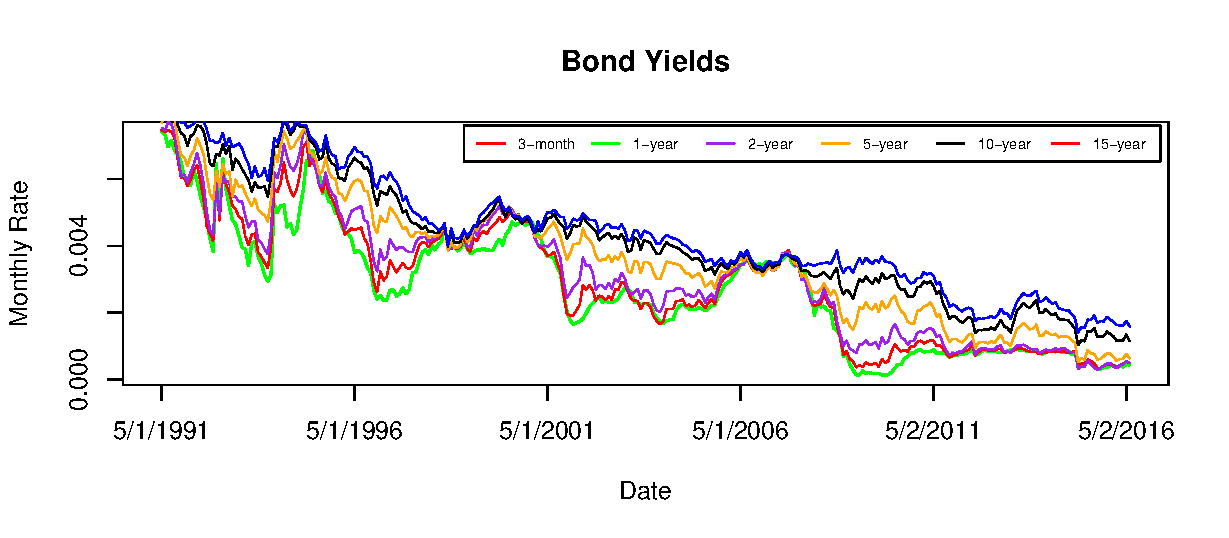
\includegraphics[width=12cm, height=5.3cm]{bondyield.pdf}
			\end{subfigure}
			\begin{subfigure}[t]{0.8\textwidth}
				\centering
				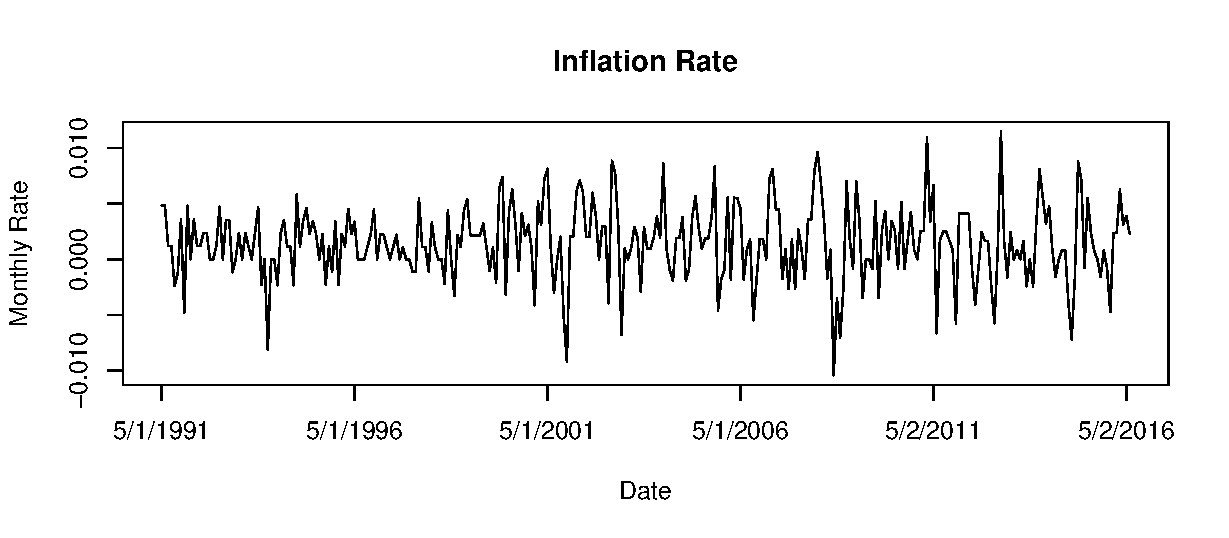
\includegraphics[width=12cm, height=5.3cm]{inf.pdf}
			\end{subfigure}
			\begin{subfigure}[t]{0.8\textwidth}
				\centering
				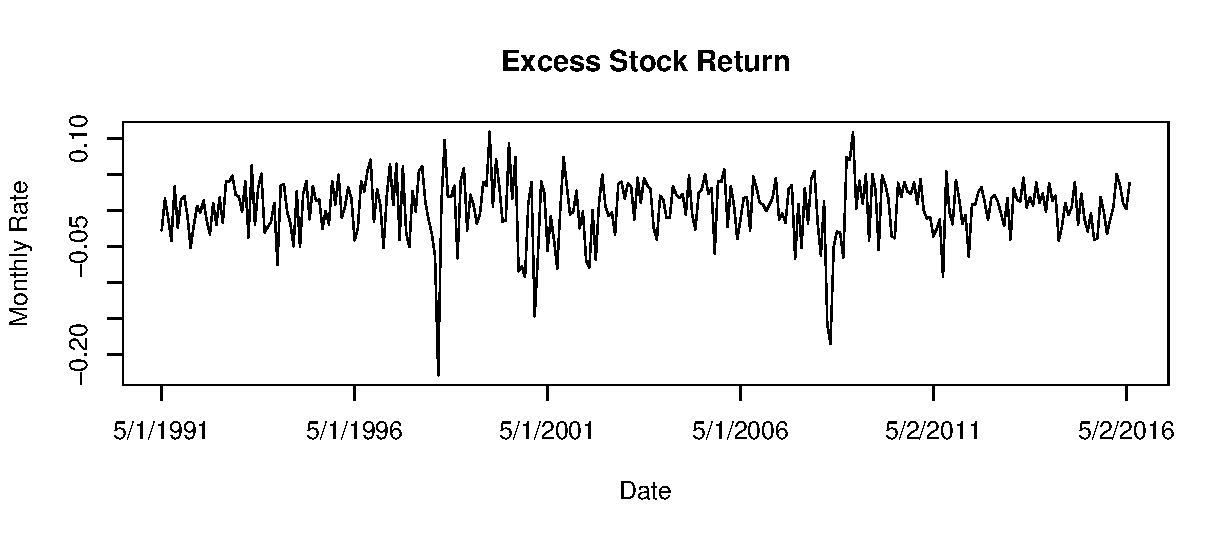
\includegraphics[width=12cm, height=5.3cm]{exc.pdf}
			\end{subfigure}
			\begin{subfigure}[t]{0.8\textwidth}
				\centering
				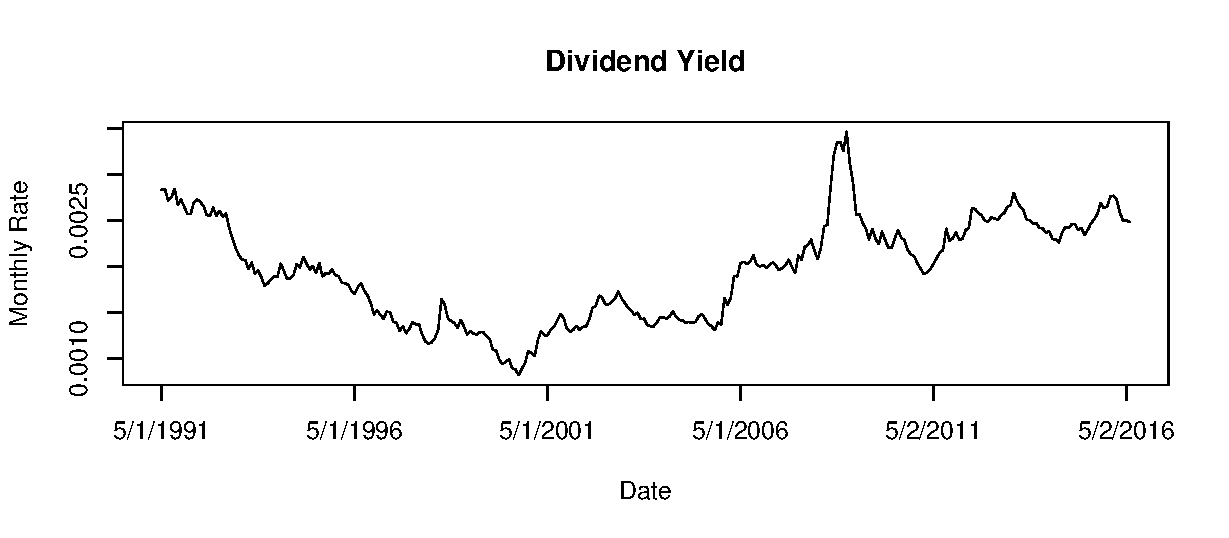
\includegraphics[width=12cm, height=5.3cm]{div.pdf}
			\end{subfigure}
			\caption[Historical Data Plot]{\textbf{Historical Data Plot} \newline\footnotesize \justify The figures show the historical data of the economic variables. The yields and returns are all converted to continuously compounded monthly rate.}
			\label{fig:Historical Data Plot}
		\end{figure}
		
	
	
	\section{Estimation Results}
	\label{Estimation Results}
	
		\justify
		Panel (a) of Table \ref{table:Parameter Estimate of the VAR-GARCH Model} shows the estimated parameters, with $p$-values coming from $Z$-tests included in parentheses, for the VAR-GARCH model. The $p$-values are for testing whether the estimated parameters are significantly different from $0$. From the VAR estimate, we can observe that both the log transform of the short-term and the long-term bond yields are well explained by their own lagged value and the inflation rate. The $R^2$ values in the last column of the table, which is calculated as the variation explained by the model divided by the total variation of the data, measure how much the model explains the variation in the data. We can observe that the model explains a large proportion of the variations in the short-term and long-term bond yields with $R^2$ values as high as $98.13\%$ and $98.79\%$, respectively. Inflation rates appear to be weakly related to lagged values, with an $R^2$ of $4.72\%$. On the other hand, historical excess stock returns are consistent under our model with a white noise process, in which the current value and the lagged value have little relationship and have no significant autocorrelations with other economic variables. The $R^2$ of this variable is $1.05\%$. The relationship between the excess stock return and the dividend yields is significant. Dividend yields rise if stock prices decline and a higher dividend yield predicts an increase in the excess stock returns for the next period. The variability in the dividend yields is also well explained by the model with the $R^2$ equal to $99.44\%$.  The absolute values of the eigenvalues of the $\beta$ matrix are $0.9933$, $0.9783$, $0.9783$, $0.1294$ and $0.0489$. Since they are all smaller than $1$, the stationarity condition of the VAR process is satisfied.
		\begin{table}[!ht]\footnotesize
			\centering
			\resizebox{\linewidth}{!}{
				\begin{tabular}{ccccccc}
					\toprule
					\textbf{(a) VAR Estimate} ($\boldsymbol{\beta}$) & $\ln(r^{s}_t)$     & $\ln(r^{l}_t)$  & $i_t$        & $r_t$       & $\ln(d_t)$ &$R^2$\\
					\midrule
					$\ln(r^{s}_{t+1})$   &0.97274   &0.05668   &-0.61300  &-0.29114  &-0.03143    &0.98138\\
					&(0.00000) &(0.01104) &(0.72027) &(0.00852) &(0.00048)\\
					$\ln(r^{l}_{t+1})$   &0.00151   &0.98779   &0.14012   &-0.11352  &0.00138     &0.98797 \\
					&(0.75795) &(0.00000) &(0.86633) &(0.03118) &(0.80196)\\
					$i_{t+1}$           &-0.00002  &-0.00011  &0.13351   &0.00239   &-0.00129    &0.04721\\
					&(0.95951) &(0.85406) &(0.00523) &(0.45318) &(0.00022)\\
					$r_{t+1}$           &-0.00239  &0.00324   &-0.41396  &0.03639   &0.00754     &0.01058\\
					&(0.61996) &(0.69250) &(0.50446) &(0.48594) &(0.03745)\\
					$\ln(d_{t+1})$       &0.00045   &-0.00844  &-0.07619  &-1.06080  &0.99801     &0.99446\\
					&(0.58370) &(0.00000) &(0.59563) &(0.00000) &(0.00000)\\
					
					\midrule
					& $\ln(r^{s}_t)$     & $\ln(r^{l}_t)$  & $i_t$        & $r_t$       & $\ln(d_t)$\\
					\midrule
					$\boldsymbol{\nu}$ &-0.05370  &-0.04947  &-0.00751 &0.05101  &-0.05611 \\
					
					$\boldsymbol{\gamma}$ &-0.50000  &-0.50000  &0      &0.20391    &-0.5000 \\
					
					\toprule
					
					
					\textbf{(b) GARCH Estimate}   & $\ln(r^{s}_t)$     & $\ln(r^{l}_t)$  & $i_t$        & $r_t$       & $\ln(d_t)$\\
					\midrule
					$\omega_i$  &0.00057   &0.00029   &0.00000   &0.00006   &0.00011\\
					&(0.35186) &(0.29881) &(0.79165) &(0.77700) &(0.00000)\\
					$a_i$       &0.26859   &0.16820   &0.05688   &0.10179   &0.82056\\
					&(0.00028) &(0.00074) &(0.00006) &(0.0100)  &(0.00000)\\
					$b_i$       &0.72141   &0.72434  &0.93082    &0.86577   &0.16944\\
					&(0.00000) &(0.00001) &(0.00000) &(0.00000) &(0.00000)\\
					\midrule
					\textbf{Unconditional}\\
					\textbf{Variance}    &0.05700  &0.00274  &0.00001 &0.00185  &0.01131\\
					
					\bottomrule
				\end{tabular}
			}
			\caption[Parameter Estimate of the VAR-GARCH Model]{\textbf{Parameter Estimate of the VAR-GARCH Model}
				\vspace{-0.4cm}
				\newline\footnotesize\justify The VAR-GARCH parameters are estimated using the maximum likelihood method. Panel (a) shows the estimates of the mean process, including the autoregressive matrix ($\boldsymbol{\beta}$), the constant vector ($\boldsymbol{\nu}$) and the convexity correction and equity risk premium vector ($\boldsymbol{\gamma}$). Panel (b) shows the estimates of the GARCH parameters. The last row of the table shows the unconditional variance levels of the five economic variables calculated from the GARCH estimates.}
			\label{table:Parameter Estimate of the VAR-GARCH Model}
		\end{table}
	
	
		\justify
		Panel (b) of Table \ref{table:Parameter Estimate of the VAR-GARCH Model} shows the estimates of the GARCH parameters and the estimated unconditional variance levels for the five economic variables. In the GARCH model, relatively high $a_i$ and low $b_i$ indicate a more volatile variance than those with relatively low $a_i$ and relatively high $b_i$. From the GARCH parameter estimates, we can see that the dividend yield has the most volatile variances when compared to the other variables, while the inflation process has the most stable variance. This can be confirmed by looking at the historical residual plots of Figure \ref{fig:Residuals Plot}, where we can see that the change in the variations of short rate and dividend yield is much higher than the other variables. The GARCH process is stationary since the sum of $a_i$ and $b_i$ is smaller than $1$ for each variable.
		
		\begin{figure}[h]
			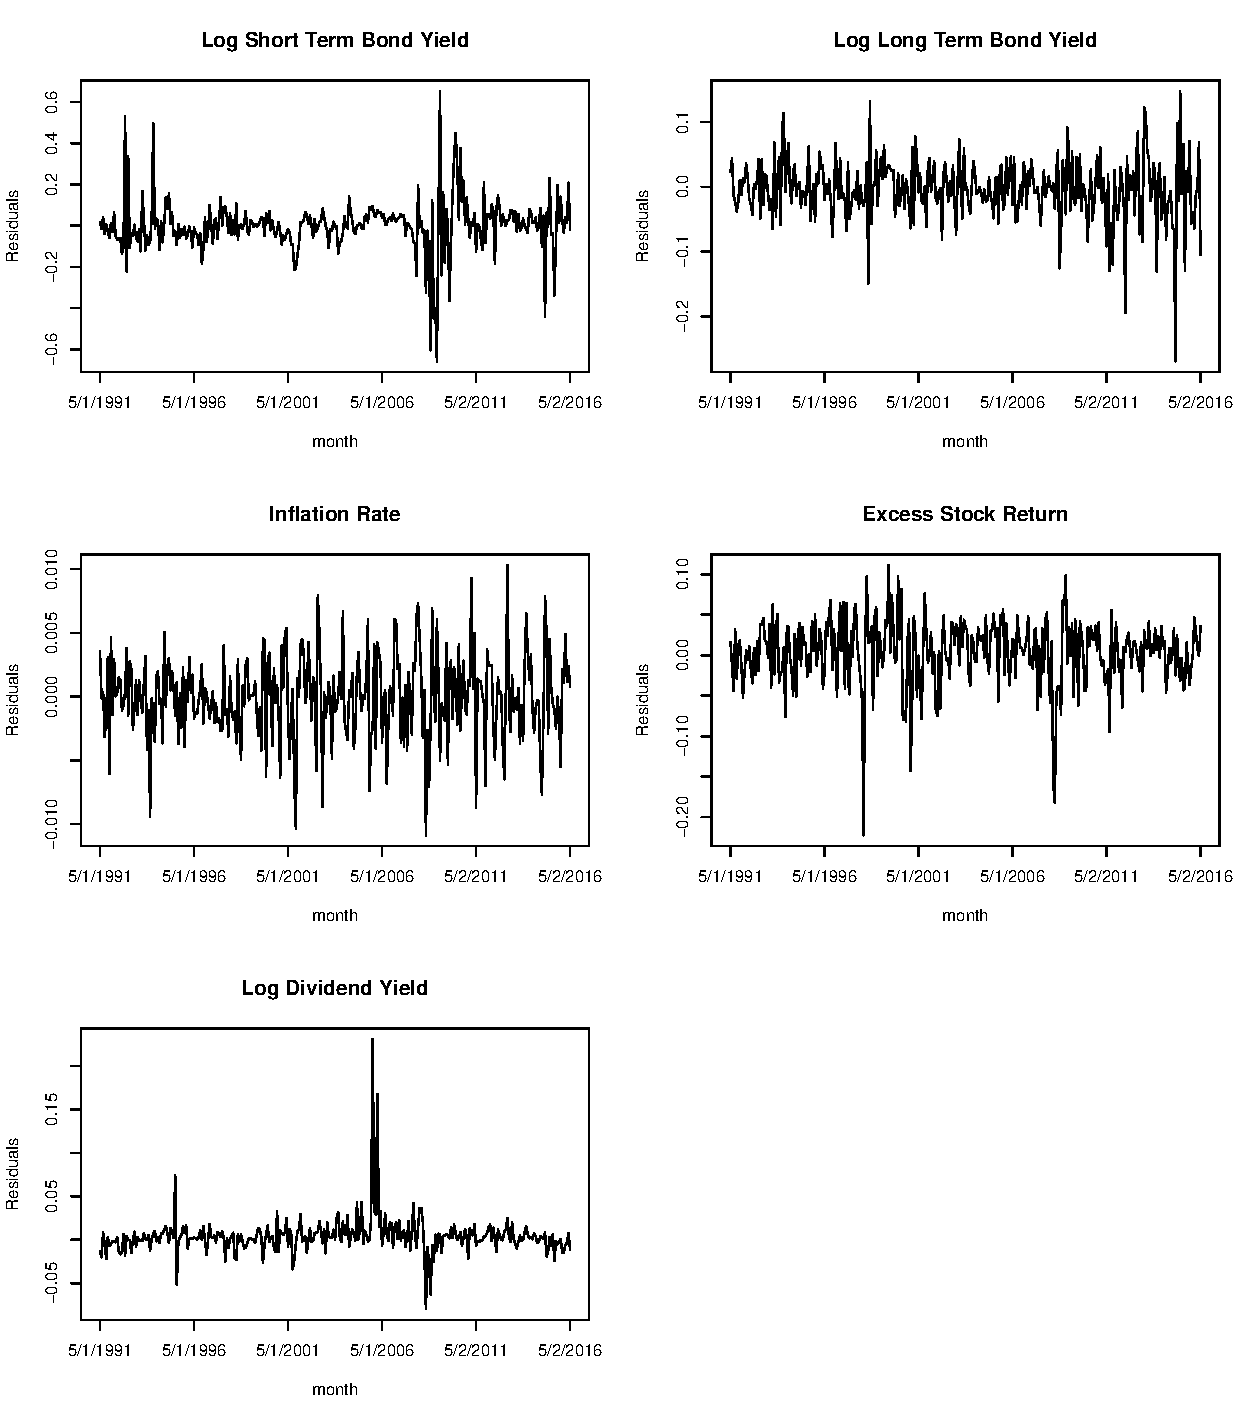
\includegraphics[width=1\linewidth]{HistRest.pdf} 
			\caption[Residuals Plot]{\textbf{Residuals Plot}
				\vspace{-0.4cm}
				\newline\footnotesize \justify The figures show the VAR-GARCH residuals for the five economic variables. The residual values are calculated by subtracting the mean predicted value of the VAR-GARCH model from historical data.}
			\label{fig:Residuals Plot}
		\end{figure}
		
	
		\justify
		The unconditional variances levels for the economic variables are calculated from the GARCH parameters. The unconditional variance levels for the short-term yield is higher than the corresponding variance of the long-term yields. Since we are modelling the logarithmic transform of the bond yields and dividend yields, the unconditional variances levels of these variables are not on the same scale as the inflation rates and excess stock returns and they are therefore not readily comparable. 
	
	
		\justify
		The estimates for the risk premium parameters are given in Table \ref{table:Parameter Estimate of the Risk-Neutral Model}. With these estimates, the value of our objective function in Equation \eqref{eq:EMR_12} is 0.0133. Figure \ref{fig:Historical fit of term structure model} shows the historical fit of the term structure graphically. The dashed lines represent the fitted series and the solid lines represent the actual series. The bond yields produced by the model are very close to the actual bond yields, especially for longer term bonds.  
		\begin{figure}[h]
			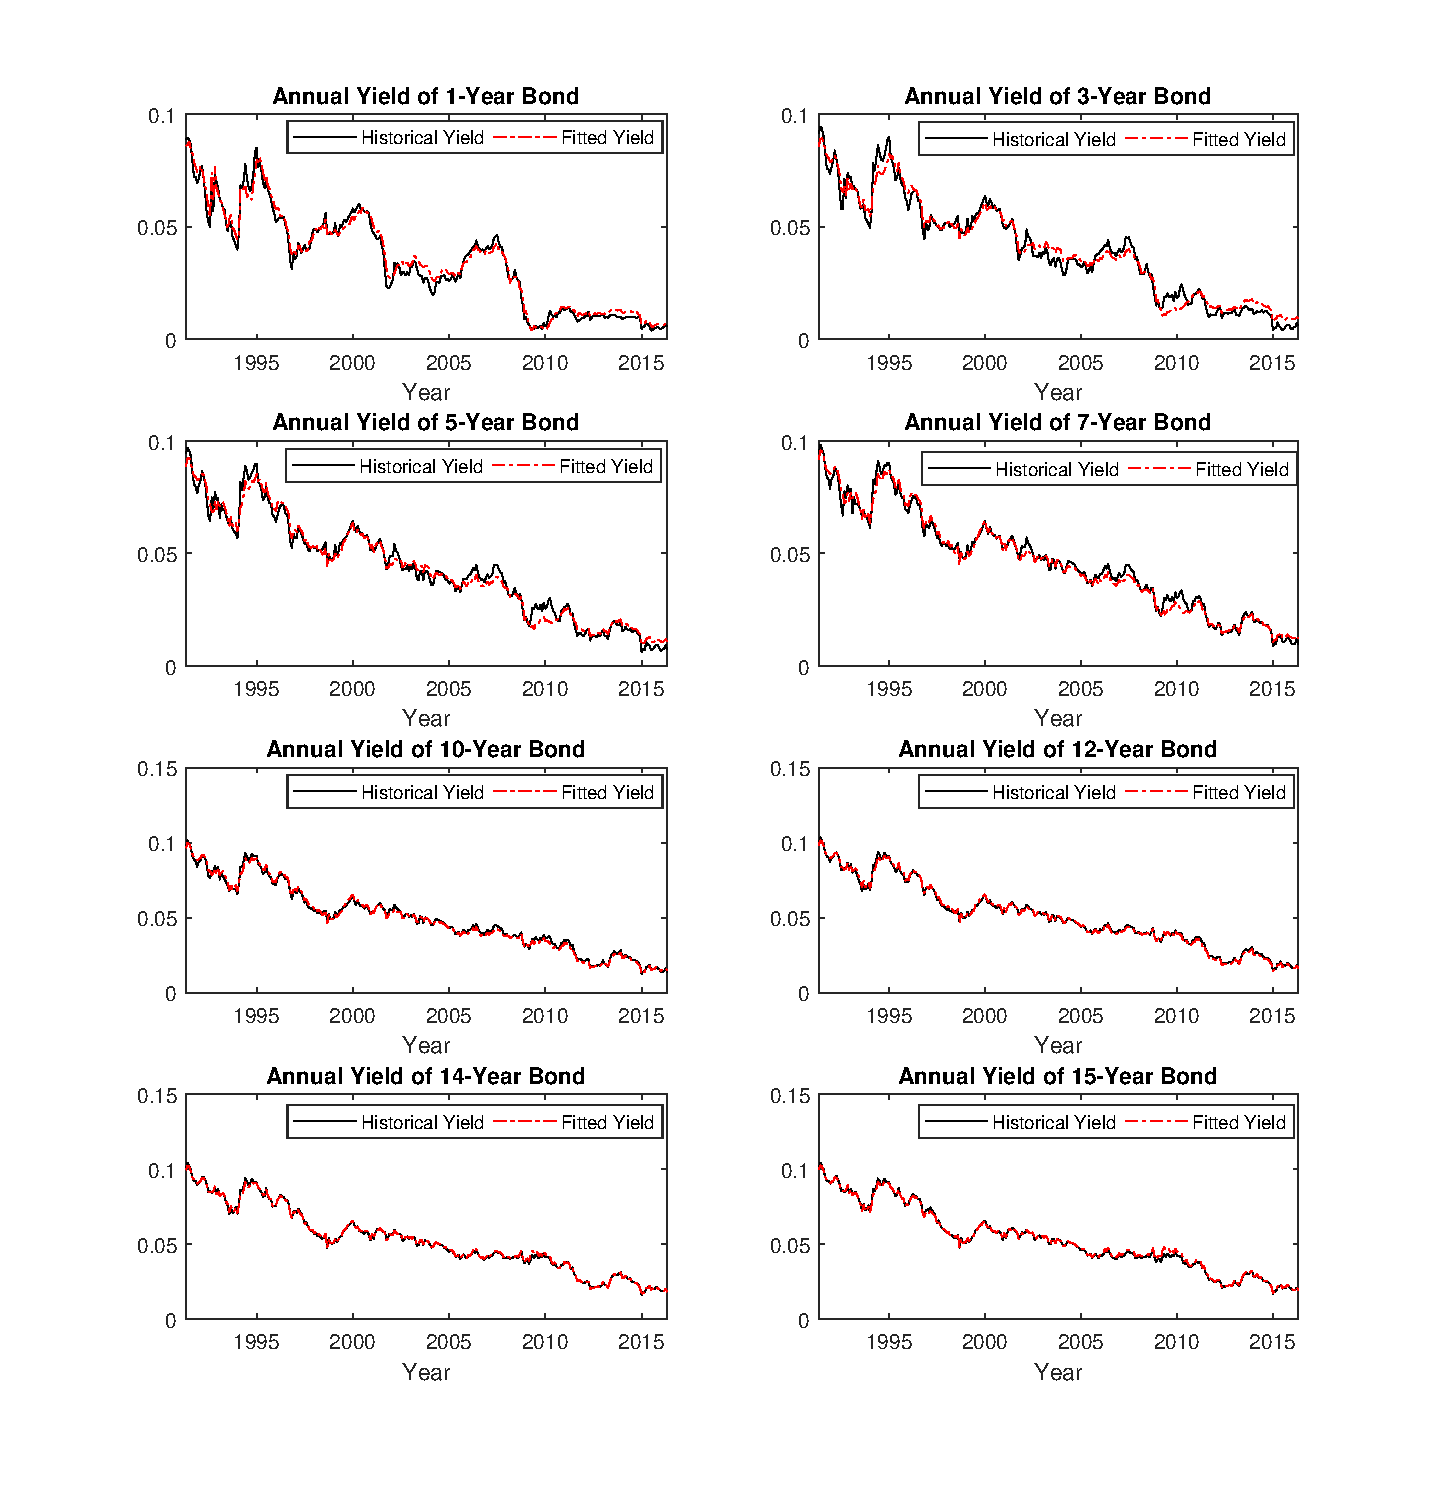
\includegraphics[width=1.1\linewidth]{ResultPlot/rnfit.pdf} 
			\caption[Historical Fit of Term Structure Model]{\textbf{Historical Fit of Term Structure Model}
				\vspace{-0.4cm}
				\newline\footnotesize \justify The figures show the historical fit of the risk-neutral model for zero-coupon bond yields for bonds with eight different maturities. The red line represents the model yields and the black line represents the historical yields.}
			\label{fig:Historical fit of term structure model}
		\end{figure}
	
	
		\justify
		\begin{table}[!ht]\footnotesize
			\centering
			\resizebox{\linewidth}{!}{
				\begin{tabular}{ccccccc}
					\toprule
					\textbf{Risk Premium Parameters} &$\boldsymbol{\lambda_0}$ & &  &$\boldsymbol{\lambda_{1}}$  & &\\
					\cmidrule(r){3-7}
					& & $\ln(r^{s}_t)$     & $\ln(r^{l}_t)$  & $i_t$        & $r_t$       & $\ln(d_t)$     \\
					\midrule
					$\ln(r^{s}_t)$   &-0.0010 &0.0436 &-0.0291  &3.3698 &-0.0475  &-0.0110 \\
					$\ln(r^{l}_t)$   &-0.0612 &0.0047  &-0.0142 &-0.3890  &-0.1024 &-0.0012 \\
					$i_t$            &0 &0 &0 &0  &0  &0  \\
					$r_t$            &0.0510  &-0.00239 &0.00324 &-0.41396 &0.03639  &0.00754\\
					$\ln(d_t)$       &0 &0 &0 &0  &0  &0  \\    
					\bottomrule
				\end{tabular}
			}
			\caption[Parameter Estimate of the Risk-Neutral Model]{\textbf{Parameter Estimate of the Risk-Neutral Model}
			\newline\footnotesize \justify The risk premium parameters $\boldsymbol{\lambda_{0}}$ and $\boldsymbol{\lambda_{1}}$ are calibrated by minimizing the total squared differences between the model zero-coupon bond yields and the actual zero-coupon bond yields.}
			\label{table:Parameter Estimate of the Risk-Neutral Model}
		\end{table}
	
		\justify
		Table \ref{table:Statistics of the Historical Mispricing Term Structure} shows the mispricing of the fitted bond yield term structure. From the table, we can also observe that the fit is worse on the short end of the yield curve. On average, our model overpriced the $1$-year bond yield by $0.89\%$, which is the highest mispricing shown in the table.  


		\begin{table}[!ht]
			\centering
			\resizebox{\linewidth}{!}{
				\begin{tabular}{cc c c c c c c c}
					\toprule
					& $r^{(12)}$  &$r^{(36)}$  &$r^{(84)}$  &$r^{(120)}$  &$r^{(144)}$   &$r^{(168)}$  \\
					\midrule
					Mean               & 0.00089 &0.00038   &-0.00045   &-0.00034   &-0.00011    &0.00015    \\
					Standard Deviation &0.00288    &0.00373     &0.00256    &0.00153    &0.00097      &0.00075\\
					\bottomrule
				\end{tabular}
			}
			\caption[Statistics of the Historical Mispricing Term Structure]{\textbf{Statistics of the Historical Mispricing Term Structure}
			\newline\footnotesize \justify The difference between the model bond yield and the actual bond yield is calculated for the $302$ historical time points. The first row of the table shows the averages of the differences for bonds with different maturities and the second row shows the standard deviation of these differences.}
			\label{table:Statistics of the Historical Mispricing Term Structure}
		\end{table}
	
	
	\section{Forecasts}
	\label{Forecasts}

		\justify
		We generate $10,000$ scenarios each under $\mathbb{P}$- and $\mathbb{Q}$-measures. The real-world scenarios are generated for the purpose of simulating the actual operation of the pension fund, while the risk-neutral scenarios are used to price the embedded options in the pension contract. The first step of the forecasting is choosing the starting value of the simulation. It can be selected in different ways depending on the focus of the research. In this project, we start our simulation at the long-term equilibrium levels of the five economic variables, so that the value transfers in the pension plan are due only to the plan provisions and not to any particular patterns in the financial market. The equilibrium levels of the economic variables expressed in continuously compounded annual rates are displayed in Table \ref{table:Equilibrium Levels of Economic Variables}.

		\justify
		\begin{table}[!ht]
			\centering
			
			\begin{tabular}{ccccc}
				\toprule
				Short-Term  & Long-Term  &Inflation  &Excess Stock  &Dividend \\
				Bond Yield  & Bond Yield & Rate      &Return        & Yield\\
				\midrule
				$0.0210$   &$0.0408$    &$0.0208$    &$0.0120$     &$0.0220$ \\
				\bottomrule
			\end{tabular}
			
			\caption[Equilibrium Levels of Economic Variables]{\textbf{Equilibrium Levels of Economic Variables}
			\newline\footnotesize \justify This table shows the future long-term equilibrium level of the five economic variables in our model.}
			\label{table:Equilibrium Levels of Economic Variables}
		\end{table}


		\vspace{-0.4cm}
		\justify
		After the starting values are determined, we generate the future real-world scenarios by forwardly iterating the VAR-GARCH model defined in Equations \eqref{eq:ESG_3} and \eqref{eq:ESG_5}. The future scenarios under the $\mathbb{Q}$-measure are generated in the same way with the risk-neutral model defined in Equations \eqref{eq:ESG_19} to \eqref{eq:ESG_21}. The innovation terms are drawn stochastically from a multivariate normal distribution with a mean of zero and the appropriate GARCH variance-covariance matrix. Economic scenarios are generated in monthly steps for a time horizon of $55$ years. The simulation horizon is determined such that the youngest participants in the pension plan at the start of the study can receive their last retirement benefit by the end of the simulation. The funnel of doubt for the real-world dynamics of the five variables in the next $55$ years are shown in Figure \ref{fig:Funnel of Doubt for Evolution of Simulated Economic Variables}.
    		\begin{figure}[h]
			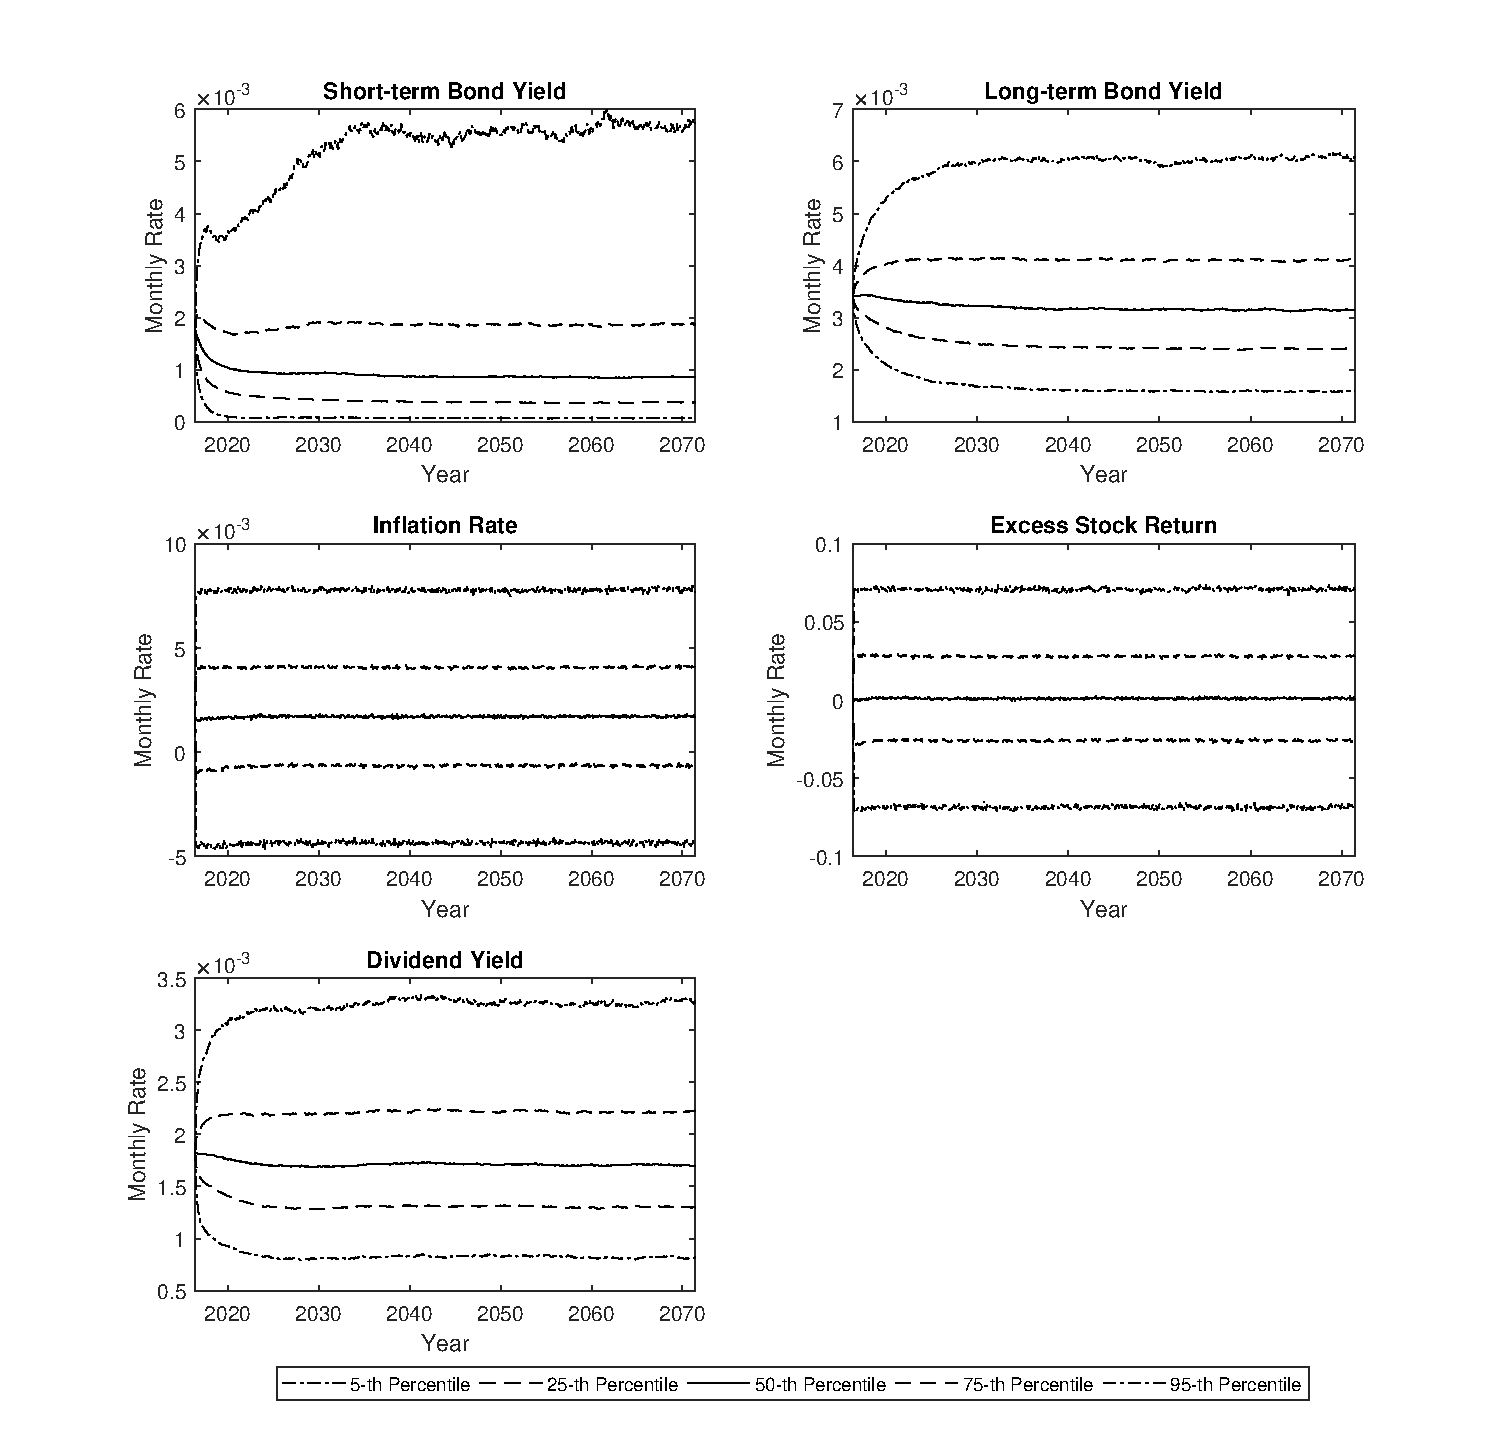
\includegraphics[width=1\linewidth]{ResultPlot/projrate.pdf} 
			\caption[Funnel of Doubt for Evolution of Simulated Economic Variables]{\textbf{Funnel of Doubt for Evolution of Simulated Economic Variables}
				\vspace{-0.4cm}
				\newline\footnotesize \justify Future evolution of the five economic variables are projected using Monte Carlo simulation. We generate $10{,}000$ paths for each economic variable. The figures show the $5^{\text{th}}$, $25^{\text{th}}$, $50^{\text{th}}$, $75^{\text{th}}$, and $95^{\text{th}}$ percentiles of the simulated distribution of the five economic variables.}
			\label{fig:Funnel of Doubt for Evolution of Simulated Economic Variables}
		\end{figure}    
        

		\justify
		In this research, the pension plans are assumed to have an annual valuation frequency, therefore all the monthly simulated rates are converted into annual effective rates for later use. The annual effective inflation rate $\tilde{i_{t}}$ in year $t$ can be obtained directly from the simulations:
		
		\begin{equation}
		\label{eq:EMR_18}
		%\tilde{i_{t}} = \exp\bigg(\sum_{j=12(t-1)+1}^{12t}i_{j}\bigg) - 1 .
		\tilde{i_{t}} = \exp\left(\sum_{j=12(t-1)+1}^{12t}i_{j}\right) - 1 .
		\end{equation}
	
	
		\justify
		Since we are modelling the logarithmic transform of the bond yields and dividend yields, they are first transformed back by taking the exponential of the values in the simulated time series. Then, these yields can be converted to effective annual rates by applying the following transformations:
		\begin{align}
		\tilde{r}_{t}^s = &\,\exp(12\,r_{12(t-1)+1}^s)-1,\\
		\tilde{r}_{t}^l = &\,\exp(12\,r_{12(t-1)+1}^l)-1,\\
		\tilde{d}_{t} = &\,\exp\bigg(\sum_{j=12(t-1)+1}^{12t}d_{j}\bigg) - 1.
		\end{align}
		
		\justify
		The continuously compounded monthly stock return $sr_{j}$ for month $j$ can be obtained by adding the short-term bond yield $r_{j}^s$ and the excess stock return $s_{j}$:
		\begin{equation}
		\label{eq:EMR_19}
		sr_{j} =  r_{j}^s + s_{j},
		\end{equation}
		where $j=1,...,660$. Then, the effective annual stock return $\widetilde{sr}_{t}$ in year $t$ is calculated as
		\begin{equation}
		\label{eq:EMR_20}
		\widetilde{sr}_{t} = \exp\bigg(\sum_{j=12(t-1)+1}^{12t}sr_{j}\bigg) - 1. 
		\end{equation}
	
	
	
	\chapter{Stylized Target Benefit Plan: Key Features and Assumptions}
	\label{Stylized Target Benefit Plan: Key Feature and Assumption}
	
		\justify
		In this chapter, we introduce the liability model for our stylized pension fund, including the membership profile, the salary increase experience, and the key assumptions for recognizing accrued liabilities before plan inception. The TBP design elements are discussed in detail, consisting of the target benefit, the contribution rate and the decision making process regarding the benefit adjustments. 
	
	
	\section{Plan Membership Assumptions}
	\label{Plan Membership Assumptions}
		
		\justify
		We assume a stationary plan membership with the following characteristics:
		
		\begin{itemize}
			\item All members enter the plan at age $e=30$ and retire at age $r=65$;
			\item All members die at age $\omega = 86$;
			\item There are no decrements before age 86.
			\item There are $100$ new members of age 30 that enter the plan each year;
			\item The number of members aged $x$ in the plan is represented by $n_{x} = 100$ for $30<x<86$, and $0$ otherwise;
		\end{itemize}
		
		\justify
		This membership profile is chosen for the sake of simplicity. We do not consider randomness in mortality as the assumed age at death is the same for all members. Specifically, the age at death, $\omega$, is selected such that the annuity value is equal to the present value of a whole-life annuity, i.e.,
		\begin{equation}
		\label{eq:STBP_1}
		\ddot{a}_{\angl{\omega-65}} = \ddot{a}_{65},
		\end{equation}
		
		\justify
		where $\ddot{a}_{65}$ is calculated according to the 2014 Canadian Pensioners Mortality Table for males. The membership of the plan is mature and stationary since the inception of the plan, and because all members are assumed to die exactly at age $86$, the plan has $56$ cohorts of equal size at any given point in time.
	
	
	\section{Salary Progression}
	\label{Salary Progression}
	
		\justify
		Salaries increase at the beginning of each year at the same rate for all generations. The growth rate in any given year $t$ consists of two components:
		\begin{itemize}
			\item The inflation rate in year $t$ as defined in Section \ref{Forecasts}, $\tilde{i_t}$;
			\item The annual rate of salary increase for promotion and merit $m$, which is equal to $0.5\%$.
		\end{itemize}
		The total salary increase in year $t$ for all active members can be calculated as
		\begin{equation}
		\label{eq:STBP_2}
		s_{t} = (1+\tilde{i}_t)(1+m)-1.
		\end{equation}
		We assume that the starting salary of the new entrants at time 0 is $\$50,000$. Let $S_{x,t}$ denote the salary of a member aged $x$ at time $t$. Therefore, the relationship between the salary of different cohorts at different times can be expressed by the following equations:
		\begin{align}
		S_{x+1,t} = &\, S_{x,t}\,(1+m), \label{eq:STBP_3}\\
		S_{x,t+1} = &\, S_{x,t}\,(1+\tilde{i}_t), \label{eq:STBP_4}\\
		S_{x+1,t+1}=&\, S_{x,t}\,(1+m)(1+\tilde{i}_t) = S_{x,t}\,(1+s_{t}). \label{eq:STBP_5}
		\end{align}

	
	\section{Contribution Rate}
	\label{Contribution Rate}
	
		\justify
		The contribution rate $c$ is fixed and is equal to $10.6\%$ of payroll for all generations. The annual contribution is paid at the beginning of each year. Let $C_{x,t}$ denote the contribution paid at time $t$ in respect of an active member aged $x$, expressed as
		\begin{equation}
		\label{eq:STBP_6}
		C_{x,t} = c \, S_{x,t}.
		\end{equation}
		The total contributions made to the plan at time $t$ are
		\begin{equation}
		\label{eq:STBP_7}
		C_{t} = \sum_{x=30}^{64} n_x \, C_{x,t}.
		\end{equation}
	
	
	\section{Target Benefit}
	\label{Target Benefit}
	
		\justify
		The target benefit at time $t$ for a member age $x$ is expressed as a percentage $b_{x,t}$ of the projected final year earnings multiplied by the number of years of service. The percentage $b_{x,t}$ is the target annual accrual rate applicable to all service (i.e., past and future). It can be separated into two components: 
		\begin{itemize}
			\item $b_{x,t}^p$, which is the target accrual rate applicable to past service (that is, service up to time $t$);
			\item $b_{x,t}^f$, which is the target accrual rate applicable to future service (that is, service after time $t$).
		\end{itemize}
		
		\justify
		In practice, either or both of these two components might be adjusted at each valuation based on the result of the affordability test, and the pre-defined triggers and actions. In this research, the initial target annual accrual rate is set at $1\%$ for all cohorts, i.e., $b_{x,0}^p = b_0 = 1\%, \text{ for all } x$.
		
		
		\justify
		For active members, the amount of the target benefit at each valuation date is implicitly indexed with inflation because the inflation experience is reflected in the projected final year earnings. The retirement benefits are paid out at the beginning of each year according to the amount of the then-current target benefit for past service. The target benefit $TB_{x,t}$ at time $t$ of an active member aged $x$ is
		\begin{equation}
		\label{eq:STBP_8}
		TB_{x,t} =  \left[ b_{x,t}^p\, (x-30) + b_{x,t}^f \,(65-x)\right] \, PFS_{x,t}, \quad x<64,
		\end{equation}
		where $PFS_{x,t}$ is the salary that a member aged $x$ at time $t$ is projected to earn in his final year of employment (i.e., just before retirement). The salary is projected under the assumption of a constant future inflation rate $\tilde{i}^{f} = 2\%$, thus,
		\begin{equation}
		\label{eq:STBP_9}
		PFS_{x,t} = S_{x,t}\,\left[(1+m) (1+\tilde{i}^f)\right]^{64-x}.
		\end{equation}
		For a retired member, the target benefit is calculated using the actual final year's earnings: 
		\begin{equation}
		\label{eq:STBP_10}
		TB_{x,t} = b_{x,t}^{p} \,(65-30) \, S_{64,t-(x-64)},\quad x\geqslant 65.
		\end{equation}
		The annual pension entitlement $B_{x,t}$ for a retiree aged $x$ at time $t$ is equal to $TB_{x,t}$, and the total benefits paid from the plan at time $t$ are:
		\begin{equation}
		\label{eq:STBP_11}
		B_{t} = \sum_{x= 65}^{85} n_x \, B_{x,t}.
		\end{equation}


	
	\section{Starting Asset Value}
	\label{Starting Asset Value}


		\justify
		We assume that all members who are older than age 30 have their own DC funds before joining the target benefit plan, and that the new plan starts with all members bringing all their individual funds into the group fund. The account value of the individual DC fund for a member aged $x$ at plan inception ($AVDC_{x,0}$) is determined on the basis of the following assumptions:
		
		\begin{itemize}
			\item Past contributions were made at the rate of $10.6\%$ of the annual salary per year since entry to the DC plan at age $30$.
			
			\item Past salary increases consisted of the same $m$ and a constant historical inflation rate $\tilde{i}^h$ of $2\%$ per year. The past salary $S_{x-t,-t}$ at time $-t$ of a member who is aged $x$ at plan inception is calculated backward from the time $0$ salary:
			\begin{equation}
			\label{eq:STBP_12}
			S_{x-t,-t} = S_{x,0}\left[(1+m)(1+\tilde{i}^h)\right]^{-t},
			\end{equation}
			for $t\leqslant x - 30$. Note that $S_{x-t,-t}$ is nil for years before the member turns $30$ (i.e., $t>x-30$).
			
			\item The DC fund was invested in a rolling portfolio of zero-coupon bonds with 15-year maturity, and we assume that the historical annual return $\tilde{r}^{h} = 4.1\%$ of this portfolio was constant over time, which is the corresponding long-term bond yield at time $0$. More details on the selection of this rate are given in Section \ref{Affordability Test}.
			
			\item For a member who retired before plan inception, the account value is reduced by the benefit payment made from the individual DC fund. The retirement benefit $B^{h}_{x-t,-t}$ paid out at time $-t$ to a member aged $x$ at time $0$, is assumed to be:
			\begin{equation}
			\label{eq:STBP_13}
			B^{h}_{x-t,-t} = 0.01\, (65-30) \, S_{64,x-65}.
			\end{equation}
		\end{itemize}
	
		\justify
		The third and fourth assumptions are made for internal consistency with the affordability test outlined in the next section. Under these assumptions, the account value $AVDC_{x,0}$ of a member age $x$ at plan inception can be calculated as
		\begin{equation}
		\label{eq:STBP_14}
		AVDC_{x,0} = 
		\left\{
		\begin{array}{ll}
		\sum\limits_{t=1}^{x-30}c\,S_{x-t,-t}\,(1+\tilde{r}^{h})^t &\text{ if } x\leqslant 65\\
		\sum\limits_{t=x-64}^{x-30}c\,S_{x-t,-t}\,(1+\tilde{r}^{h})^t - \sum\limits_{t=1}^{x-65} B^{h}_{x-t,-t}(1+\tilde{r}^{h})^t &\text{ if } x>65\\
		\end{array}
		\right..
		\end{equation}


	
		\justify
		The starting asset value, $F_{0}$, of the TBP is the total value of the individual DC funds of all plan members at $t=0$:
		\begin{equation}
		\label{eq:STBP_15}
		F_{0} = \sum_{x=30}^{85} n_{x}\, AVDC_{x,0} = 748,870,000.
		\end{equation}
		Although the contributions can be adjusted within a limited range under certain plan designs, we choose to have a fixed contribution rate as well as the same starting asset to make sure that the plan costs are consistent across various designs.
	
	
	\section{Affordability Test}
	\label{Affordability Test}
	
		\justify
		The affordability test is performed at each valuation date to decide whether the target accrual rate determined previously is still affordable. In this research, the valuation time is the beginning of each year, before any contributions and benefit payments. Given the availability of funds and the future contribution commitment, there are two crucial elements that will affect the result of the affordability test: the valuation assumptions and the valuation methods used to evaluate the plan assets and liabilities.
	
	
	
	\subsection{Valuation of Plan Assets}
	\label{Valuation of Plan Assets}
	
		\justify
		For the plan assets, we assume that all the available funds are invested in equities and fixed-income assets. The actuarial value of the plan assets is taken as the market value of all the invested assets. We use the TSX/S\&P Composite index to model equity returns and the future evolution of the annual effective returns is obtained directly from the simulation results of the VAR-GARCH model in Equation \eqref{eq:EMR_15}. For the fixed income allocation, we assume the fund owns 15-year zero-coupon bonds only. The maturity of the bond portfolio is reset every year by selling all remaining bonds with 14 year maturity and purchasing new 15-year bonds at the prevailing market price. The annual effective return of the bond portfolio $\tilde{\pi}_{t}^{B}$ in year $t$ can be calculated as
		\begin{equation}
		\label{eq:STBP_17}
		\tilde{\pi}_{t}^{B} = \frac{\hat{P}^{(180)}_{t}-\hat{P}^{(168)}_{t+1}}{\hat{P}^{(180)}_{t}},
		\end{equation}
		where $\hat{P}^{(T)}_{t}$ is the price of a zero-coupon bond paying one dollar in $T$ months at time $t$. 



		\justify
		The asset mix is an important design element of a TBP and it is determined based on the risk preference of the plan. In some TBP designs, the asset allocation can be adjusted from time to time according to pre-specified rules related to the affordability test. In our stylized plan, the asset mix is static with $50\%$ invested in equities and $50\%$ invested in long-term bonds. The asset portfolio is rebalanced each year. We let $r_{t}^P$ be the annual portfolio return in year $t$, calculated as
		\begin{equation}
		\label{eq:STBP_18}
		r_{t}^P =0.5 \, \widetilde{sr}_t + 0.5 \, \tilde{\pi}_{t}^{B}.
		\end{equation}
	
	
		\justify
		The portfolio returns are calculated at each future time point under each simulated economic scenario. Figure \ref{fig:Funnel of Doubt for the Valuation Rate} shows the percentile plots of the fund return distribution over the next $55$ years. 
		\begin{figure}[h]
			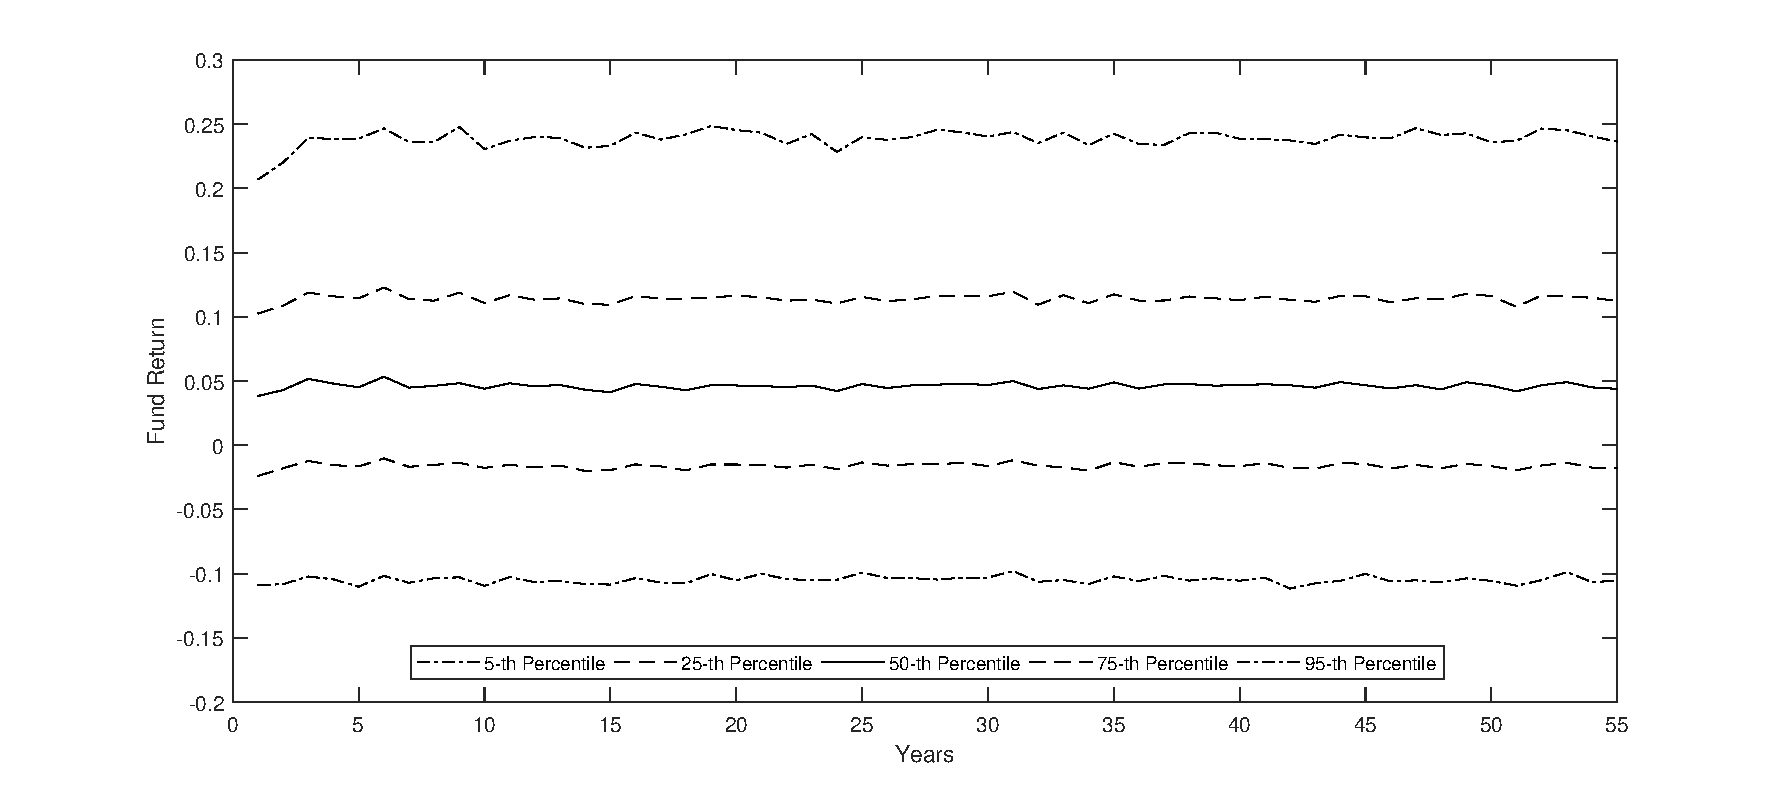
\includegraphics[width=\linewidth]{ResultPlot/frpct1.pdf} 
			\caption[Funnel of Doubt for Evolution of the Fund Returns]{\textbf{Funnel of Doubt for Evolution of the Fund Returns}
				\vspace{-0.4cm}
				\newline\footnotesize \justify The fund return is calculated using Equation (\ref{eq:STBP_18}) under each scenario. The $5^{\text{th}}$, $25^{\text{th}}$, $50^{\text{th}}$, $75^{\text{th}}$, and $95^{\text{th}}$ percentiles of the simulated distribution are shown in the figure.}
			\label{fig:Funnel of Doubt for Evolution of the Fund Returns}
		\end{figure}
	
	
		\justify
		We can observe that the distribution of the fund returns is relatively stable over time. However, the fund returns within any given scenario can be quite volatile. Two sample scenarios of the fund return evolution are shown in Figure \ref{fig:Fund Returns under Two Economic Scenarios}.
		\begin{figure}[h]
			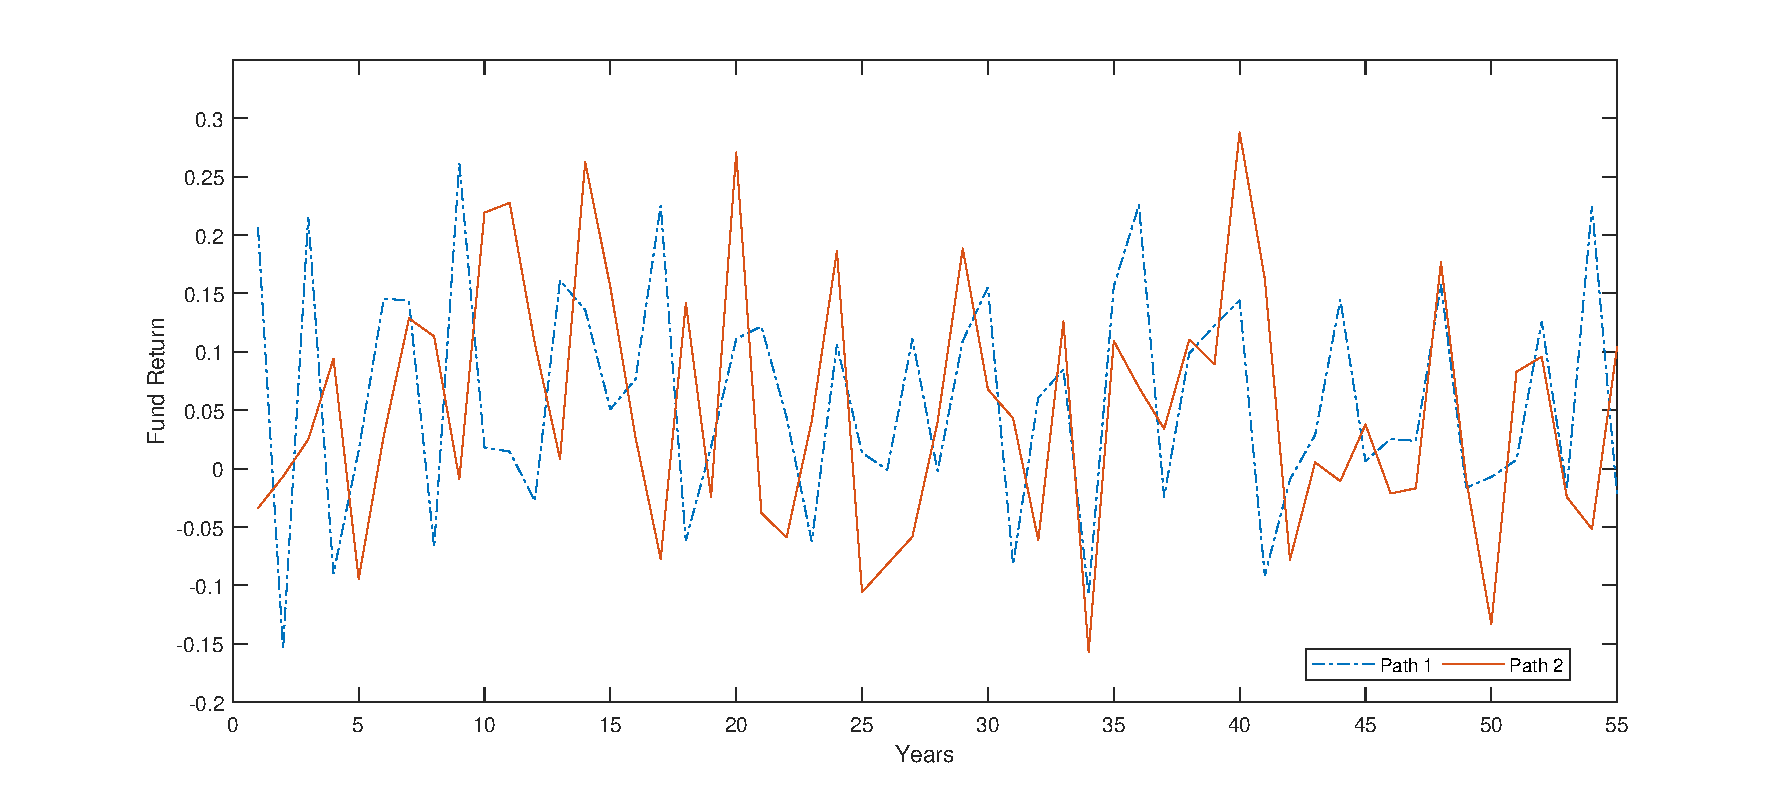
\includegraphics[width=\linewidth]{ResultPlot/fr1scen.pdf} 
			\caption[Fund Returns under Two Economic Scenarios]{\textbf{Fund Returns under Two Economic Scenarios}
				\vspace{-0.4cm}
				\newline\footnotesize \justify This figure shows two paths of the evolution of the future fund returns, which are the first and second scenarios in our simulation.}
			\label{fig:Fund Returns under Two Economic Scenarios}
		\end{figure}
		Based on the returns of the asset portfolio, the actuarial value of the plan assets $F_t$, which is equal to the market value of plan assets, can be expressed recursively as
		\begin{equation}
		\label{eq:STBP_19}
		F_t = (F_{t-1} + C_{t-1} - B_{t-1})\, (1+r_{t}^{P}),
		\end{equation}
		with the starting value $F_{0} = 748,870,000$, given in Equation \eqref{eq:STBP_15}. 
	
	
	\subsection{Valuation of Plan Liability}
	\label{Valuation of Plan Liability}
	
		\justify
		The assumptions needed to value the plan liability relate to mortality, future salary increases and the valuation rate. The mortality assumption used in each valuation is identical to the one in Section \ref{Plan Membership Assumptions}: all members are assumed to die at age 86. The salary increase assumption used in each valuation is a fixed annual rate based on a forward-looking inflation assumption of $2\%$ per year and the $0.5\%$ per year increase for merit and promotion, for a total of $(1.02)(1.005)-1=2.51\%$ per year.
	
		\justify
		The assumed valuation rate can significantly affect how the benefit is adjusted at each valuation date, thus creating different wealth distributions among generations. We compared the following choices for the valuation rate $i_{t}^V$ at time $t$:
		\begin{itemize}
			\item Valuation rate based on long-term bond yields, where $i_{t}^{V}$ is set to the 15-year zero-coupon bond yield $\tilde{r_{t}}^L$;
			\item Valuation rate equal to the expected return on assets, denoted by $EROA_{t}$.
		\end{itemize}
		In this study, the expected return on the assets is constructed by following the ``building block approach'' in the guidance material published by the \citet{cia2015a}. We take the yield on $15$-year zero-coupon bonds at time $t$ as the actuary's best estimate of the long-term returns expected on the bond portion of the pension fund from time $t$ onwards. To estimate long-term returns on the equity portion of the fund we add a fixed risk premium to the 15-year zero-coupon bond yield.\footnote{This approach is frequently used in North America. The same approach is included in the Alberta TBP regulations for calculating the ``benchmark valuation rate'' (\citet{Alberta2014}).} From the historical data, we find that the average risk premium over the 15-year bond yields has been $2.23\%$ for the TSX/S\&P Composite index. Therefore, we set it to $2.23\%$, and the $\text{EROA}_t$ is expressed as
		\begin{equation}
		\label{eq:STBP_20}
		\text{EROA}_t = \tilde{r}_{t}^L + 0.5\, (0.0223).
		\end{equation}
	
	
		\justify
		Note that under both choices of the valuation rate, $i_{t}^V$ is a stochastic rate related to $\tilde{r_{t}}^L$, which varies at each time point under each scenario. Since $\tilde{r_{t}}^L$ may take very small or very large values in some scenarios, we apply a lower bound of $1\%$ and an upper bound of $25\%$ to $i_{t}^{V}$ to prevent unreasonable outcomes. 
	
	
		\justify
		The actuarial value of the plan liabilities also depends on the choice of the valuation method. Popular pension valuation methods include the traditional unit credit method (TUC), the projected unit credit method (PUC), and the entry-age normal method (EAN). In this research, we use the EAN method described in \citet{Aitken1996}. We define: 
		
		\begin{itemize}
			\item $TBF_{x,t}$ as the target benefit in respect of future service for an active member age $x$ at time $t$, before adjustment at time $t$;
			\item $TBP_{x,t}$ as the target benefit in respect of past service for a member age $x$ at time $t$, before adjustment at time $t$; and
			\item $TAL_{t}^{EAN}$ as the total actuarial liability of the plan using the EAN method at time $t$, before adjustment at time $t$.
		\end{itemize}
		Here, ``before adjustment at time $t$'' refers to the fact that the affordability test must be performed using the target accrual rates determined in the previous valuation.\footnote{The adjustment to the target accrual rates at time $t$ can only be made once the result of the affordability test at time $t$ is known.}
	
	
		\justify
		Under the EAN method, the actuarial liability $TAL_{t}^{EAN}$ is equal to the present value of projected benefits less the present value of future normal costs. We split the present value of projected benefits into two components---that corresponding to past service and that corresponding to future service---so that:
		\begin{equation}
		\label{eq:STBP_21}
		TAL_{t}^{EAN} = PVTBP_{t} + PVTBF_{t} -PVFNC_{t}.
		\end{equation}
	
	
		\justify
		First, $PVTBP_{t}$ is the present value of total benefits in respect of past service for all members in the plan at time $t$, prior to making any adjustments to the benefit accrual rate at time $t$,
		\begin{equation}
		\label{eq:STBP_22}
		PVTBP_{t} = \sum_{x=30}^{64}n_{x} \, TBP_{x,t}\, \frac{\ddot{a}_{\angl{86 - 65+1}i^{V}_{t}}}{(1+i^{V}_{t})^{(65-x)}} + \sum_{x=65}^{86}n_{x}\, TBP_{x,t} \, \ddot{a}_{\angl{86 - x }i^{V}_{t}},
		\end{equation}
		where the target benefit in respect of past service, $TBP_{x,t}$, is
		\begin{equation}
		\label{eq:STBP_23}
		TBP_{x,t} = \left\{
		\begin{array}{ll}
		\left[b_{x, t-1}^{p} (x-30-1) + b_{x, t-1}^{f}\right] \, PFS_{x,t} &\text{ if }x<65\\
		b_{x, t-1}^{p}  \, (65-30) \, S_{64,t-(x-64)} &\text{ if }x\geqslant 65\\
		\end{array}
		\right..
		\end{equation}
	
	
		\justify
		This is the target benefit that each member would receive at retirement in respect of service prior to time $t$ if the target accrual rates established at the last valuation (i.e., $b_{x,t-1}^{p}$ and $b_{x,t-1}^{f}$) were still affordable and would continue to apply.
	
	
		\justify
		Next, $PVTBF_{t}$ is the present value of total benefits in respect of future service for members who are still active at time $t$:
		\begin{equation}
		\label{eq:STBP_24}
		PVTFB_{t} = \sum_{x=30}^{64} n_{x}\, TBF_{x,t} \, \frac{\ddot{a}_{\angl{86 - 65 }i^{V}_{t}}}{(1+i^{V}_{t})^{(65-x)}},
		\end{equation}
		where
		\begin{equation}
		\label{eq:STBP_25}
		TBF_{x,t} = b_{x,t-1}^{f} \, (65-x)\,  PFS_{x,t}. 
		\end{equation}


		\justify
		Finally, $PVFNC_{t}$ is the present value of future normal costs for all active members at time $t$:
		\begin{equation}
		\label{eq:STBP_26}
		PVFNC_{t} = \sum_{x<65} n_{x} \, c_{x,t}^{NC} \, S_{x,t} \, \ddot{a}_{\angl{65-x}i_{t}^{V*}},
		\end{equation}
		where $c_{x,t}^{NC}$ is the normal cost rate established in the current valuation at time $t$ for a member age $x$, and $i_{t}^{V*} = \frac{(1+m)(1+\tilde{i}^{h})}{1+i_{t}^{V}}-1$ is the valuation rate net of salary increases. The EAN normal cost rate for a new entrant at time $t$, denoted by $c_{30,t}^{NC}$, is calculated as the level percent of salary that is required to finance the target benefit over the member's entire working life. Thus, $c_{30,t}^{NC}$ satisfies the equation:
		\begin{equation}
		\label{eq:STBP_27}
		c_{30,t}^{NC} \, Sal_{30,t} \, \ddot{a}_{\angl{65-30}i_{t}^{V*}} = TBF_{30,t} \, \frac{\ddot{a}_{\angl{86 - 65 }i^{V}_{t}}}{(1+i^{V}_{t})^{(65-30)}}.
		\end{equation}
		To calculate the normal cost rate for members who are already in the plan ($x>30$) at time $t$, the current salaries are projected back to time of entry (i.e., age $30$) using the assumed rate of salary increases: 
		\begin{equation}
		\label{eq:STBP_28}
		c_{x,t}^{NC} \, Sal_{x,t} \, \left[(1+m)(1+\tilde{i}^{h})\right]^{(30-x)} \, \ddot{a}_{\angl{65-30}i_{t}^{V*}} = (TBP_{x,t} + TBF_{x,t}) \, \frac{\ddot{a}_{\angl{86 - 65}i^{V}_{t}}}{(1+i^{V}_{t})^{(65-30)}}.
		\end{equation}
	
	
		\justify
		When the valuation rate, $i_{t}^{V}$, is based on the bond yields only, the starting asset value, $F_{0}$, is exactly equal to the actuarial liability determined under the EAN method at inception:
		\begin{equation}
		\label{eq:STBP_29}
		TAL_{0}^{EAN} = F_{0},
		\end{equation}
		where
		\begin{equation}
		\label{eq:STBP_30}
		TBP_{x,0} =
		\left \{
		\begin{array}{ll}
		b_{0} \, (x-30) \, PFS_{x,0} &\text{ if } x<65 \\
		
		b_{0} \, (65-30) \, S_{64, t-(x-64)} &\text{ if } x\geqslant 65\\
		\end{array}
		\right.,
		\end{equation}
		and
		\begin{equation}
		\label{eq:STBP_31}
		TBF_{x,0} = b_{0}\,(65-x)\,PFS_{x,0}, \quad \text{ if } x<65.
		\end{equation}
	
	
		\justify
		In this case, the initial target accrual rate, $b_{0}$, is said to be consistent with the contribution rate and the affordability test. This may not always be the case.
	
	
	\subsection{Funded Ratio}
	\label{Funded Ratio}
	
		\justify
		The key output of the affordability test is the funded ratio 
		\begin{equation}
		\label{eq:STBP_32}
		FR_{t} = \frac{F_{t}}{TAL^{EAN}_{t}}.
		\end{equation}
		Starting with $b_{x,0}^p = b_{x,0}^f = b_{0}$, the target benefit may be adjusted at each valuation time $t$ according to pre-specified rules in the pension contract based on the result of the affordability test.
	
	
	\section{Triggers}
	\label{Triggers}
	
		\justify
		The triggers, based on the affordability test, determine whether the plan would take any actions. In this research, we follow \citet{Sanders2016a} and study plan designs with three different settings of triggers. First, we study the plan design with a single trigger point $T$ which is set to a funded ratio of $100\%$. Under this plan design, whenever the funded ratio determined by the affordability test is not equal to $100\%$, actions are taken immediately to return it to $100\%$. The two other settings are designs with two trigger points. In these cases, we define:
		\begin{itemize}
			\item $L$ as the lower trigger point;
			\item $U$ as the upper trigger point;
		\end{itemize}


		\justify
		The range $\left[L, U \right]$ is the so-called no-action range: as long as the funded ratio falls within the range $[L, U]$ no actions are required. This will add some stability to the retirement benefits. Once the funded ratio moves outside this range, adjustments are made to bring the funded ratio back to an acceptable level according to the pre-defined action rules. For the two-trigger-point cases, we study plan designs in the following two categories:
		\begin{itemize}
			\item The no-action range is set symmetrically around a funded ratio of $100\%$;
			\item The no-action range is biased towards savings, with a midpoint higher than a funded ratio of $100\%$.
		\end{itemize}
	
	
	\section{Actions}
	\label{Actions}
	
		\justify
		In practice, a variety of actions may be taken when the triggers are hit, which include adjusting the contribution rate, the target benefits and the investment strategy. We do not consider adjusting the investment strategy and contribution rates in this research.\footnote{As discussed in Section \ref{Starting Asset Value}, the contribution rate is not changed in our study to ensure that the plan costs are the same across the various designs, thus the benefits are comparable.} We focus instead on the impact of the rules for adjusting target benefits on the value transfers among generations. The target benefits can be updated in many ways, including:
		\begin{itemize}
			\item Adjusting the accrual rate applicable to past service $b_{x,t}^p$ only;
			\item Adjusting $b_{x,t}^p$ and $b_{x,t}^f$ by the same percentage simultaneously;
			\item Adjusting $b_{x,t}^f$ first, up to a certain percentage, and if the funded ratio is still not at an acceptable level, then adjusting $b_{x,t}^p$ as well.
		\end{itemize}
	
	
		\justify
		Different ways of adjusting the target benefits will create different risk-sharing structures among generations. For instance, adjusting $b_{x,t}^f$ will generally let the younger generations bear more risk while adjusting $b_{x,t}^p$ will usually allocate more risk to the older generations, especially for the cohorts around age 65. All of the plans we study in this research adjust the accrual rate applicable to past service and future service by the same percentage simultaneously. Since the past and future accrual rates start from the same value $b_{0}$ and they are adjusted simultaneously, $b_{x,t}^p$ and $b_{x,t}^f$ are the same for all generations and they are equal to each other all the time. Therefore, we have
		\begin{equation}
		\label{eq:STBP_33}
		b_{x,t}^p = b_{x,t}^f = b_{t}.
		\end{equation}
		
		\justify
		The action rules for target benefits can also be different in terms of the magnitude of each adjustment. Under the single trigger design, the target benefits will always be adjusted by the amount that resets the funded ratio to $100\%$. In the two-trigger-point cases, the target can be adjusted to bring the funded ratio back either to the edge of the no-action range, or to a point that is within the no-action range. The former approach is used in this research. 
	
	
	\chapter{Value-Based ALM Study of a Collective Defined Contribution Plan}
	\label{Value-Based ALM Study of a Collective Defined Contribution Plan}

%		\justify
%		The purpose of this research is to understand the impact of different design choices on inter-generational equity within TBPs. In this chapter, we analyze the value of a very simple TBP, a so-called collective DC plan, for each generation. This will serve as our baseline. In the next chapter, we will explore the value transfers resulting from changing key aspects of the baseline plan. 

%		\justify
%		The collective DC plan is one of the simplest TBP designs, in which no other explicit risk-sharing mechanism is implemented, except for aggregating each member's retirement savings to a single fund. The retirement benefits are paid directly from this common fund and are adjusted each year based on the funded position of the whole plan.

%		\justify
%		A collective DC plan is similar to an individual DC plan because it has a fixed contribution rate. The retirement incomes are determined largely by investment performance and costs, as in a individual DC plan. However, by aggregating funds, a collective DC plan can reduce investment costs and provide investment options that are not so easy to access by individuals with modest savings. In addition, it provides a vehicle for the members to pool longevity risk. We do not attempt to model these aspects. Instead, we focus on the fact that under collective DC plans, the market shocks are absorbed by the group fund and by future contributions, thus reducing the impact on individual members. Since the investment risk is shared across those still saving and those already drawing their pensions, there will be value transfers among different generations. In this chapter, we investigate these value transfers using the value-based ALM approach. 
%	\end{flushleft}
	
	\justify
	In this chapter, we analyze the value of a collective DC plan to each generation. The collective DC plan is one of the simplest TBP designs, in which no intertemporal benefit smoothing mechanism is implemented. Some TBPs have explicit risk-sharing elements (e.g., no-action range) designed to create stability in benefits by allowing different generations to provide temporary subsidies to one another. These explicit risk-sharing elements are generally visible to non-actuaries and are somewhat transparent to all stakeholders. Although collective DC plans do not have any such explicit risk-sharing elements, various risks may still be shared implicitly among generations. Specifically, in a collective DC plan the members' retirement savings are aggregated to a single fund. The retirement benefits are paid directly from this common fund and are adjusted each year based on the funded position of the whole plan. This results in the investment risk, the valuation rate risk and the inflation risk being shared across those still saving and those already drawing their pensions, leading to potential value transfers among different generations. A key issue is that this type of implicit risk-sharing is usually not visible to non-actuaries, so not all stakeholders may be aware of it. In this chapter, we investigate the implicit risk-sharing in a collective DC plan using the value-based ALM approach. 
	
	\section{Collective DC Plan Operations}
	\label{CDC Plan Operations}

		\justify
		As we discussed in Section \ref{Affordability Test}, $50\%$ of the plan assets is invested in equities with the rest invested in long-term bonds. The annual return on the assets is calculated using Equation \eqref{eq:STBP_18} and the evolution of the asset value $F_{t}$ under each scenario is computed using the recursive formula given in Equation \eqref{eq:STBP_19}. The plan liabilities ($TAL_{t}$) are evaluated using the EAN method with stochastic valuation rates based on the long-term bond yield. As discussed in Section \ref{Affordability Test}, the valuation rate $i_{t}^V$ is equal to
		\begin{equation}
		\label{eq:VB_1}
		i_{t}^V = \min(\max(\tilde{r_{t}}^L, 1\%), 25\%),
		\end{equation}
		and the corresponding funnel of doubt is shown in Figure 
		\ref{fig:Funnel of Doubt for the Valuation Rate}. 
		\begin{figure}[H]	
			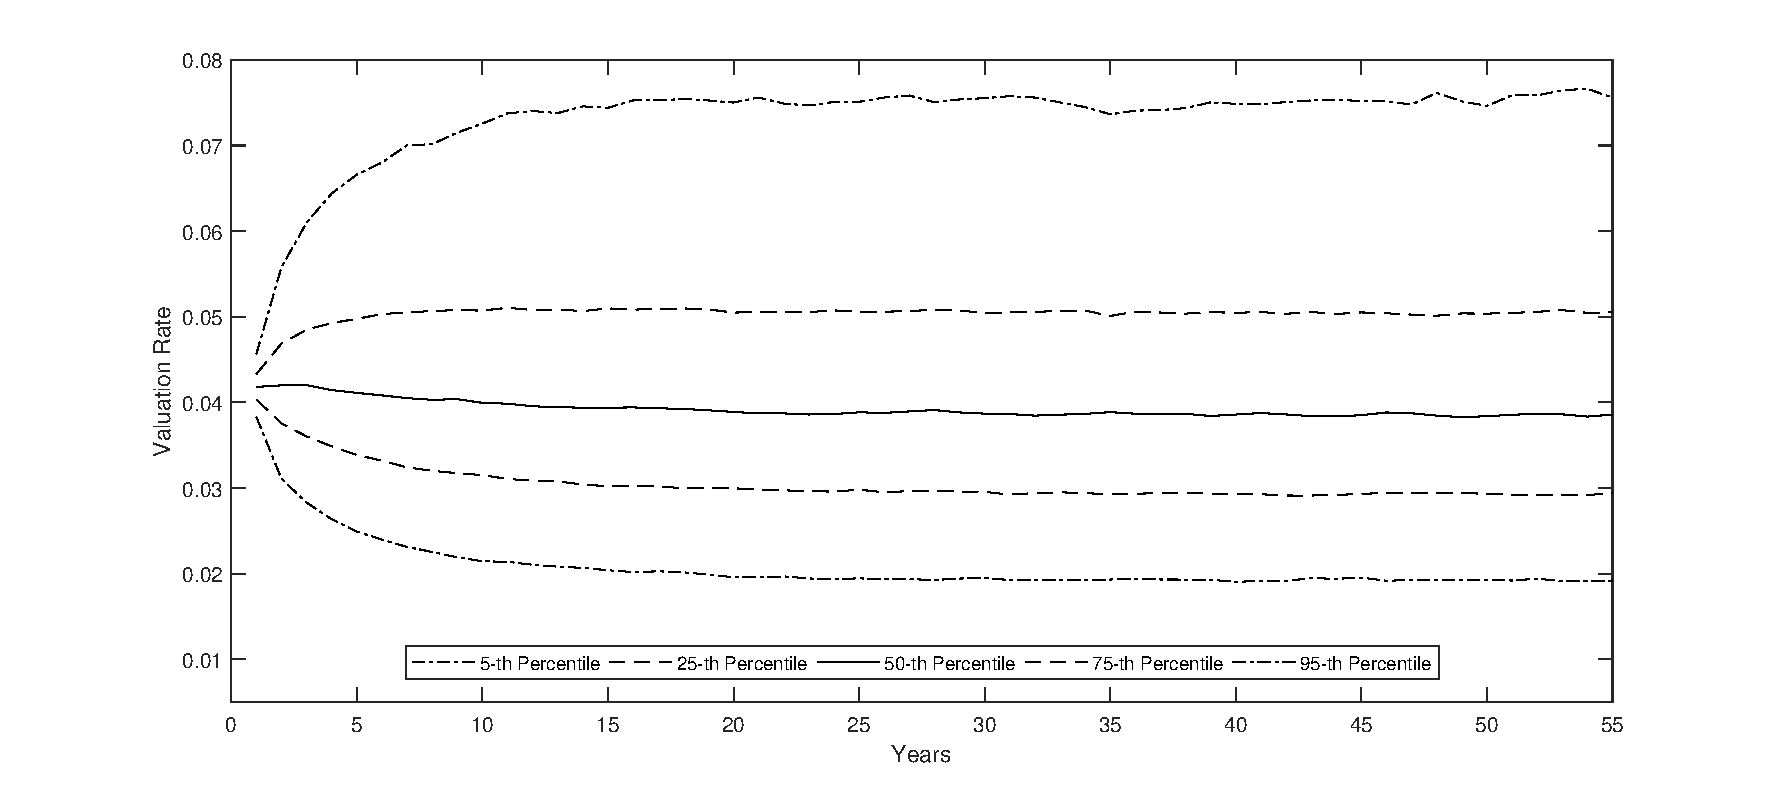
\includegraphics[width=\linewidth]{ResultPlot/DISC.pdf} 
			\caption[Funnel of Doubt for the Valuation Rate]{\textbf{Funnel of Doubt for the Valuation Rate}
				\vspace{-0.4cm}
				\newline\footnotesize\justify In the collective DC plan, long-term bond yields are used in the affordabiliy test to assess the plan liabilities. The $5^{\text{th}}$, $25^{\text{th}}$, $50^{\text{th}}$, $75^{\text{th}}$ and $95^{\text{th}}$ percentiles of the simulated distribution of the long-term bond yields are shown in the plot.}
			\label{fig:Funnel of Doubt for the Valuation Rate}
		\end{figure}
		\begin{figure}[h]
			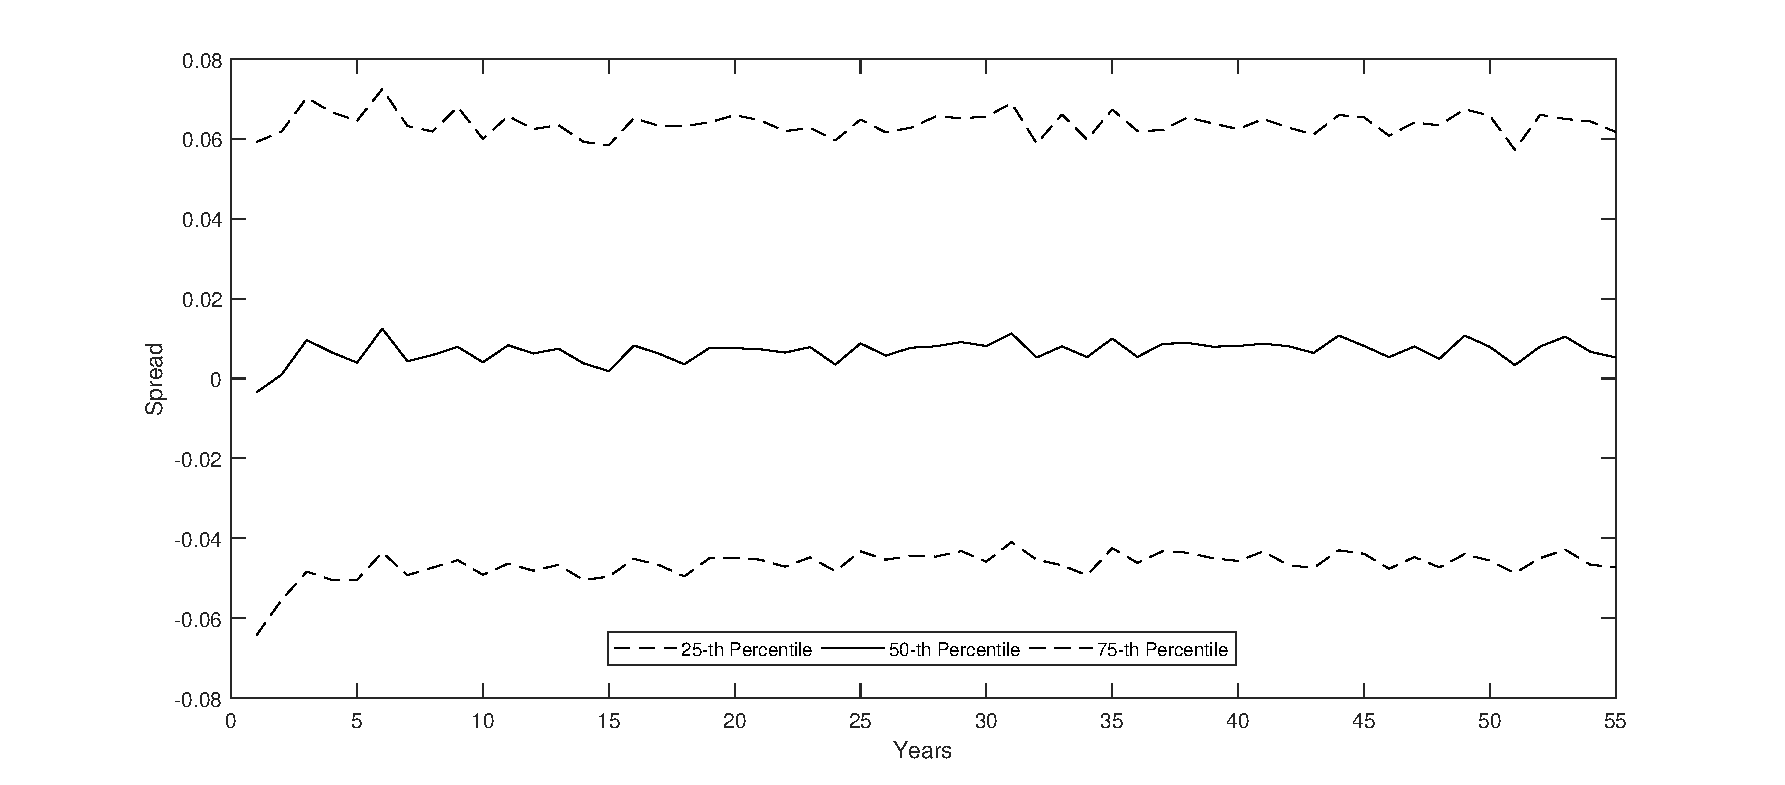
\includegraphics[width=1\linewidth]{ResultPlot/Spread.pdf} 
			\caption[Funnel of Doubt for the Spread Between Asset Return and Valuation Rate]{\textbf{Funnel of Doubt for the Spread Between Asset Return and Valuation Rate}
				\vspace{-0.4cm}
				\newline\footnotesize\justify The spread between asset return and valuation rate under each scenario is calculated by subtracting the valuation rate from the fund return. The $25^{\text{th}}$, $50^{\text{th}}$, and $75^{\text{th}}$ percentiles of the simulated spread distribution are shown in the plot.}
			\label{fig:Funnel of Doubt for the Spread Between Asset Return and Valuation Rate}
		\end{figure}
		\vspace{-0.4cm}
		
		\justify
		Since half of the plan assets are invested in the stock market, which earn equity risk premium in the long-run, the bond-based valuation rate tends to underestimate the investment return. Figure \ref{fig:Funnel of Doubt for the Spread Between Asset Return and Valuation Rate} shows the funnel of doubt for the asset return minus the valuation rate from the real-world economic scenarios (so-called spread). The median spread hovers around $1\%$, indicating that the fund is more likely to experience investment gains than losses.
	
	
		\justify
		The initial target annual accrual rate $b_{0}$ is $1\%$ as discussed in Section \ref{Target Benefit}. No immediate benefit adjustment is needed at time $0$ because the accrual rate is consistent with the affordability test.
	
	
		\justify
		The affordability test is performed once a year. A single trigger is applied and an action is taken to adjust the accrual rate $b_{t}$ immediately at each valuation based on the result of the test, if needed. Specifically, at each valuation time $t>0$, the new accrual rate $b_{t}$ is determined by adjusting the accrual rate $b_{t-1}$ established in the previous valuation by a factor $\alpha_{t}$.
	
	
		\justify
		One way to choose $\alpha_{t}$ would be such that the funded ratio after the adjustment is exactly $100\%$. In this case:
		
		\begin{equation}
		\label{eq:VB_added}
		\alpha_{t} = \frac{F_{t}}{PVTAB_{t} + PVTFB_{t} - PVFNC_{t}}
		\end{equation}
		and the new accrual rate would become 
		
		\begin{equation}
		\label{eq:VB_added2}
		b_{t} = \alpha_{t}b_{t-1}.				
		\end{equation}
		However, this setup led to considerable numerical instability in our simulations whenever the denominator of the expression for $\alpha_{t}$ above approached zero.
	
	
		\justify
		As an alternative, we implemented the following adjustment factor instead:
%		\begin{equation}
%		\label{eq:VB_2}
%		TAL_{t}^{*} = \alpha_{t} \, (PVTBP_{t} +PVTBF_{t}) - PVFNC_{t}.
%		\end{equation}
%		We denote the adjusted funded ratio at time $t$ by $FR_{t}^{*}$:
%		\begin{equation}
%		\label{eq:VB_3}
%		FR_{t}^{*} = \frac{F_{t}}{TAL_{t}^{*}}.
%		\end{equation}
%		To make the adjusted funded ratio $FR_{t}^{*}$ equal to $1$, $\alpha_{t}$ is calculated as
		\begin{equation}
		\label{eq:VB_4}
		\alpha_{t} = \frac{F_{t}+ PVFNC_{t}}{PVTAB_{t} + PVTFB_{t} }.
		\end{equation}
		Using this alternative, we have:
%		\begin{equation}
%		\label{eq:VB_5}
%		b_{t} = \alpha_{t}\, b_{t-1}.
%		\end{equation}
%		\vspace{-0.8cm}
		\begin{equation}
		\label{eq:VB_added3}
		\alpha_{t}(PVTAB_{t} + PVTFB_{t}) = F_{t} + PVFC_{t} - (PVFC_{t}-PVFNC_{t}),
		\end{equation}
		where
		\begin{itemize}
			\item The left-hand side is the present value of all benefits payable at or after time $t$, taking into account the adjustment at time $t$;
			\item $PVFC_{t}$ is the present value of future contributions, and $F_{t} + PVFC_{t}$ can be thought of as the present value of ``available assets'' at time $t$; and
			\item $PVFC_{t}-PVFNC_{t}$ is a countercyclical buffer that, when positive, reduces $\alpha_{t}$ by reducing the ``available assets.'' When this ``buffer'' is negative, it results in a larger $\alpha_{t}$.
		\end{itemize}
		
		\justify
		As stated in Section \ref{Target Benefit}, the actual annual benefit $B_{x,t}$ paid out to a retiree age $x$ at time $t$ is equal to $TB_{x,t}$ defined in Equation \eqref{eq:STBP_10}. Since there is no adjustment to the contributions under our collective DC plan, the annual contribution amount $C_{x,t}$ for an active member age $x$ at time $t$ remains $10.6\%$ of the salary $S_{x,t}$, as defined in Equation \eqref{eq:STBP_6}. 
	
	
	
		\justify
		The plan operations are projected for 55 years, so that the youngest already participating cohorts can receive their last benefit. The pension fund is assumed to be liquidated after $55$ years, and all the remaining assets are distributed to the participants as a lump sum payment at $t=55$, based on pre-defined entitlement criteria. 
	
	
		\justify
		We make a few observations about the performance of the plan using some of the metrics considered by \citet{Sanders2016a} before moving to the value-based ALM framework. Figure \ref{fig:Funnel of Doubt for the First Year Replacement Ratio by Valuation Year} shows the funnel of doubt for the first year replacement ratio and Figure \ref{fig:Distribution of Benefit Adjustments by Valuation Year} shows the distribution of benefit adjustments by size.
		\begin{figure}[H]
			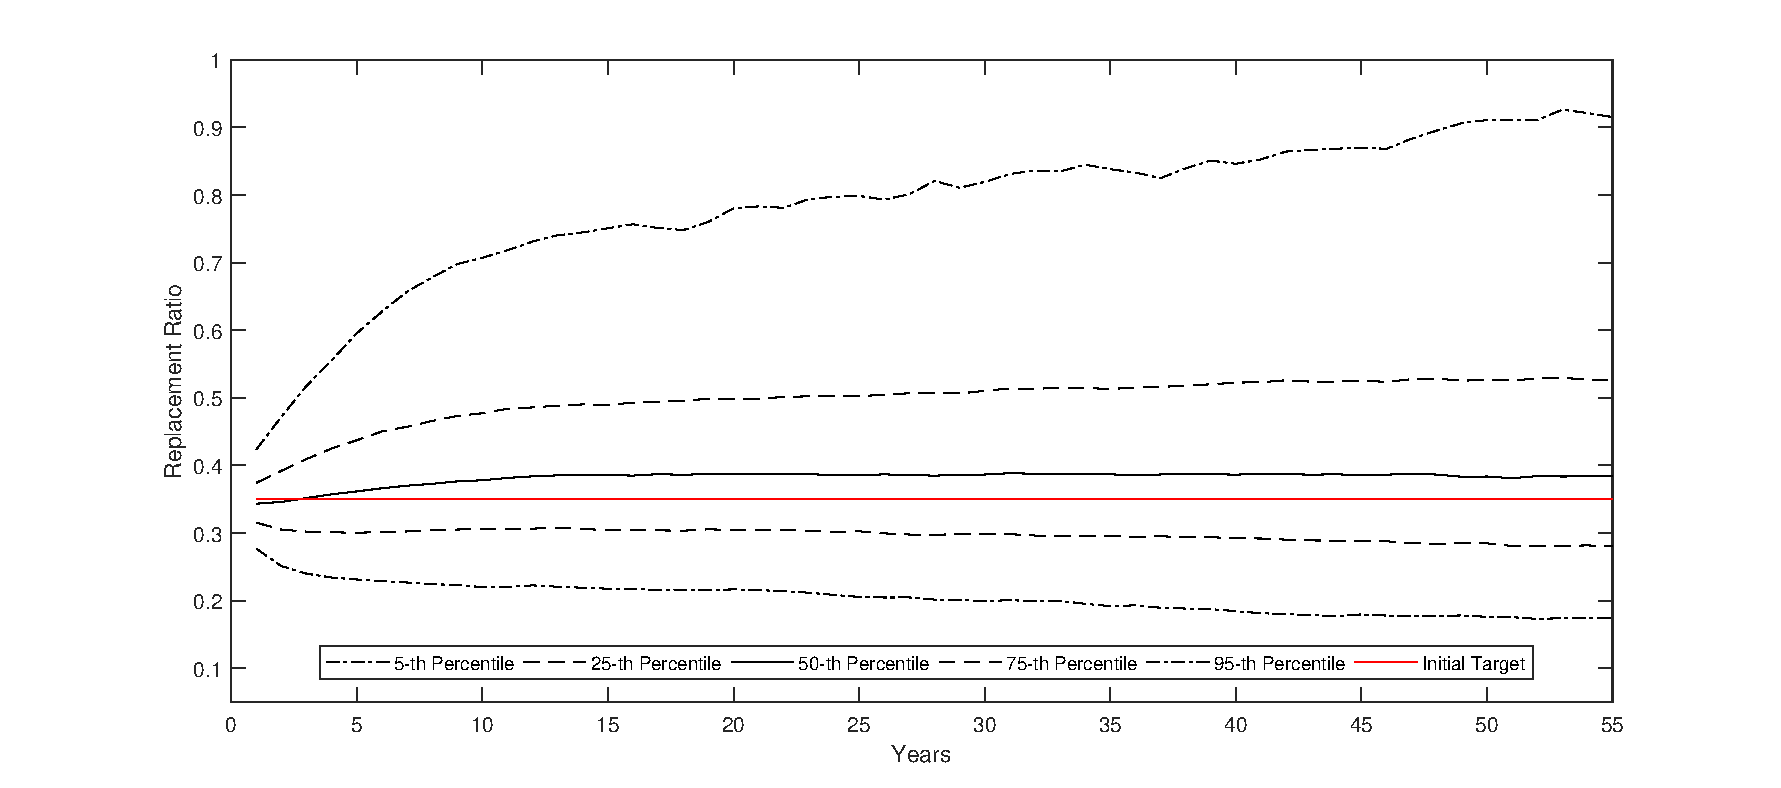
\includegraphics[width=1\linewidth]{ResultPlot/RR.pdf} 
			\caption[Funnel of Doubt for the First Year Replacement Ratio by Valuation Year]{\textbf{Funnel of Doubt for the First Year Replacement Ratio by Valuation Year}
				\vspace{-0.4cm}
				\newline\footnotesize \justify The first year replacement ratio for the new retired generation at year $t$ is calculated using Equation \eqref{eq:VB_6} under each scenario. This figure shows the $5^{\text{th}}$, $25^{\text{th}}$, $50^{\text{th}}$, $75^{\text{th}}$, and $95^{\text{th}}$ percentile of the simulated distribution of the first year replacement ratio over the $55$-year projection period.}
			\label{fig:Funnel of Doubt for the First Year Replacement Ratio by Valuation Year}
		\end{figure}
		
		\begin{figure}[h]
			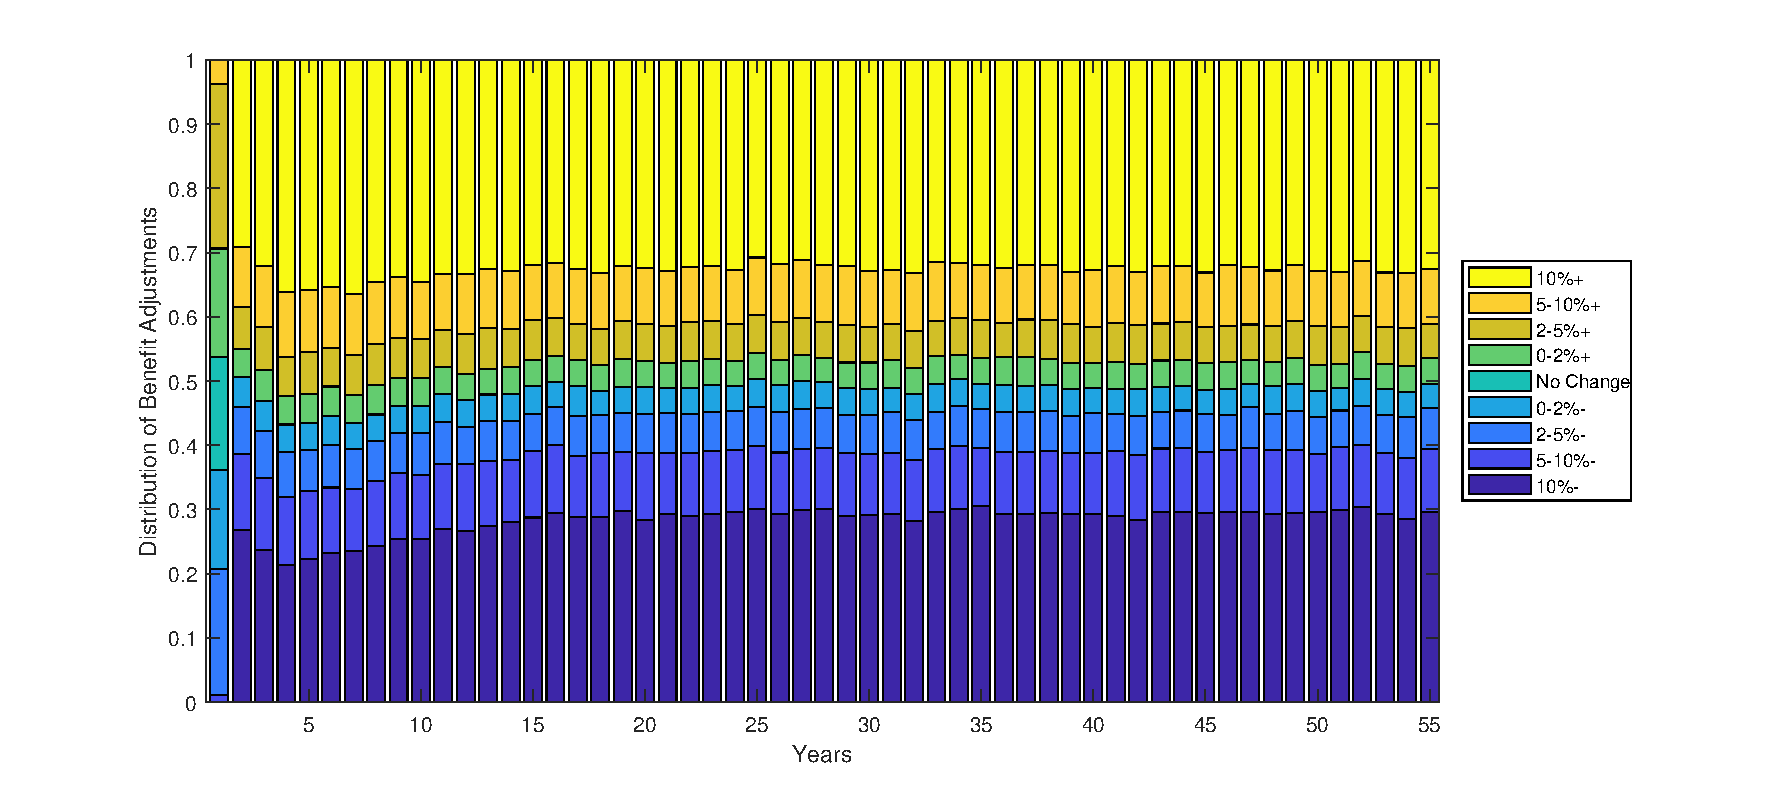
\includegraphics[width=1\linewidth]{ResultPlot/ProbIncDc.pdf} 
			\caption[Distribution of Benefit Adjustments by Valuation Year]{\textbf{Distribution of Benefit Adjustments by Valuation Year}
				\vspace{-0.4cm}
				\newline\footnotesize \justify The distribution of the size of the benefit adjustments is calculated at each valuation date. Each bar in the figure summarizes the distribution for a particular year.}
			\label{fig:Distribution of Benefit Adjustments by Valuation Year}	
		\end{figure}
		\vspace{-0.4cm}
		\justify
		The first year replacement ratio $RR_{t}$ for a generation that retires at time $t>0$ is calculated as
		\begin{equation}
		\label{eq:VB_6}
		RR_{t} = \frac{B_{r,t}}{S_{r-1,t-1}}.
		\end{equation}
		 Figure \ref{fig:Funnel of Doubt for the First Year Replacement Ratio by Valuation Year} shows that the plan has a median replacement ratio of $35\%$ at plan inception, which gradually increases to around $40\%$ after $10$ years. The horizontal line represents the replacement ratio based on the initial target accrual rate $b_{0}$. We can observe that the actual replacement ratio exceeds this initial target in more than half of the scenarios and for most of the generations.  
	
	
		\justify
		Figure \ref{fig:Distribution of Benefit Adjustments by Valuation Year} summarizes the distribution of benefit adjustments by size at each valuation date. Pensioners do not want their retirement benefits to fluctuate every year. However, since we use a single trigger in this plan, the benefits are not very stable: the probability of increasing or decreasing  the benefit drastically (i.e., by more than $10\%$) is quite high (about $50\%$). During the first five years of operations, the likelihood of large negative spreads between the portfolio return and the  valuation rate decreases (see Figure \ref{fig:Funnel of Doubt for the Spread Between Asset Return and Valuation Rate}). As a result, the downside benefit risk decreases during these years, which means that members are more likely to get positive benefit adjustments. This pattern can also be observed in Figure \ref{fig:Funnel of Doubt for the First Year Replacement Ratio by Valuation Year} as the distribution of the first year replacement ratio drifts upward in the early years of plan operations. Once the spread between the asset return and the valuation rate reaches its stationary level, the distribution of benefit adjustments also becomes stable with the probability of positive benefit adjustments hovering around $50\%$, and the median of the replacement ratio settling near $40\%$.
	
	
		\justify
		It is clear from these results that different cohorts of members face different distributions of risks and rewards. The value-based ALM framework allows us to investigate the fairness of these differences in terms of market-consistent value.
	
	
	\section{Generational Accounts}
	\label{Generational Accounts}
	
		\justify
		We use a generational account matrix to record all of the transactions for each cohort. The generational account matrix $\boldsymbol{GA^k}$, projected from time $0$ under a particular scenario $k$, can be depicted as follows:
		
		\begin{equation}
		\label{eq:VB_7}
		\left[
		\begin{array}{c:ccccccccc:c}
		0           &0 		       &0             &0             &\cdots & 0             &0             &\cdots  &0 			&C_{30,55}^{k}  &RV_{30,55}^k \\
		0           &0  	       &0 			  &0  			 &\cdots & 0 		  	 &0 			&\cdots  &C_{30,54}^{k} &C_{31,55}^{k}  &RV_{31,55}^k  \\
		\vdots      &\vdots 	   &\vdots 		  &\vdots  	     &       & \vdots 	     &\vdots 	    &        &\vdots 	    &\vdots         &\vdots \\
		0           &0  		   &C_{30,1}^{k}  &C_{31,2}^{k}  &\cdots & C_{63,34}^{k} &C_{64,35}^{k} &\cdots  &B_{83,54}^{k} &B_{84,55}^{k}  &RV_{84,55}^k \\
		0           &C_{30,0}^{k}  &C_{31,1}^{k}  &C_{32,2}^{k}  &\cdots & C_{64,34}^{k} &B_{65,35}^{k} &\cdots  &B_{84,54}^{k} &B_{85,55}^{k}  &0\\
		AVDC_{31,0} &C_{31,0}^{k}  &C_{32,1}^{k}  &C_{33,2}^{k}  &\cdots & B_{65,35}^{k} &B_{66,55}^{k} &\cdots  &B_{85,54}^{k} &0              &0 \\	
		\vdots      &\vdots 	   &\vdots 		  &\vdots  	     &       & \vdots 	     &\vdots 	    &        &\vdots 	    &\vdots         &\vdots  \\
		AVDC_{64,0} &C_{64,0}^{k}  &B_{65,1}^{k}  &B_{66,2}^{k}  &\cdots & 0 		     &0 		    &\cdots  &0 			&0              & 0 \\
		AVDC_{65,0} &B_{65,0}^{k}  &B_{66,1}^{k}  &B_{67,2}^{k}  &\cdots & 0 			 &0 		    &\cdots  &0             &0              &0 \\
		\vdots      &\vdots 	   &\vdots 		  &\vdots  	     &       & \vdots 	     &\vdots 	    &        &\vdots 	    &\vdots         &\vdots  \\
		AVDC_{84,0} &B_{84,0}^{k}  &0             &0  			 &\cdots & 0 			 &0             &\cdots  &0             &0              &0 \\
		AVDC_{85,0} &B_{85,0}^{k}  &0             &0  			 &\cdots & 0 			 &0             &\cdots  &0             &0              &0\\
		\end{array}
		\right].
		\end{equation}
	
	
		\justify
		In the generational account matrix, each row represents the generational account of a particular cohort, with the first row representing the youngest cohort who joins the plan at time $t=55$ and the last row representing the oldest cohort who is already $85$ years old at plan inception and has only one benefit to receive. 
	
	
		\justify
		Each column of the matrix represents a transaction date, corresponding to the beginning of each year. Under economic scenario $k$, the benefit received and the contribution paid by (or on behalf of) different cohorts are calculated. We assume that there are no investment costs or other expenses. In addition to the payments of contributions and benefits, there are two additional transactions: one at inception and the other at the termination of the pension plan. The former is the initial fund transfer from the individual DC plans made by generations older than 30, and the latter is the distribution of residual assets to the members who are still alive when the plan is terminated. 
	
	
		\justify
		The symbol $RV_{x,55}^k$ represents the amount of residual assets that are received by a member age $x$ at $t=55$ under scenario $k$. The total residual assets of the plan are distributed among members who are still alive, proportional to the actuarial liabilities $AL_{x,55}^{k}$ immediately after the transactions at $t=55$ take place, where
		\begin{equation}
		\label{eq:VB_8}
		AL_{x,55}^k = \left\{
		\begin{array}{ll}
		b_{55}^{k}\,(r\!-\!e) \, PFS^{k}_{x,55} \, \frac{\ddot{a}_{\angl{\omega\! -\! r }i^{V(k)}_{55}}}{(1\!+\!i^{V(k)}_{55})^{(r\!-\!x)}}\!-\! \alpha_{55}^{(k)}\, c_{x,55}^{NC(k)} \, S_{x,55}^k \, \ddot{a}_{\angl{r\! -\! x }i^{V(k)*}_{55}}\! +\! C_{x,55}^k &\text{ if } x<65 \\
		TB_{x,55}^{k}\, \ddot{a}_{\angl{\omega - x }i^{V(k)}_{55}} - B_{x,55}^{k} &\text{ if } x\geqslant 65\\
		\end{array}
		\right.,
		\end{equation}
		and the superscripts indicate values under scenario $k$. Then, the residual asset $RV_{x,55}^k$ received by a member age $x$ at $t=55$ can be expressed as
		\begin{equation}
		\label{eq:VB_9}
		RV_{x,55}^k = \left(F_{55}^k + \sum_{x} n_{x}C_{x,55}^k -\sum_{x} n_{x}B_{x,55}^k \right) \left( \frac{AL_{x,55}^{k}}{\sum_{x} n_{x} AL_{x,55}^{k} } \right).
		\end{equation}
	
	
		\justify
		The generational account matrix can be constructed under both the real-world scenarios and the risk-neutral scenarios. The real-world generational account value matrix shows the contribution and benefit payments that the plan member would expect under possible economic conditions in the future. The values of the benefits or contributions calculated under the risk-neutral scenarios are not meaningful in themselves, however, they enable us to calculate the market-consistent value of the pension deal for each generation at time $0$ and to investigate the gains and losses of each generation arising from their participation in the collective DC plan.
	
	
	\section{Value of the Pension Deal}
	\label{Value of the Pension Deal}
	
		\justify
		As discussed in Chapter \ref{Introduction}, the pension contract can be viewed as a combination of embedded options whose payoff is contingent on the market performance. Thus, the pension contract can be evaluated by employing option-valuation techniques. The fair market value at time $0$ of a future contingent payment can be calculated using risk-neutral valuation as defined in Equation \eqref{eq:ESG_8}. Having constructed the generational account matrix, we can calculate the generational pension value of each cohort under the collective DC plan. From the member's point of view, the initial fund transfer and the contributions are taken as negative cash flows, while the benefits and the residual value received at plan termination are considered as positive cash flows. We let
		\begin{itemize}
			\item $V_{x}$ be the value of the pension deal evaluated at $t=0$ for a member age $x$ at plan inception;
			% \item $GA_{x}$ be the contingent generational account for a member age $x$ at plan inception, which contains all the values of $AVDC_{x,0}$, $C_{x+t,t}$, $B_{x+t,t}$ and $RV_{x+55,55}$ throughout the life of this cohort, and $GA_{x}^{k}$ represents the outcome of $GA_{x}$ under scenario $k$;
			\item $Q_{t}^f$ be the $1$-period risk-free discount factor applicable to period $(t-1,t]$:
			\begin{equation}
			\label{eq:VB_10}
			Q_{t}^f = (1 + \tilde{r}_{t}^s)^{-1},
			\end{equation}
			and $Q_{0}^{f} = 1.$
		\end{itemize}
		The subscript $x$ in $V_{x}$ can range from $-25$ to $85$, with negative values of $x$ representing the cohorts that are not yet born at plan inception. According to Equation \eqref{eq:ESG_8}, the generational value of the pension deal under a collective DC plan can be calculated as the risk-neutral expected present value at $t=0$ of all cash flows in the generational account,
		\begin{equation}
		\label{eq:VB_11}
		V_{x} =
		\left\{
		\begin{array}{ll}
		\vspace{0.3cm}
		\E^{\mathbb{Q}}\!\left[\!-\!\sum\limits_{i=\!30\!-\!x}^{65\!-\!x\!-\!1}C_{x\!+\!i,i}\! \prod\limits_{j=\!0}^{i}Q_{j}^{f} \!+\!\sum\limits_{i=\!65\!-\!x}^{55}B_{x\!+\!i,i}\!\prod\limits_{j=\!0}^{i}Q_{j}^{f}\!  +\! RV_{x\!+\!55,55}\!\prod\limits_{j=\!0}^{55}Q_{j}^{f}\middle| \mathcal{F}_{0} \right] &\text{ if } x<30\\
		\vspace{0.3cm}
		\E^{\mathbb{Q}}\!\left[\! -AVDC_{x,0}\! -\! \sum\limits_{i=\!0}^{65\!-\!x\!-\!1}C_{x\!+\!i,i}\! \prod\limits_{j=\!0}^{i}Q_{j}^{f} +\sum\limits_{i=65\!-\!x}^{86\!-\!x}B_{x\!+\!i,i}\!\prod\limits_{j=0}^{i}Q_{j}^{f}\middle| \mathcal{F}_{0} \right] &\text{ if } 30\leqslant x<65\\
		
		\E^{\mathbb{Q}}\!\left[\!-AVDC_{x,0}\!+\!\sum\limits_{i=0}^{86\!-\! x}B_{x\!+i,i}\!\prod\limits_{j=0}^{i}Q_{j}^f \middle| \mathcal{F}_{0} \right] &\text{ if } x\geqslant 65\\
		\end{array}
		\right..
		\end{equation}
		\justify
		Practically speaking, the expected values are calculated by averaging over all risk-neutral scenarios. 
		\justify
		For members who have not yet joined the plan at inception, the value of the pension deal includes the value of the actual retirement benefits and the residual payout they will receive, less the  value of the contributions they will make. For active members at plan inception, the value of the deal is equal to the value of the retirement benefits they will receive net of the value of their initial contribution and all their future contributions. The retirees start receiving their retirement benefits immediately after plan inception and their pension value is equal to the value of the benefits they have yet to receive minus the initial contribution they made. 
	
	
        \justify
		Figure \ref{fig:Value of the CDC Plan for All Cohorts} shows the generational pension value for different cohorts under the collective DC plan. The values on the $x$-axis represent the ages at plan inception of the various cohorts who enter the plan before termination. Since the value of the pension deal is defined as the market value of all income payments minus all contributions, a pension value of $0$ represents a fair deal without any value transfers at plan inception. From Figure \ref{fig:Value of the CDC Plan for All Cohorts}, we see that the value of the pension deal for generations who are older than $25$ at inception is negative, meaning that these cohorts are expected to be net losers in value terms if they enter this collective DC plan. By contrast, the younger generations can expect to be net winners. It is important to note that, without access to any external funding sources, the pension deal is a zero-sum game in market value terms, so one cohort's gain comes at the expense of other cohorts.
	    \begin{figure}[h]
			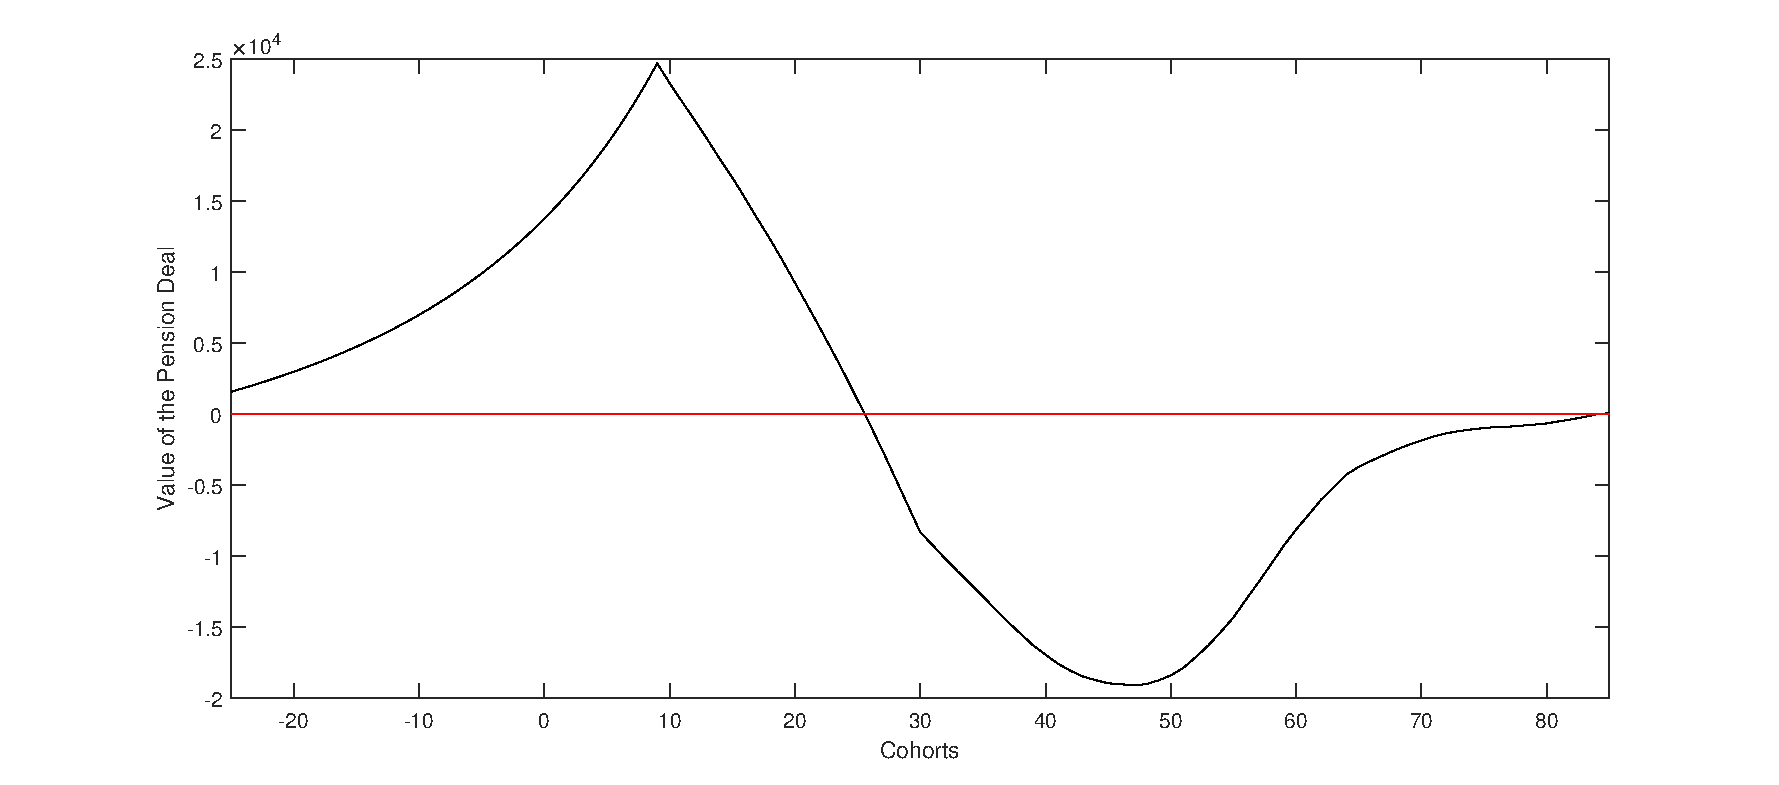
\includegraphics[width=1\linewidth]{ResultPlot/VPension.pdf} 
			\caption[Value of the Collective DC Plan for All Cohorts]{\textbf{Value of the Collective DC Plan for All Cohorts}
				\vspace{-0.4cm}
				\newline\footnotesize \justify The value of the pension deal is calculated using Equation \eqref{eq:VB_11} for all the generations who enter to the plan before termination. The $x$-axis in the figure shows all the cohorts of members, with negative numbers representing the cohorts who are not yet born at plan inception.}
			\label{fig:Value of the CDC Plan for All Cohorts}
		\end{figure}
	
	\vspace{-0.4cm}
	
		\justify
		The resulting shift in value is significant: the cohort that is worst off (those around age 47 at plan inception) loses nearly $\$20{,}000$ in value ($37\%$ of their salary at inception), whereas those who are best off gain about $\$25{,}000$. Although this plan does not have explicit risk sharing, Figure \ref{fig:Value of the CDC Plan for All Cohorts} draws attention to the implicit risk-sharing structure of the collective DC plan. The collective DC plan includes both active members who are paying contributions and retirees who have already received benefits from the plan. The benefits of these two groups of participants are subject to different types of risks. For example, inflation experience will have a direct impact on the salaries of active members which will affect their projected benefits but would not normally affect the retirees' benefits. However, since the decisions regarding benefit adjustments are made by reference to the experience of the whole plan with no distinction between cohorts, all risks including inflation risk, valuation rate risk and investment risk are shared implicitly among all the members. 
	
		\justify
		One significant cause of value transfers in our collective DC plan is the use of valuation rates based on bond yields. As discussed in Section \ref{CDC Plan Operations}, this often leads to the investment return being underestimated, which results in overestimating the plan liabilities and underestimating the funded ratios. Therefore, the benefit payments to retirees are generally lower than the fair amount. A portion of the investment gains on assets are retained in the plan and these extra savings will not be paid out until the plan is terminated. At plan termination, the extra savings are distributed to the remaining generations in proportion to their final actuarial liabilities. Thus, the generation with the highest actuarial liabilities will receive the greatest benefit from these extra assets, which is the generation aged $9$ at plan inception (age $64$ at plan termination). 
	
	
	
	\section{Decomposition of Risk Sharing into Call and Put Options}
	\label{Surplus and Deficit Options}
	
		\justify
		In this section, we explore how much risk each generation shares with other plan members. We cast the additional risks assumed by each generation as call and put options, so the price or value of bearing these extra risks can be calculated as the value of the corresponding options.
	
		\justify
		Inspired by \citet{Kocken2006} and \citet{soer2012}, we decompose the value of the pension deal determined in the previous section into:
		\begin{itemize}
			\item The pension value under some benchmark plan;
			\item The value of embedded options written on top of the benchmark plan, that are implicit in the collective DC plan.
		\end{itemize}
	
		\justify
		The benchmark plan and the embedded options can be selected in different ways depending on the focus of interest. In papers investigating the Dutch pension reforms, such as \citet{Kocken2006}, the DB plan is selected as the benchmark, since his focus was on how much risk is transferred to plan members during the transition from a DB plan to a TBP. 
	
	
		\justify
		In this research, we want to investigate the value transfers caused by entering a collective DC plan with implicit risk-sharing elements. Consequently, we choose an individual DC plan as our benchmark. Since this benchmark does not involve any risk-sharing, the difference in value between this benchmark and our collective DC plan can be interpreted as relating to risk sharing. For this comparison to be meaningful, the individual DC plan should have the same level of funding as the collective DC plan, including initial assets, contributions, and the same investment portfolio. 
	
	
	\subsection{Individual DC Plan Benchmark}
	\label{Individual Defined Contribution Plan}
	
		\justify
		We simulate the operation of an individual DC plan to create a benchmark. Under the individual DC plan, instead of joining the collective fund, each member continues to contribute to her own individual savings account and the benefits are paid from this savings account based on a selected decumulation strategy after retirement. There are many choices for the decumulation strategy and different choices will lead to different benefit payout patterns under the individual DC plan, which then affect the value of the embedded options. In this research, we use a bond-based decumulation strategy in which the benefits payable at the beginning of each year are calculated as the payouts deemed to be ``affordable'' for the given individual, taking into account their current individual DC account balance, their remaining lifetime, and prevailing yields on 15-year zero coupon bonds. We let
		\begin{itemize}
			\item $AVDC_{x,t}$ be the individual DC account value of a plan member age $x$ at time $t$ ($t>0$);
			\item $B^{'}_{x,t}$ be the annual retirement benefit drawn from the individual DC account by a member age $x$ at time $t$, where $x \geqslant 65$.
		\end{itemize}
		This retirement benefit is expressed as
		\begin{equation}
		\label{eq:VB_12}
		B^{'}_{x,t} = \frac{AVDC_{x,t}}{\ddot{a}_{\angl{\omega -x}\tilde{r_{t}}^{l}}}.
		\end{equation}
		Given that the starting account value at time $0$, the contribution rate and returns on assets are the same for the individual DC plan as they were under the collective DC plan, we can calculate the individual DC account value at time $t$ for a member age $x$ recursively as
		\begin{equation}
		\label{eq:VB_13}
		AVDC_{x,t} =
		\left\{
		\begin{array}{ll}
		
		(AVDC_{x-1,t-1} + C_{x-1,t-1})\, (1+r_{t}^P) &\text{ if } x<65\\
		
		(AVDC_{x-1,t-1} - B_{x-1,t-1}^{'})\, (1+r_{t}^P) &\text{ if } x\geqslant 65\\
		\end{array}
		\right..
		\end{equation}
	
		\justify
		Since both the returns on assets and the bond yields vary by scenario, the individual DC plan outcomes are also scenario dependent. For each scenario $k$, we can construct the generational accounts matrix of the individual DC plan $\boldsymbol{GADC^{k}}$ in the same form as $\boldsymbol{GA^{k}}$:
		
		\begin{equation}
		\label{eq:VB_14}
		\left[
		\begin{array}{c:ccccccccc:c}
		0           &0 		       &0             &0             &\cdots & 0             &0             &\cdots  &0 			&C_{30,55}^{k}  &RV_{30,55}^{'k} \\
		0           &0  	       &0 			  &0  			 &\cdots & 0 		  	 &0 			&\cdots  &C_{30,54}^{k} &C_{31,55}^{k}  &RV_{31,55}^{'k}  \\
		\vdots      &\vdots 	   &\vdots 		  &\vdots  	     &       & \vdots 	     &\vdots 	    &        &\vdots 	    &\vdots         &\vdots \\
		0           &0  		   &C_{30,1}^{k}  &C_{31,2}^{k}  &\cdots & C_{63,34}^{k} &C_{64,35}^{k} &\cdots  &B_{83,54}^{'k} &B_{84,55}^{'k}  &RV_{84,55}^{'k} \\
		0           &C_{30,0}^{k}  &C_{31,1}^{k}  &C_{32,2}^{k}  &\cdots & C_{64,34}^{k} &B_{65,35}^{'k} &\cdots  &B_{84,54}^{'k} &B_{85,55}^{'k}  &0\\
		AVDC_{31,0} &C_{31,0}^{k}  &C_{32,1}^{k}  &C_{33,2}^{k}  &\cdots & B_{65,35}^{'k} &B_{66,55}^{'k} &\cdots  &B_{85,54}^{'k} &0              &0 \\	
		\vdots      &\vdots 	   &\vdots 		  &\vdots  	     &       & \vdots 	     &\vdots 	    &        &\vdots 	    &\vdots         &\vdots  \\
		AVDC_{64,0} &C_{64,0}^{k}  &B_{65,1}^{'k}  &B_{66,2}^{'k}  &\cdots & 0 		     &0 		    &\cdots  &0 			&0              & 0 \\
		AVDC_{65,0} &B_{65,0}^{'k}  &B_{66,1}^{'k}  &B_{67,2}^{'k}  &\cdots & 0 			 &0 		    &\cdots  &0             &0              &0 \\
		\vdots      &\vdots 	   &\vdots 		  &\vdots  	     &       & \vdots 	     &\vdots 	    &        &\vdots 	    &\vdots         &\vdots  \\
		AVDC_{84,0} &B_{84,0}^{'k}  &0             &0  			 &\cdots & 0 			 &0             &\cdots  &0             &0              &0 \\
		AVDC_{85,0} &B_{85,0}^{'k}  &0             &0  			 &\cdots & 0 			 &0             &\cdots  &0             &0              &0\\
		\end{array}
		\right],
		\end{equation}
		where $RV_{x,55}^{'}$ represents the lump sum payment at plan termination to a member age $x$. This payout is simply the balance in the member's individual DC account at that time, i.e., $AVDC_{x,55}$. The generational value of the individual DC plan $V_{x}^{'}$ is calculated as the risk-neutral expected present value of all cash flows in the generational account at $t=0$ similar to Equation \eqref{eq:VB_11}.
	
	
		\justify
		The generational value of the individual DC plan is $0$ for all cohorts, which means that the market value of the benefits received by each generation is exactly the same as the value of the contributions made to the fund. This confirms the idea that the individual DC plan is self-financed and there are no value transfers among generations.
	
	
	\subsection{Embedded Options}
	\label{Embedded Options}
	
		\justify
		As discussed at the beginning of Section \ref{Surplus and Deficit Options}, the starting account balance and subsequent contributions are the same under the individual DC benchmark as they are under the collective DC plan. However, the benefits paid to retirees under the collective DC plan may differ from those under the individual DC benchmark, since the former adjusts the benefits of each member by reference to the experience of the whole plan. In effect, by joining the collective DC plan, the participants write put options to the plan, which waive part of the benefits they would get in the individual DC plan under certain economic conditions. The put options give a right to the plan and impose an obligation on the participants. Generally, an option writer will receive an option premium in return for bearing a risk; however, these put options are ``embedded'' in the pension contract and not explicitly sold as financial products, thus no option premium is paid to the participants as compensation for bearing the risk. Instead, participants are offered call options written on the fund surplus. The same applies to the residual asset under the collective DC plan: it can be thought of as the residual asset under the individual DC plan plus a put option written by members and a call option received by members. This gives us four kinds of options: a benefit put option, a benefit call option, a residual put option and a residual call option. 
		
		\begin{itemize}
			\item The \textit{benefit put option} is a basket of options that the participants write to the pension plan. These options expire at consecutive benefit payment dates starting with $t=1$. The payoff of a benefit put option expiring at time $t$ written by a member age $x$ at plan inception is defined as
			\begin{equation}
			\label{eq:VB_15}
			BP_{x,t} = \max(B_{x+t,t}^{'} - B_{x+t,t}, 0).
			\end{equation}
			The option is in-the-money when $B_{x,t}^{'} > B_{x,t}$. 
			
			\item The \textit{benefit call option} is a basket of options that the plan writes to the participants, expiring at each consecutive benefit payment date. The payoff of a benefit call option expiring at time $t$ written to a member age $x$ at plan inception is defined as
			\begin{equation}
			\label{eq:VB_16}
			BC_{x,t} = \max(B_{x+t,t} - B_{x+t,t}^{'}, 0).
			\end{equation}
			The option is in-the-money when $B_{x,t} > B_{x,t}^{'}$. This option is the ``opposite'' of the benefit put option. Together, these two (baskets of) options capture the deviations of the retirement benefits under the collective DC plan compared to the individual DC benchmark.
			
			\item The \textit{residual put option} is a basket of options that the participants write to the pension plan, expiring at $t= 55$. The payoff of the residual put option written by a member age $x$ at plan inception is defined as
			\begin{equation}
			\label{eq:VB_17}
			RP_{x} = \max(RV^{'}_{x+55,55} - RV_{x+55,55},0).
			\end{equation}
			At the termination of the pension plan, there are still generations who have not received their full benefits and generations who are not yet retired. These generations can make claims on the fund's residual wealth. The value of the assets that are left in the group fund depends on how much is spent on the benefits of the members who have already retired. For generations who are still active at the plan termination date, the residual asset they get is not necessarily equal to the accumulated value of the contributions they already made, which is the residual payment they would get under the benchmark individual DC plan. When this option is in-the-money, it implies that some of the benefits received by the already retired generations are at the expense of the future generations. 
			
			\item The \textit{residual call option} is a basket of options that the pension plan writes to the participants, expiring at $t=55$. The payoff of the residual call option written by the pension plan to a member age $x$ at plan inception is defined as
			\begin{equation}
			\label{eq:VB_18}
			RC_{x} = \max(RV_{x+55,55} - RV^{'}_{x+55,55},0).
			\end{equation}
			This option is the ``opposite'' of the residual put option. When it is in-the-money, it implies that additional funds are left over for future generations above and beyond what they would be entitled to under the individual DC benchmark.
		\end{itemize}
	
	
		\justify
		Since the benefits and residual values of both the collective DC plan and the individual DC plan are scenario dependent, all four of these options are Margrabe options. Introduced by \citet{Margrabe1978}, these options exchange one risky asset for another at maturity. The value of these options at time $0$ can be calculated using the risk-neutral valuation technique as 
		\begin{align}		
		VBP_{x,t} = &\, \E^{\mathbb{Q}} \left[\max(B_{x+t,t}^{'}-B_{x+t,t},0)\prod_{j=0}^{t}Q_{j}^f \middle|\mathcal{F}_{0} \right], \label{eq:VB_21}\\
		VBC_{x,t} = &\, \E^{\mathbb{Q}} \left[\max(B_{x+t,t}-B_{x+t,t}^{'},0)\prod_{j=0}^{t}Q_{j}^f \middle|\mathcal{F}_{0} \right], \label{eq:VB_22}\\
		VRP_{x} = &\,\E^{\mathbb{Q}} \left[\max(RV_{x+55,55}^{'}-RV_{x+55,55},0)\prod_{j=0}^{55}Q_{j}^f \middle|\mathcal{F}_{0} \right], \label{eq:VB_23}\\
		VRC_{x} = &\,\E^{\mathbb{Q}} \left[\max(RV_{x+55,55}^{'}-RV_{x+55,55},0)\prod_{j=0}^{55}Q_{j}^f \middle|\mathcal{F}_{0} \right].
		\label{eq:VB_24}
		\end{align}
		\justify
		The value of the total benefit put option $VTBP_{x}$ for a member age $x$ at plan inception is the aggregate value of all the benefit put options written by the member. It is equal to $0$ for cohorts who are still active at plan termination (i.e., less than age $10$ at plan inception) and it is equal to
		\begin{equation}
		\label{eq:VB_19}
		VTBP_{x} = \sum_{t=\max(65-x,0)}^{55} VBP_{x,t}
		\end{equation}
		for other generations. 
	
	
		\justify
		The value of the total benefit call option $VTBC_{x}$ for a member age $x$ at plan inception is calculated similarly:
		\begin{equation}
		\label{eq:VB_20}
		VTBC_{x} = \left\{
		\begin{array}{ll}
		0 &\text{ if } x<10\\
		\sum\limits_{t=\max(65-x,0)}^{55} VBC_{x} &\text{ if } x\geqslant 10\\
		\end{array}
		\right..
		\end{equation}
	
	
		\justify
		For generations younger than 10 years old at plan inception, the value of the options written on the benefit payouts are $0$, thus the gain or loss in value triggered by joining the collective DC plan is reflected in the value of the residual options only.
	
	
		\justify
		Figure \ref{fig:Surplus and Deficit Options} shows the value of the options embedded in the collective DC plan for all cohorts. From the benefit options plot (top panel), we can observe that most cohorts have significant upside potential as measured by $VTBC$ (up to $\$30{,}000$ in market value terms), but this is more than offset by the downside potential, as measured by $VTBP$. This is because we use the bond-based valuation rates in the collective DC plan. As discussed in Section \ref{Value of the Pension Deal}, using the conservative valuation rate results in lower benefit payments to retirees than what they should get. The problem is worse for the cohorts age $30$ to $65$ at plan inception, who get all their retirement benefits paid out during the life of the plan, because of more exposure to the value transfers. As we discussed in Section \ref{Generational Accounts}, the extra assets held back by the plan are distributed at plan termination to the generations who are still in the plan at that time. This is consistent with the results in the residual options plot (middle panel), where the $VRC$ is much greater than $VRP$. The generation who is 9 years old at plan inception is the oldest active cohort at plan termination and has the highest actuarial liability at that point. As a result they get the biggest portion of the residual assets and have the highest $VRC$. 
		\begin{figure}[h]
			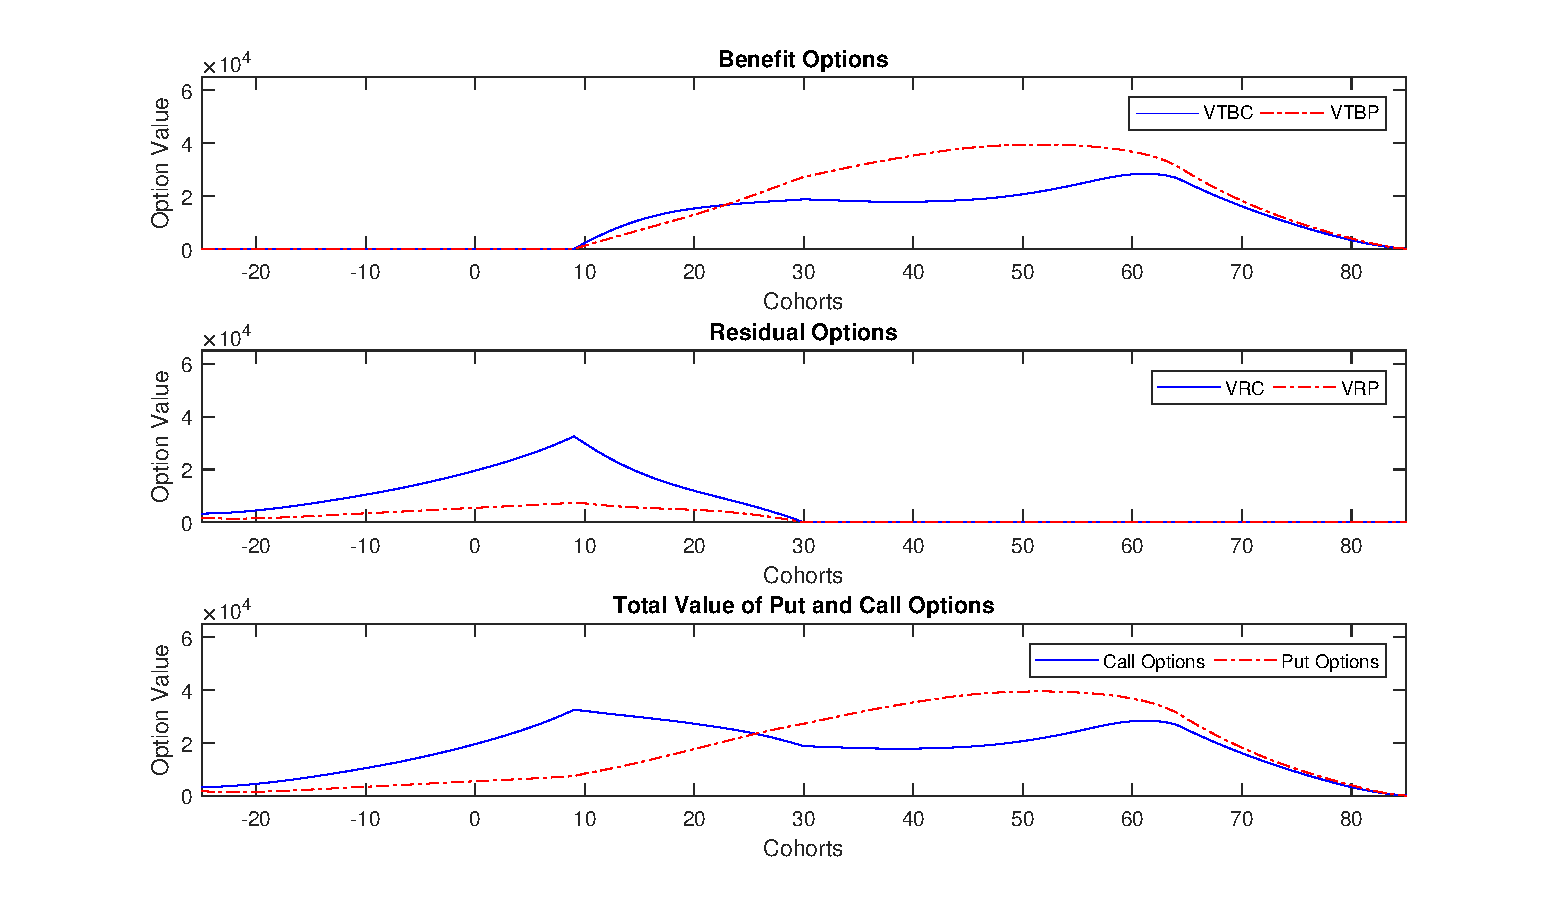
\includegraphics[width=1\linewidth]{ResultPlot/SDOptions.pdf} 
			\caption[Embedded Options in Collective DC Plan Relative to Individual DC Benchmark]{\textbf{Embedded Options in Collective DC Plan Relative to Individual DC Benchmark}
				\vspace{-0.4cm}				
				\newline\footnotesize\justify The value of the embedded options are calculated for all the generations who enter to the plan before plan termination. The figure on the top shows the generational values of $VTBC$ and $VTBP$ calculated using Equations \eqref{eq:VB_19} and \eqref{eq:VB_20}. The figure in the middle shows the generational values of $VRC$ and $VRP$ calculated using Equations \eqref{eq:VB_23} and \eqref{eq:VB_24}. The figure at the bottom shows the total value of the call options and the put options for each generation. The $x$-axis in the figure shows all the cohorts of members and the negative numbers represents the cohorts who are not born at plan inception. }
			\label{fig:Surplus and Deficit Options}
	\end{figure}
	
	
		\justify
		If the plan kept operating past $t=55$, the residual options would disappear. As a result, the younger generations who are expected to be net winners under the current setting would no longer expect to have such a large advantage.
	
	
		\justify
		The third panel in Figure \ref{fig:Surplus and Deficit Options} shows the aggregate value of the surplus options and deficit options from the first two plots. Since the value of the individual DC plan is equal to $0$ for each generation, the value of the pension deal for each cohort is equal to the total value of the call options of that cohort less the total value of the put options for the same cohort.
	
	
	\section{Key Findings}
	\label{Key Findings}
	\justify
	In this chapter, we analyze the generational value of a simple collective DC plan using the value-based ALM approach. Under our collective DC plan, there are no intertemporal benefit smoothing designs being implemented. Therefore, the retirement benefits fluctuate a lot. The benefits are adjusted every year and half of the time they change by more than $10\%$. This is a very simplistic design, not reflective of TBPs in practice; however, it allows us to demonstrate two important features (implicit risk sharing and the impact of bond-based valuation rates), which may be difficult to see in more complex designs.
	
	\justify
	To recap, although there are no intentional inter-generational subsidies built into this plan design, value transfers among different cohorts are still significant. One of the reasons for this is the implicit risk sharing in the collective pension scheme. At any time during the simulation period, there are active members who are still earning benefits and paying contributions as well as retirees who are already receiving benefits from the plan. As discussed in Section \ref{Value of the Pension Deal}, these two groups of participants are subject to different types of risks. Even within each group, the impact of changes in the inflation rate and the valuation rate is not the same for all cohorts of members, because the amount of retirement savings and the duration of the pension liabilities are different. However, under our collective DC plan, the target benefits in respect of both past and future service are adjusted simultaneously each year based on the funded position of the whole plan, without distinguishing between different generations. Therefore, the inflation and valuation rate risks are shared implicitly among generations, giving rise to part of the value transfers.
	
	
	\justify
	Another significant cause of value transfers in our collective DC plan is the use of valuation rates based on bond yields. This conservative valuation assumption does not take into account the market risk premium expected to be earned on half of the plan assets invested in equities. The plan liabilities are constantly overestimated, which leads to lower funded ratios thus lower retirement benefits than otherwise. As a result, more assets are retained in the plan. These extra assets are distributed at plan termination to the remaining generations in proportion to their final actuarial liabilities. Therefore, the generations who are still in the plan at termination are expected to be winners under this circumstance. The generation with the highest actuarial liabilities will receive the greatest benefit, which is the generation aged $9$ at plan inception (age $64$ at plan termination).
	
	\justify
	Since there are no external guarantees from the plan sponsors, the pension deal is a zero-sum game across all generations from the market value perspective. This is consistent with the conclusions in \citet{Cui2011}. It means that the surplus of one group of members comes at the expense of another group. In our case, the generations who are younger than $25$ years old at plan inception are expected to be net winners. Most of their surplus results from the fund distribution at plan termination, which is at the expense of smaller retirement benefits paid to older generations.
	
	\chapter{Inter-generational Impact of Key Design Choices}
	\label{Comparisons of Different TBP Plan Designs}
	The relationship between inter-generational equity and key design choices in TBPs is of great concern to actuaries and other stakeholders. One area of particular interest and active debate is the choice of valuation rate (i.e., bond-based or expected return on assets (EROA)) and its inter-generational impact. Another important question is related to the potential value transfers arising from adding mechanisms designed to stabilize benefits, such as introducing two trigger points to create a no-action range. In both cases, practitioners are generally aware of the direction of inter-generational value transfers, but not necessarily their size. Our goal is to enhance stakeholders' understanding by quantifying the impact of key design elements on inter-generational equity using the value-based ALM approach. 
	
	\section{TBP Designs with Different Valuation Rate Assumption}
	\label{TBP Designs with Different Valuation Rate Assumption}

		\justify
		The collective DC plan analyzed in Chapter \ref{Value-Based ALM Study of a Collective Defined Contribution Plan} uses a bond-based valuation rate in the affordability tests. Using the EROA as the valuation rate (effectively anticipating the equity risk premium) is permitted under Canadian pension regulations. We conjecture that using the EROA in liability valuation will create different patterns of generational outcomes than using the bond-based valuation rate. \citet{Sanders2016a} has investigated the changes in the dynamics of the retirement benefits after applying EROA as the valuation rate. \citet{Ma2018} also explored the issue of selecting discount rates for assessing the funded status of target benefit plans and concluded that a valuation rate based on EROA is more equitable and serves the best interests of all members. We are interested in testing the conclusion of \citet{Ma2018} under our framework. In this section, we change the valuation rate to the EROA as defined in Equation \eqref{eq:STBP_20}, while all other design factors remain the same. Figure \ref{fig:Funnel of Doubt of Valuation Rate in EROA Plan} shows the funnel of doubt of the new valuation rate.
		\begin{figure}[h]
			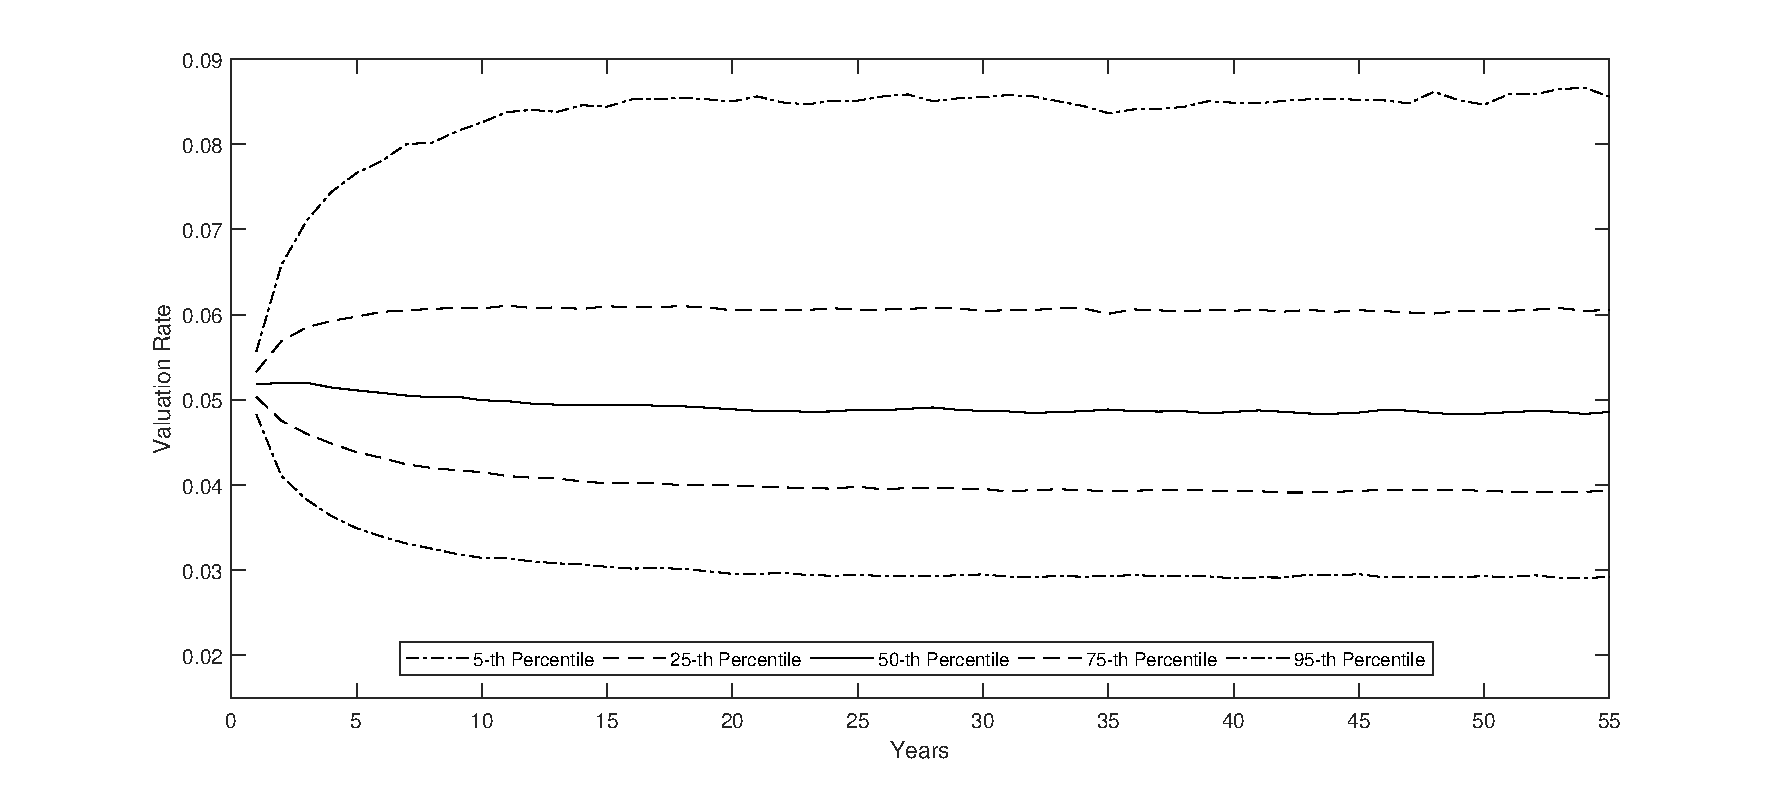
\includegraphics[width=\linewidth]{ResultPlot/DISC1.pdf} 
			\caption[Funnel of Doubt of Valuation Rate in EROA Plan]{\textbf{Funnel of Doubt of Valuation Rate in EROA Plan}
			\vspace{-0.4cm}
			\newline\footnotesize\justify EROA is calculated using Equation \eqref{eq:STBP_20} and it is used in the affordability tests to assess the plan liabilities. The $5^{\text{th}}$, $25^{\text{th}}$, $50^{\text{th}}$, $75^{\text{th}}$ and $95^{\text{th}}$ percentiles of the simulated distribution of the EROA are shown in the plot.}
			\label{fig:Funnel of Doubt of Valuation Rate in EROA Plan}
		\end{figure}

		\justify
		Compared with the bond-based valuation rate in Figure \ref{fig:Funnel of Doubt for the Valuation Rate}, the entire distribution of the new valuation rate is shifted up by about $1.1\%$, as anticipated from Equation \eqref{eq:STBP_20}. Since the asset mix is the same as under the collective DC plan in Chapter \ref{Value-Based ALM Study of a Collective Defined Contribution Plan}, the asset return dynamics are also the same. Figure \ref{fig:Funnel of Doubt of the Spread between Asset Return and Valuation Rate in EROA Plan} shows the funnel of doubt of the spread between the asset return and the valuation rate using EROA. After reaching its stationary level, the median of the distribution of the valuation spread is close to zero.
		\begin{figure}[H]
			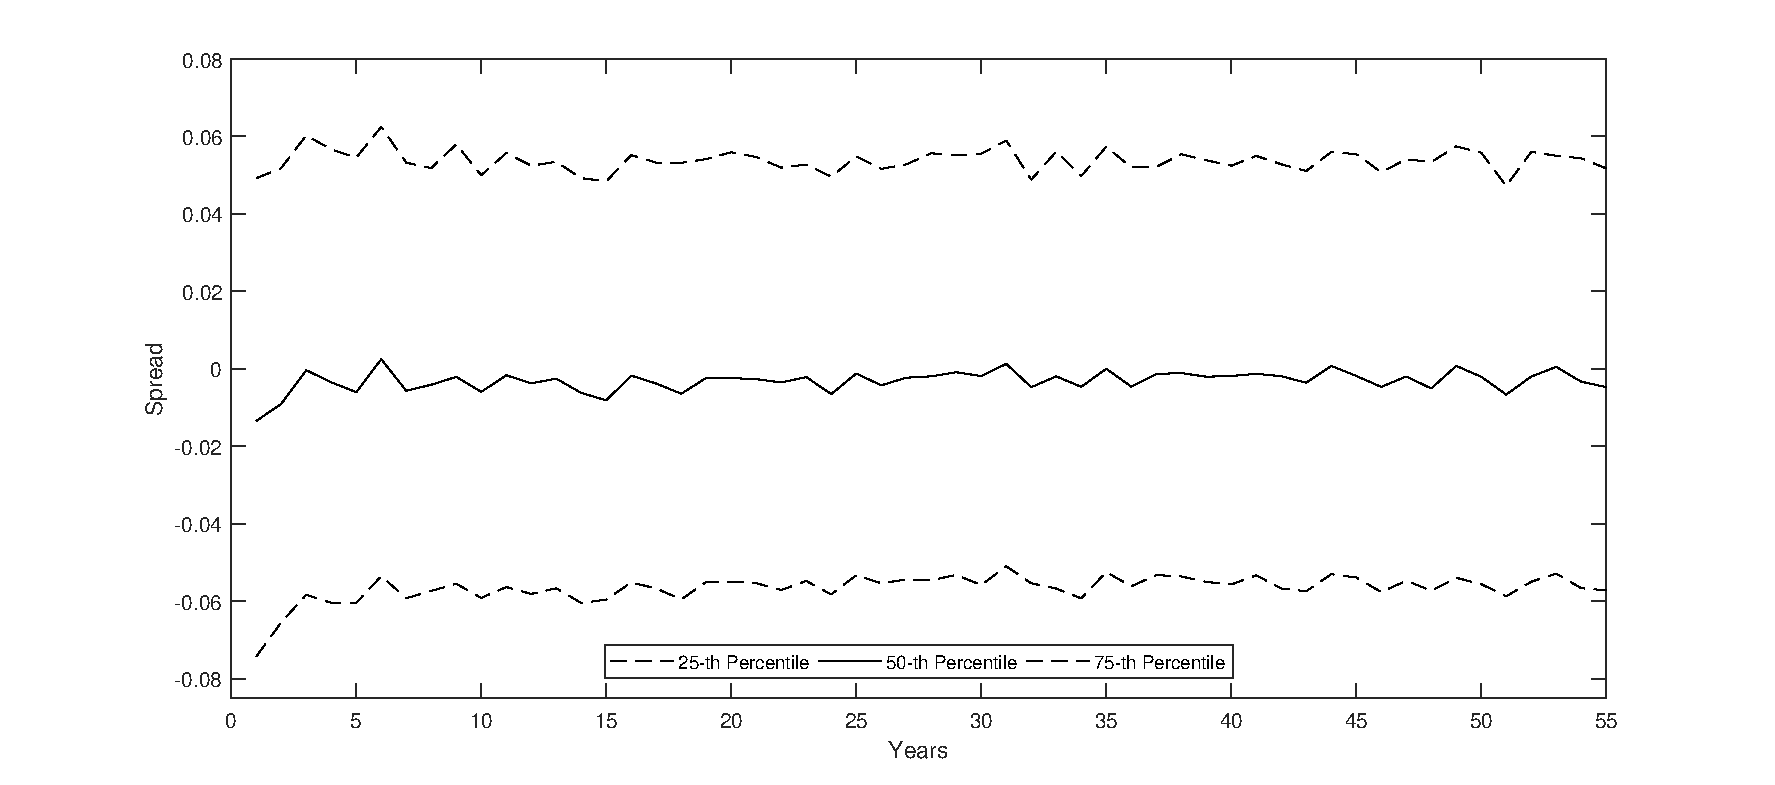
\includegraphics[width=1\linewidth]{ResultPlot/Spread1.pdf} 
			\caption[Funnel of Doubt of the Spread between Asset Return and Valuation Rate in EROA Plan]{\textbf{Funnel of Doubt of the Spread between Asset Return and Valuation Rate in EROA Plan}
				\vspace{-0.4cm}
				\newline\footnotesize\justify See Figure \ref{fig:Funnel of Doubt for the Spread Between Asset Return and Valuation Rate}.}
			\label{fig:Funnel of Doubt of the Spread between Asset Return and Valuation Rate in EROA Plan}
		\end{figure}
	
	
		\justify
		
		The funnel of doubt of the resulting funded ratio is shown in Figure \ref{fig:Funnel of Doubt of Funded Ratio by Valuation Year in EROA Plan}. Since we have the same initial fund as in Chapter \ref{Value-Based ALM Study of a Collective Defined Contribution Plan} and we are using a higher valuation rate, the starting funded ratio is higher than $100\%$ when using the same $1\%$ target accrual rate. This results in a large positive benefit adjustment at the first valuation date, which brings the median of the funded ratio back to $100\%$ quickly. A significant proportion of the surplus that becomes visible at the first valuation---to which all generations contributed at inception---is paid out directly to the members who are already retired. In addition, because the new valuation rate tends to slightly overestimate the investment return in the first few years, the retirees get an even larger portion of the surplus. Since the median of the spread between the asset return and valuation rate is around zero, the pension fund has equal probability of experiencing investment gains and losses. Therefore, unlike the plan in Chapter \ref{Value-Based ALM Study of a Collective Defined Contribution Plan} where the probability of positive adjustments is slightly higher than the probability of negative adjustments at each valuation, the probability of positive and negative adjustments are both around $50\%$ under this design, as shown in Figure \ref{fig:Distribution of Benefit Adjustments by Valuation Year 2}. 
	
	
		\begin{figure}[h]
			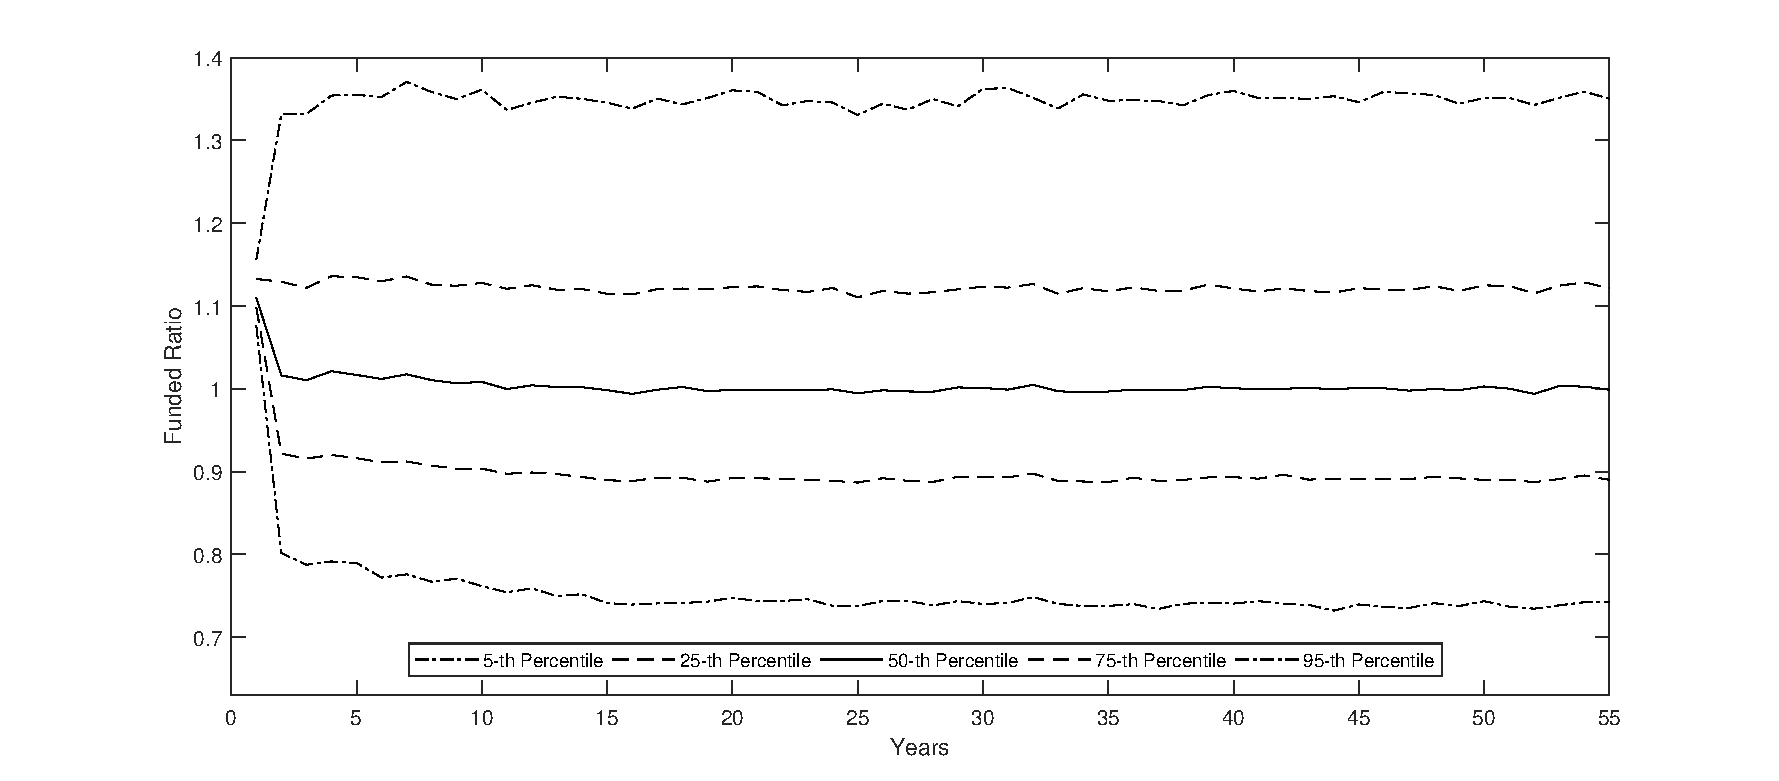
\includegraphics[width=1\linewidth]{ResultPlot/FR1.pdf} 
			\caption[Funnel of Doubt of Funded Ratio by Valuation Year in EROA Plan]{\textbf{Funnel of Doubt of Funded Ratio by Valuation Year in EROA Plan}
			\newline\footnotesize\justify The funded ratio of the plan before adjustment is calculated at each valuation date using Equation \eqref{eq:STBP_32}. The $5^{\text{th}}$, $25^{\text{th}}$, $50^{\text{th}}$, $75^{\text{th}}$ and $95^{\text{th}}$ percentiles of the simulated distribution of the funded ratio are shown in the plot.}
			\label{fig:Funnel of Doubt of Funded Ratio by Valuation Year in EROA Plan}
		\end{figure}
		\vspace{-0.4cm}
		\justify
		Figure \ref{fig:Value of the EROA Plan for All Cohorts} illustrates the value of the pension deal under this modified plan. In contrast to the negative pension value under the collective DC plan in Chapter \ref{Value-Based ALM Study of a Collective Defined Contribution Plan}, the members who are already retired at plan inception have a positive pension value when using EROA as the valuation rate. This is because their retirement benefits consume a portion the surplus from the initial contributions of both the active members and the retirees. Those who are still active at plan inception (i.e., retire after all the surplus is spent) are worse off because the surplus included in their initial contributions is paid out to the retirees and the probability of positive benefit adjustments is lower than under the collective DC plan. 
	
	
		\justify
	    Figure \ref{fig:Surplus and Deficit Options in EROA Plan} shows the value of the call and put options under the modified plan. The benefit options plot shows that the total value of the benefit call options is greater than the total value of the benefit puts for generations older than $58$ at plan inception. The values of $VTBC$ and $VTBP$ are both slightly lower than under the collective DC plan, which indicates less potential for inter-generational subsidies in the modified plan. The value of the residual call option under the modified plan is reduced to half of that under the collective DC plan, but it is still higher than the value of the residual put. This residual value can be due to several reasons. Most importantly, the EROA is an estimate calculated by adding a constant equity risk premium to the long-term bond yield, thus it is not perfectly lined up with the distribution of the actual asset returns, potentially giving rise to residual savings at the termination of the plan.
    
    
    	\begin{figure}[H]
			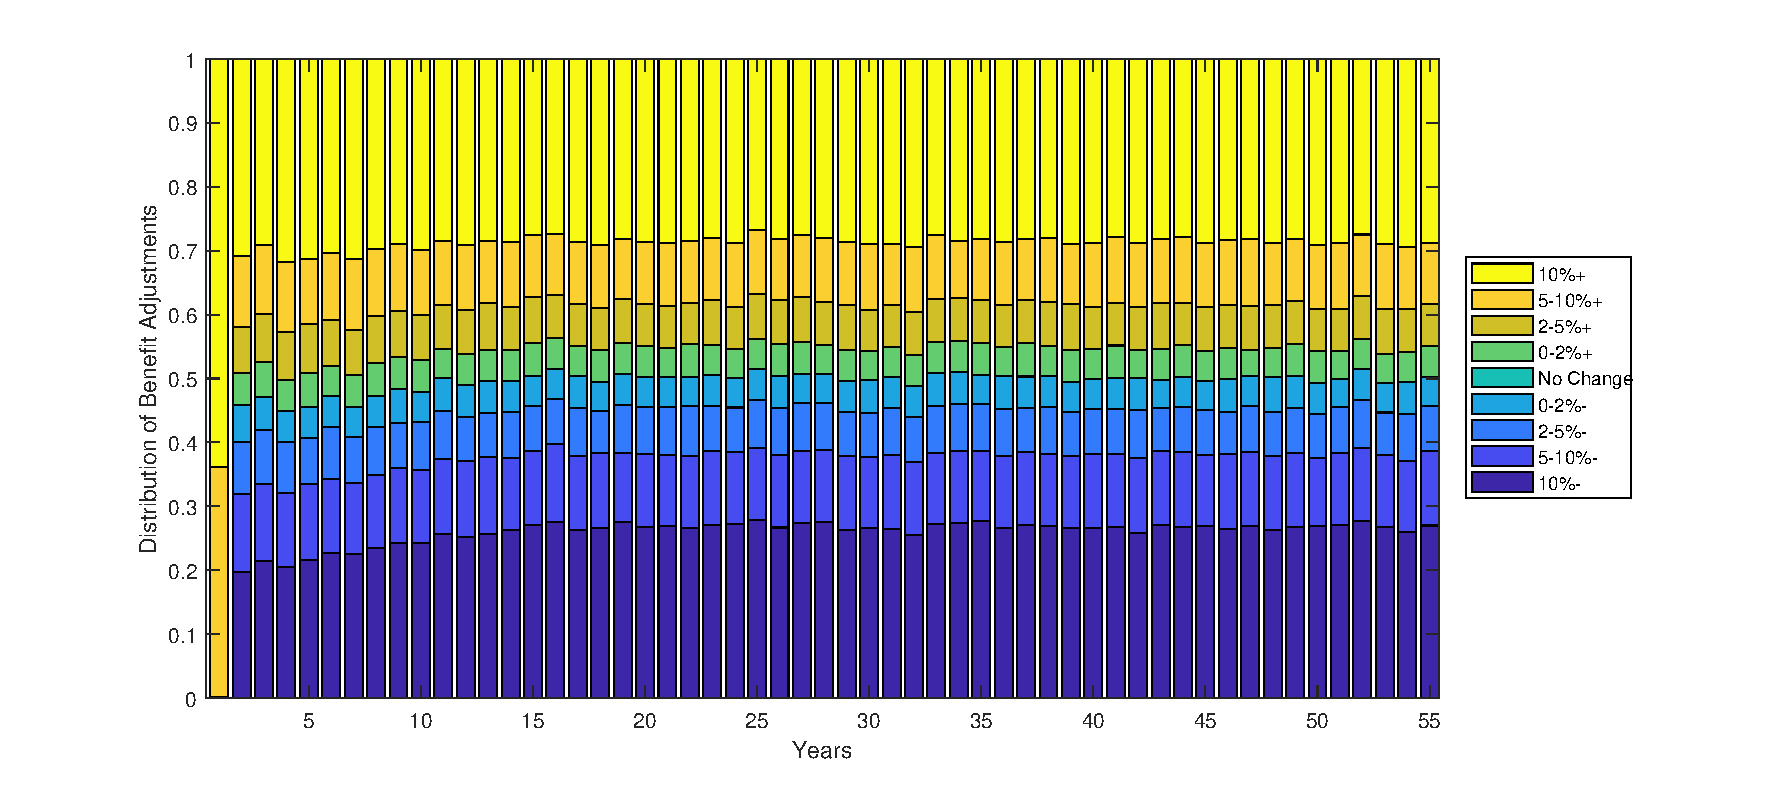
\includegraphics[width=1\linewidth]{ResultPlot/ProbIncDc1.pdf} 
			\caption[Distribution of Benefit Adjustments by Valuation Year]{\textbf{Distribution of Benefit Adjustments by Valuation Year}
			\newline\footnotesize\justify See Figure \ref{fig:Distribution of Benefit Adjustments by Valuation Year}.}
			\label{fig:Distribution of Benefit Adjustments by Valuation Year 2}	
		\end{figure}
		\vspace{-0.3cm}
		\begin{figure}[h]
			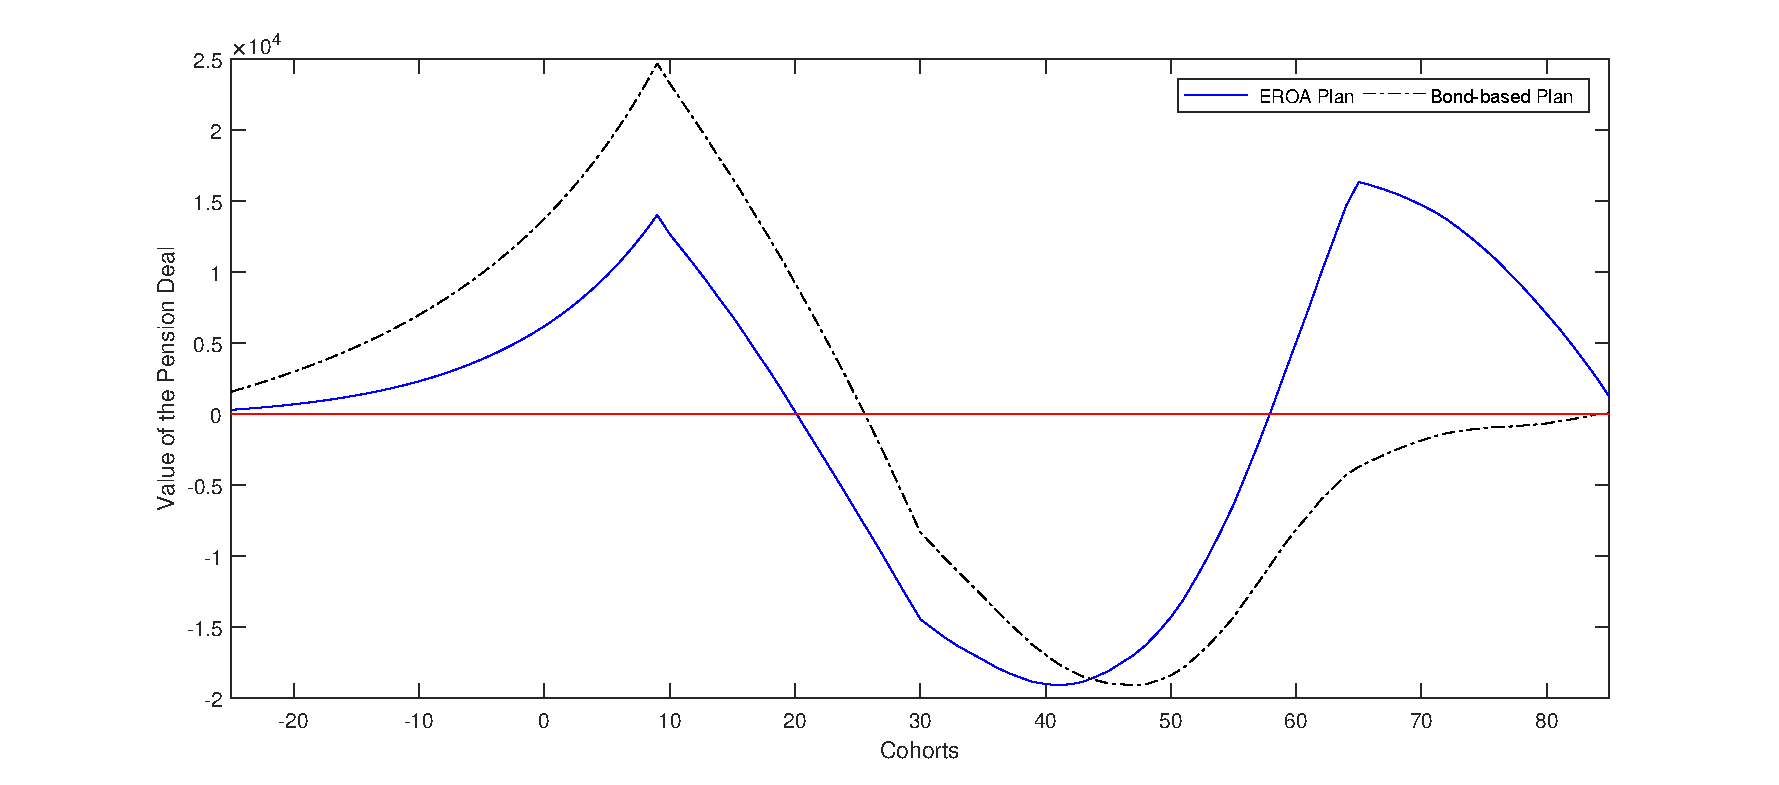
\includegraphics[width=1\linewidth]{ResultPlot/VPension1.pdf} 
			\caption[Value of the EROA Plan and Bond-based Collective DC Plan for All Cohorts]{\textbf{Value of the EROA Plan and Bond-based Collective DC Plan for All Cohorts}
			\vspace{-0.4cm}
			\newline\footnotesize\justify See Figure \ref{fig:Value of the CDC Plan for All Cohorts}. The solid line represents the generational values under the EROA plan and the dashed line represents the generational values under the collective DC plan with bond-based valuation rate.}
			\label{fig:Value of the EROA Plan for All Cohorts}
		\end{figure}
	
	
		\begin{figure}[H]
			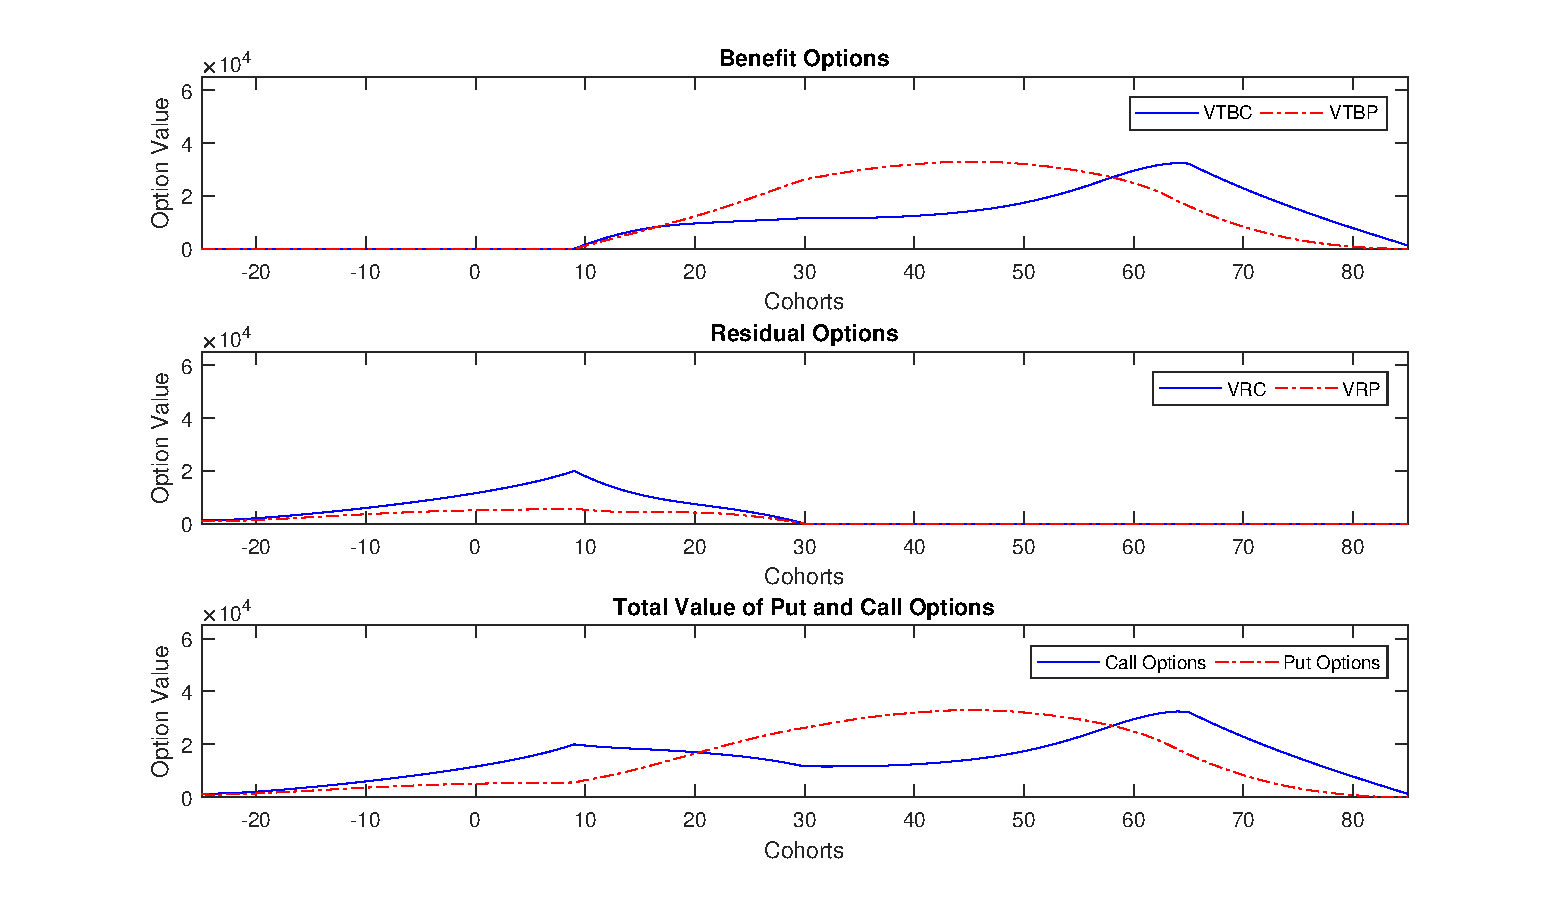
\includegraphics[width=1\linewidth]{ResultPlot/SDOptions1.pdf} 
			\caption[Embedded Options in EROA Plan Relative to Individual DC Benchmark]{\textbf{Embedded Options in EROA Plan Relative to Individual DC Benchmark}
			\newline\footnotesize\justify See Figure \ref{fig:Surplus and Deficit Options}.}
			\label{fig:Surplus and Deficit Options in EROA Plan}
		\end{figure}
       \begin{figure}[H]	
			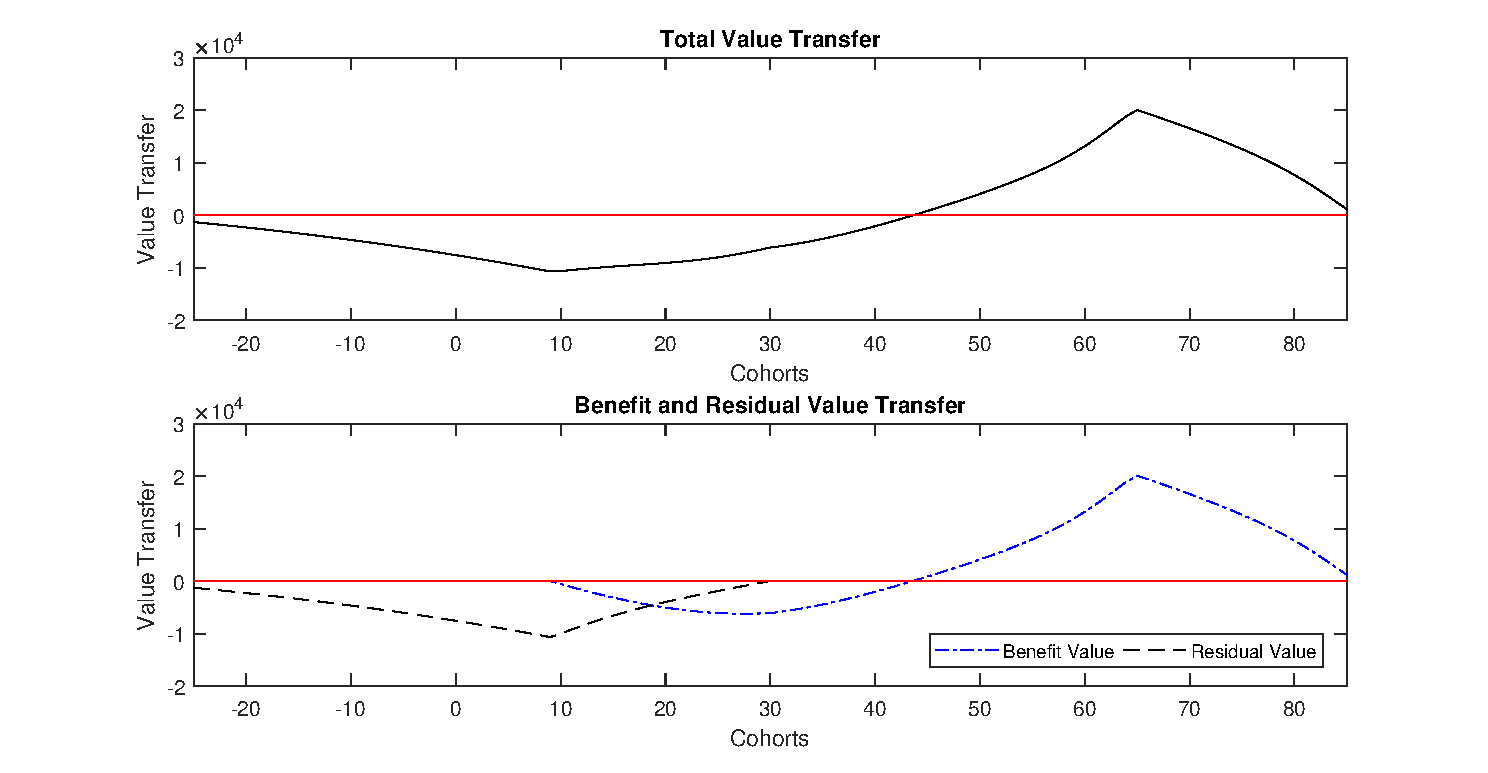
\includegraphics[width=1\linewidth]{ResultPlot/Vtrans1.pdf} 
			\caption[Value Transfers Caused by Changing Valuation Basis]{\textbf{Value Transfers Caused by Changing Valuation Basis}
			\vspace{-0.4cm}
			\newline\footnotesize\justify The figure on the top shows the total value transfers due to changing the valuation basis from a bond-based valuation rate to a EROA. The figure at the bottom separates the value transfers due to the benefit options versus the residual options.}
			\label{fig:Value Transfers Caused by Changing Valuation Rate}
		\end{figure}
	
		\vspace{-0.4cm}
		
		\justify
		Figure \ref{fig:Value Transfers Caused by Changing Valuation Rate} isolates the value transfers (that is, the changes in the value of the pension deal) due to changing the valuation basis. Overall, the values are shifted from the younger generations to those over age $45$ at inception. Most of the benefit gains for older generations come from the loss of residual value for younger generations. This is consistent with the fact that the EROA as valuation rate would decrease the plan liability and increase the funded ratio early on, accelerate the payment of larger benefits, and thus reduce the residual assets of the plan.
    
    
    	\justify
		In our findings, the difference between the retirement benefit dynamics in the EROA case and the bond-based case are consistent with Ma (2018). However, under our specific model and plan provisions, it is unclear whether using the EROA as valuation rate is ``more equitable''. In our model, using the EROA instead of a bond-based valuation rate simply shifts the expected residual benefits of future generations to retirees at plan inception. The generations who are $30$ to $50$ years old at plan inception still have a sizable expected net loss. To be truly ``more equitable'', this loss would need to be addressed. Simply switching the valuation basis does not achieve this.

	
	
	\section{TBP Designs with Different Triggers}
	\label{TBP Designs with Different Triggers}
	
		\justify
		The retirement benefits in the collective DC plan are adjusted at every valuation date and can fluctuate a lot. Plan designs with two triggers are adopted commonly in practice to add stability to the TBP. There may be a sense among TBP stakeholders that the benefit stability achieved by introducing the no-action range comes at no additional cost. The report of the CIA Task Force on Target Benefit Plans \citep{cia2015b} points out that this is made possible by requiring potentially larger inter-generational subsidies and draws attention to the associated risks. In this section, we investigate these subsidies, focusing on fairness \textit{ex ante}.
	
	
	\subsection{Triggers Centred at a Funded Ratio of $100\%$}
	\label{Triggers Centered at a Funded Ratio of 100}
	
		\justify
		Following \citet{Sanders2016a}, we first add a no-action range for funded ratios between $80\%$ and $120\%$ to the modified plan design from Section \ref{TBP Designs with Different Valuation Rate Assumption} (i.e., the collective DC plan using the EROA as the valuation rate). Since this range is centred around a funded ratio of $100\%$, this plan is called a symmetric corridor plan. Under this plan design, benefits are unchanged until the funded ratio moves outside the no-action range, at which point adjustments are made to bring the funded ratio closer to the edge of the range. For example, if the funded ratio is $140\%$ at the valuation date, then an adjustment factor $\alpha_{t}$ is applied to both the past and future accrual rates to bring the funded ratio close to $120\%$. Mathematically,
	     \begin{equation}
			\label{eq:CDTBP_1}
			\alpha_{t} = \frac{\frac{F_{t}}{120\%}+PVFNC_{t}}{PVTBP_{t} + PVTBF_{t}}.
	     \end{equation}
     
 	\vspace{-0.2cm}
     
     \justify
		Figure \ref{fig:Funnel of Doubt of the Funded Ratio by Valuation Year in Symmetric Corridor Plan} shows the funnel of doubt of the funded ratio under our symmetric corridor plan. The median of the funded ratio starts at a value higher than $100\%$ due to the lack of consistency between the initial target accrual rate of $1\%$ and the affordability test. However, unlike  the EROA case where the funded ratio is brought back towards $100\%$ immediately, the median funded ratio in the symmetric corridor plan drifts towards the centre of the no-action range slowly over time. We call the period while the distribution is shifting a transitional period. After about $15$ years, the distribution of the funded ratio becomes stationary. Note that in this symmetric corridor plan, the initial surplus is retained in the plan  instead of being paid out through large benefit increases in the early years. This surplus is then allowed to be eroded by negative plan experience (or boosted by positive plan experience, as the case may be).

		\begin{figure}[H]
			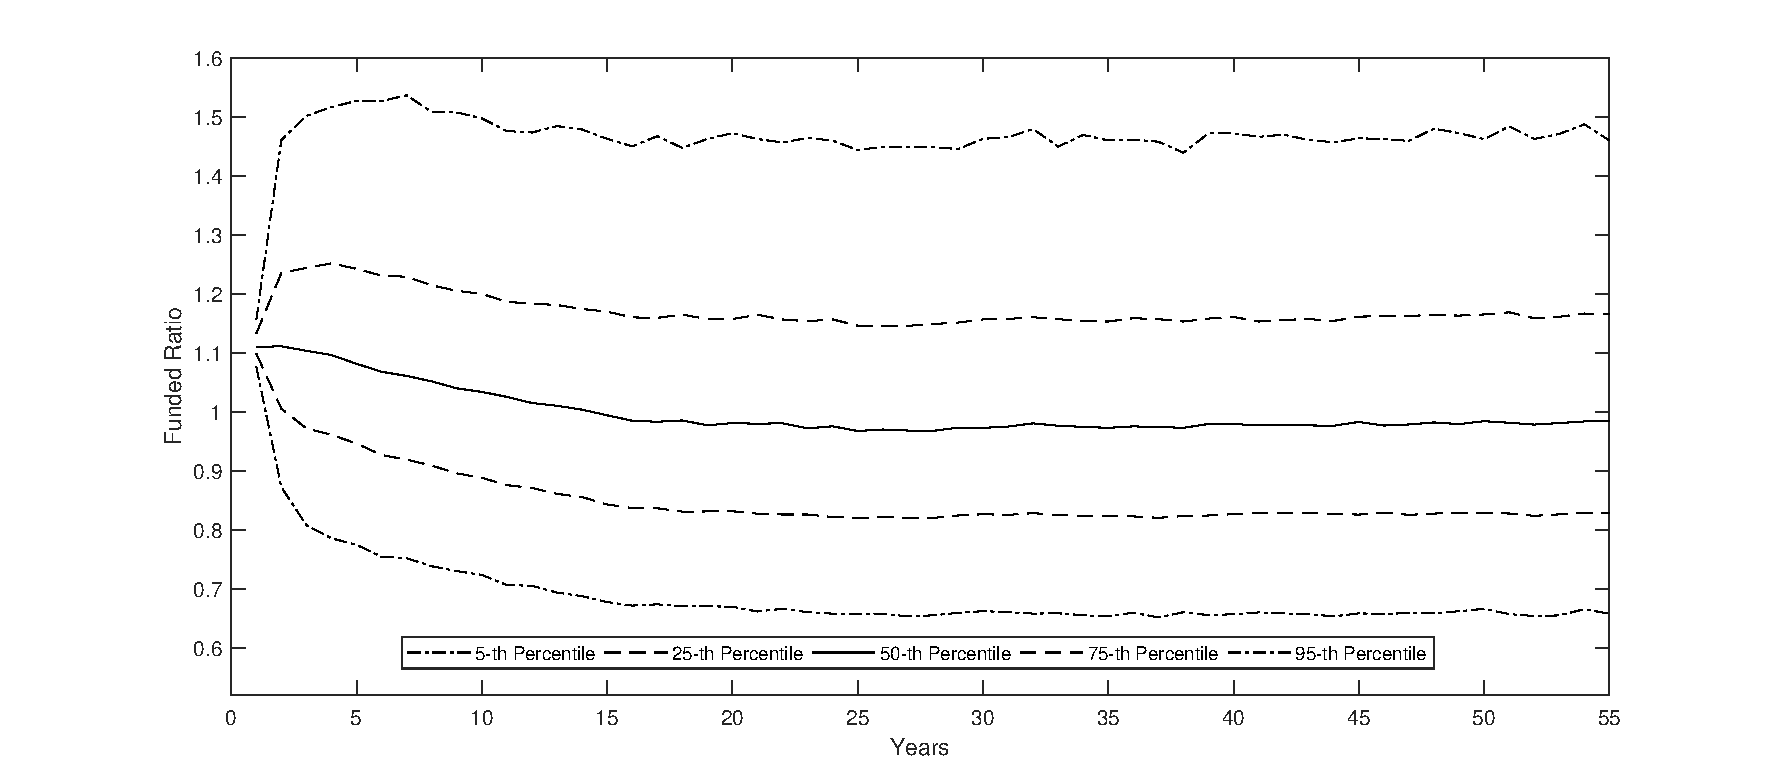
\includegraphics[width=1\linewidth]{ResultPlot/FR2.pdf} 
			\caption[Funnel of Doubt of the Funded Ratio by Valuation Year in Symmetric Corridor Plan]{\textbf{Funnel of Doubt of the Funded Ratio by Valuation Year in Symmetric Corridor Plan}
			\vspace{-0.4cm}
			\newline\footnotesize\justify See Figure \ref{fig:Funnel of Doubt of Funded Ratio by Valuation Year in EROA Plan}.}
			\label{fig:Funnel of Doubt of the Funded Ratio by Valuation Year in Symmetric Corridor Plan}	
		\end{figure}
		
		\begin{figure}[H]
			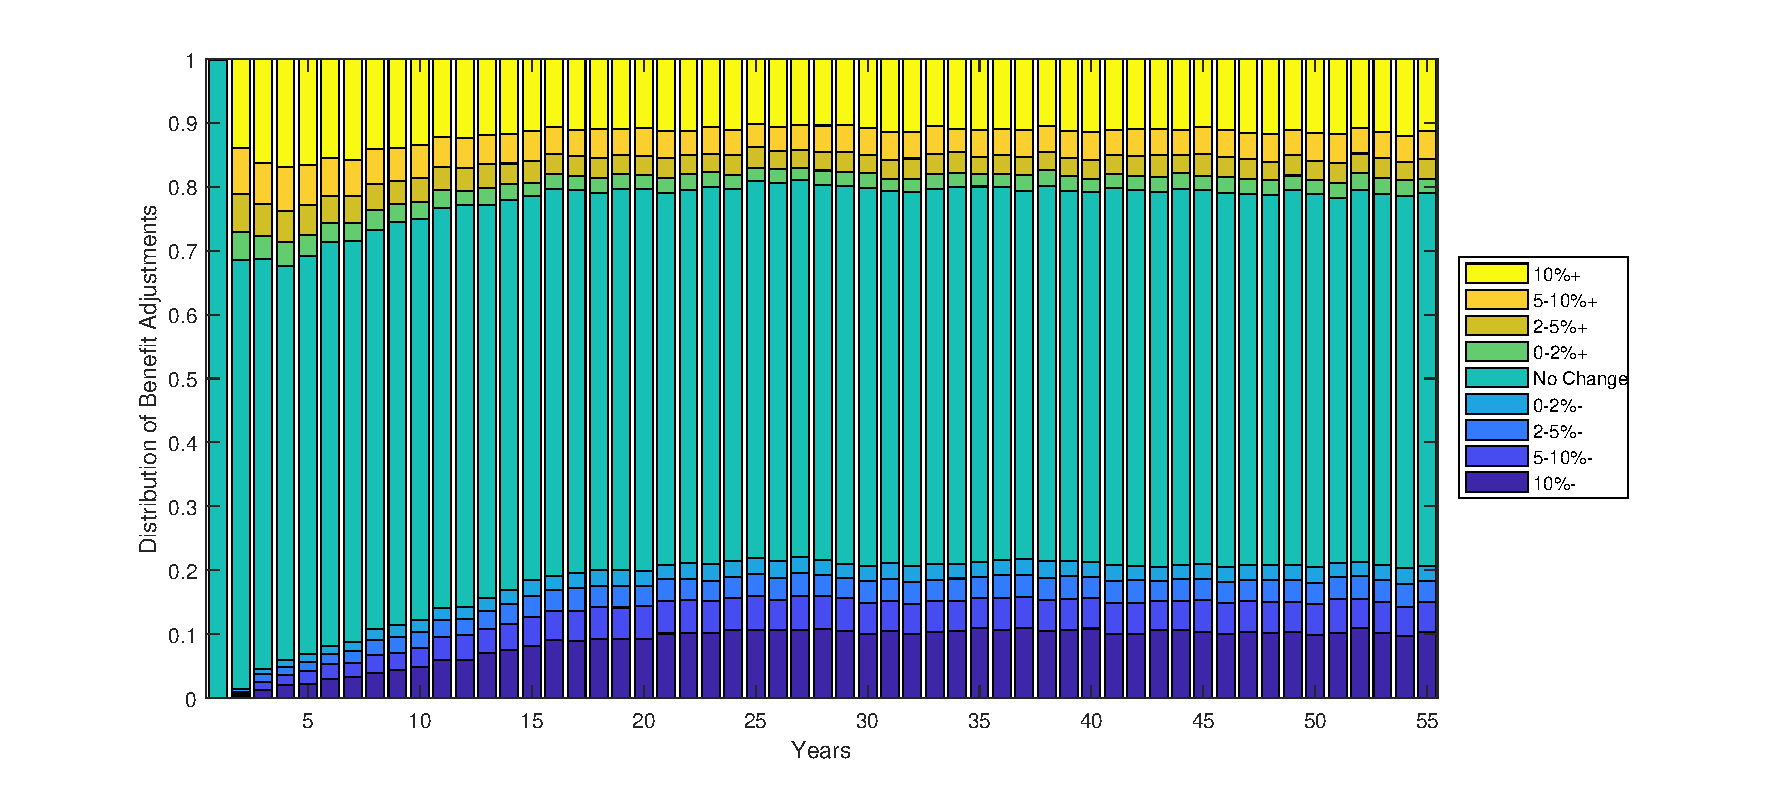
\includegraphics[width=1\linewidth]{ResultPlot/ProbIncDc2.pdf} 
			\caption[Distribution of Benefit Adjustments by Valuation Year]{\textbf{Distribution of Benefit Adjustments by Valuation Year}
			\vspace{-0.4cm}
			\newline\footnotesize\justify See Figure \ref{fig:Distribution of Benefit Adjustments by Valuation Year}.}
			\label{fig:Distribution of Benefit Adjustments by Valuation Year 3}
		\end{figure}

		\begin{figure}[H]
			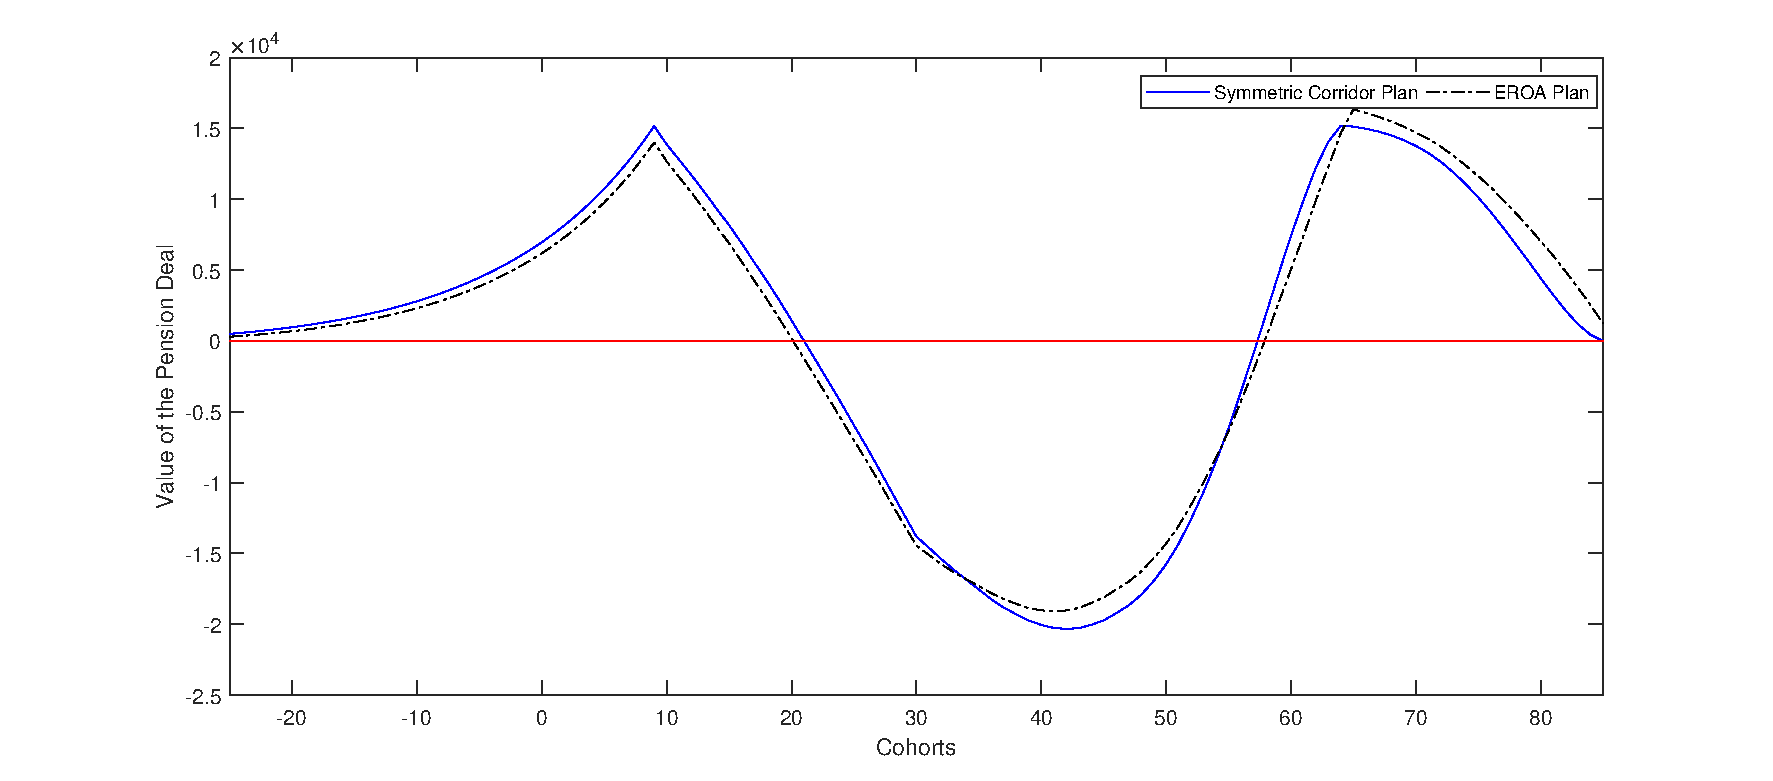
\includegraphics[width=1\linewidth]{ResultPlot/VPension2.pdf} 
			\caption[Value of the Symmetric Corridor Plan and the EROA Plan for All Cohorts]{\textbf{Value of the Symmetric Corridor Plan and the EROA Plan for All Cohorts}
			\newline\footnotesize\justify See Figure \ref{fig:Value of the CDC Plan for All Cohorts}. The solid line represents the generational values under the symmetric corridor plan and the dashed line represents the generational values under the EROA plan.}
			\label{fig:Value of the Symmetric Corridor Plan for All Cohorts}	
		\end{figure}
    	\begin{figure}[H]
			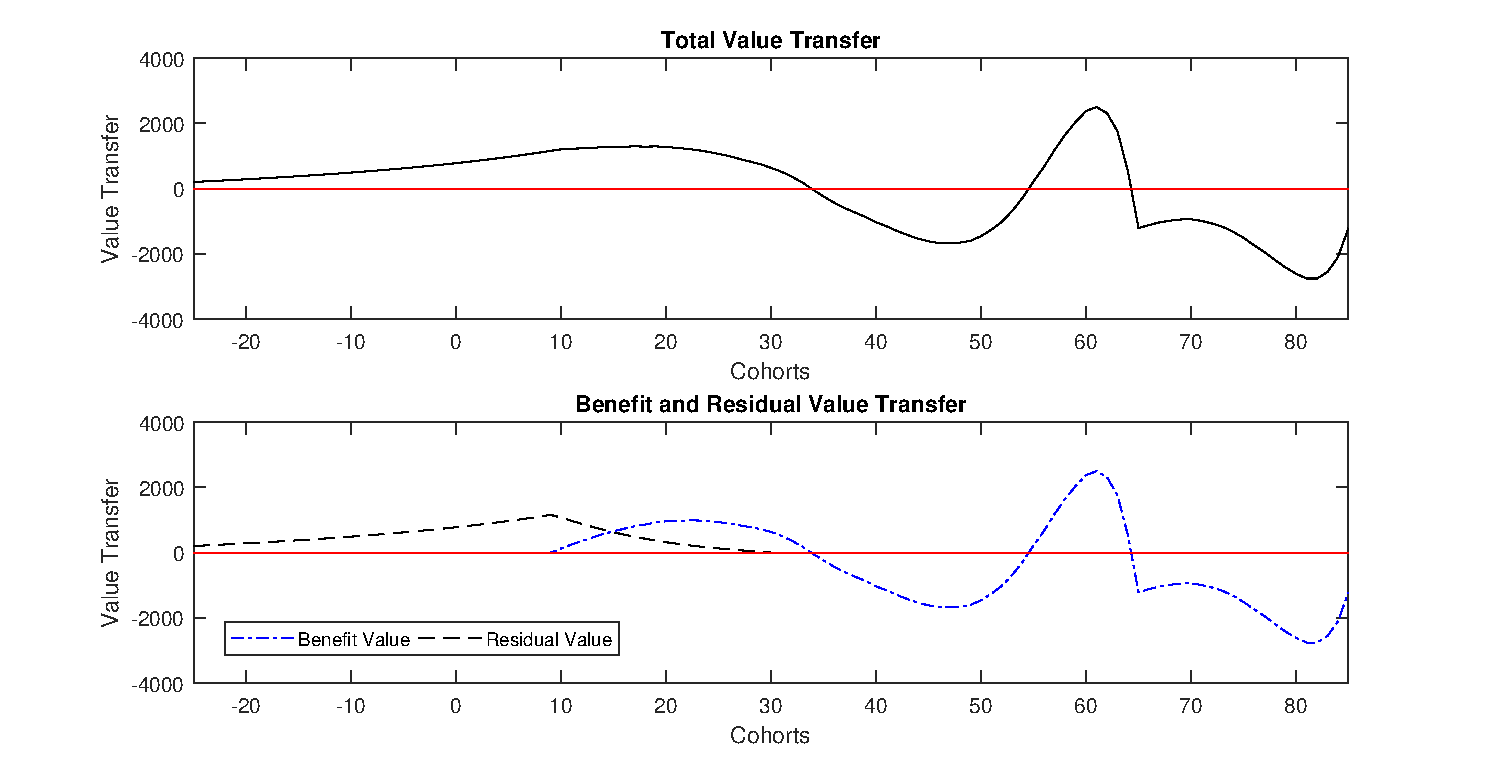
\includegraphics[width=1\linewidth]{ResultPlot/Vtrans2.pdf} 
			\caption[Value Transfers Created by Adding a Symmetric No-action Range]{\textbf{Value Transfers Created by Adding a Symmetric No-action Range}
			\vspace{-0.4cm}
			\newline\footnotesize\justify See Figure \ref{fig:Value Transfers Caused by Changing Valuation Rate}.}
			\label{fig:Value Transfers Created by Adding a Symmetric No-action Range}
		\end{figure}
		
		\justify
		The key advantage of the no-action range is that it reduces the frequency and magnitude of benefit changes. From Figure \ref{fig:Distribution of Benefit Adjustments by Valuation Year 3}, we can observe that the benefits remain the same from one year to another with more than $50\%$ probability, whereas the benefits are changed at every valuation date under the collective DC plans without no-action ranges. The probability of a large benefit adjustment (i.e., an increase or decrease greater than $10\%$) occurring in the first year is reduced to $20\%$ from over $50\%$ in the collective DC plan and its EROA variant. In addition, the plan starts with a funded ratio higher than $100\%$, so negative adjustments are less likely during the transitional period because the plan starts with a ``buffer'' already in place.		
	
	
		\justify
		Figure \ref{fig:Value of the Symmetric Corridor Plan for All Cohorts} shows the value of the pension deal under the symmetric corridor plan design and Figure \ref{fig:Value Transfers Created by Adding a Symmetric No-action Range} shows the value transfers caused by adding a no-action range to the EROA plan. We find that the no-action range adds significant stability to the plan without creating any significant value transfers in our case. These results depend on a stable demographic profile and the assumption that the simulation of the economic variables is started from the long-term equilibrium level. However, given the current low interest rate environment, it may not be reasonable to assume that the economic and demographic conditions remain stationary over the next $50$ years.
    
    
	\subsection{Triggers Centred at a Funded Ratio around $120\%$}
	\label{Triggers Centred at a Funded Ratio around 120}

	
	
		\justify
	    Canadian regulations for TBPs allow (and often require) the use of no-action ranges, although not ones centred at $100\%$. Generally, the regulations require the lower end of the no-action range to start at $100\%$. We also want to explore inter-generational equity under this more realistic plan design. In this section, we implement a plan with lower and upper trigger points set at funded ratios of $100\%$ and $140\%$, respectively. Since the no-action range is deliberately biased to saving, we call this a saving corridor plan. 
		
		\begin{figure}[H]
			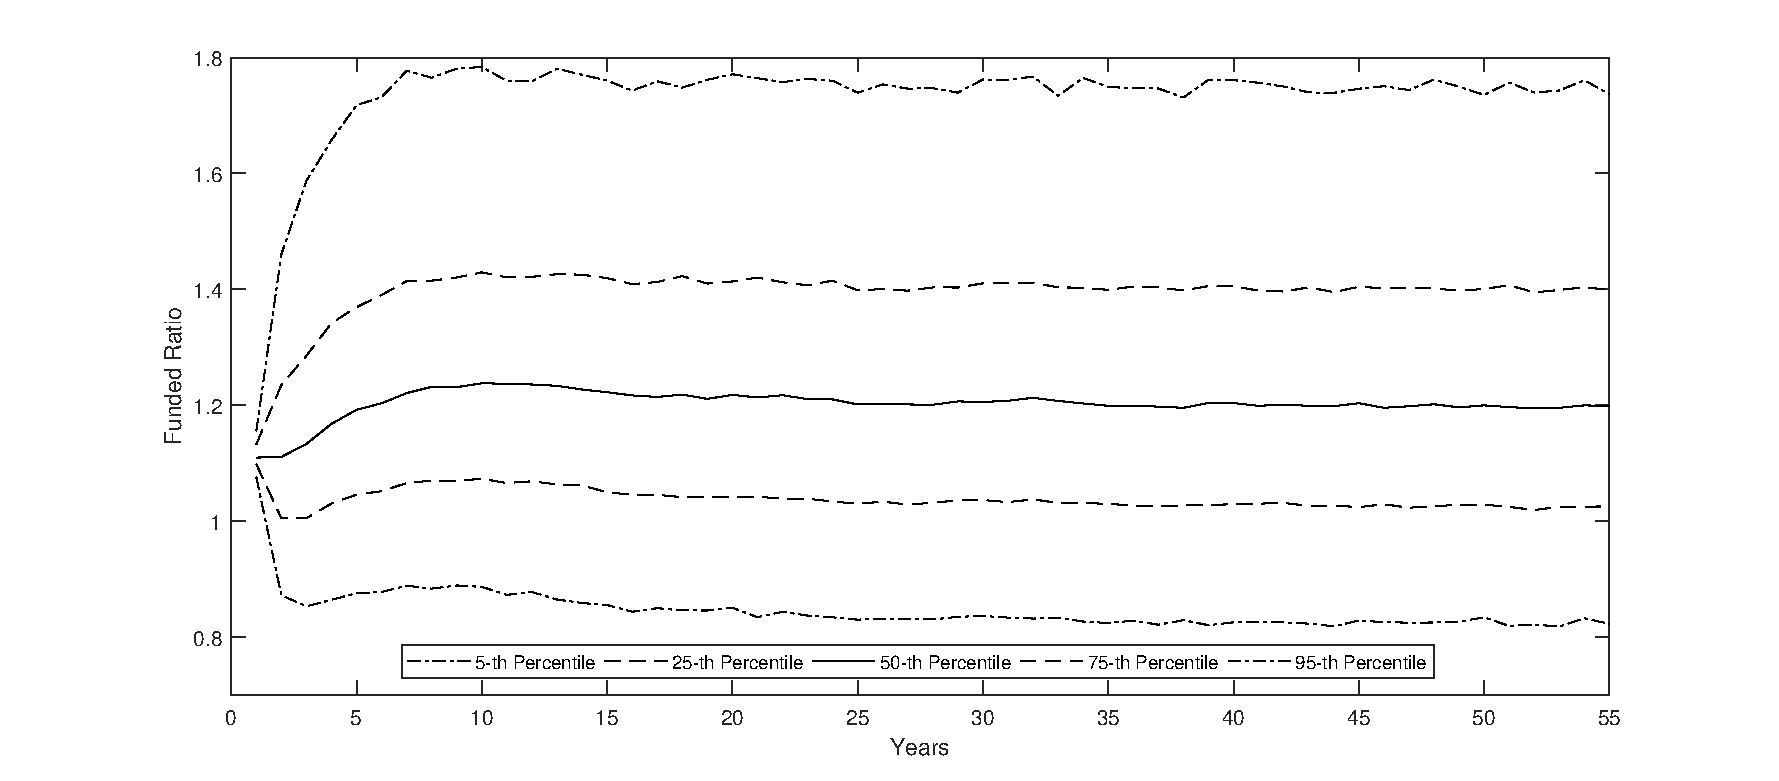
\includegraphics[width=1\linewidth]{ResultPlot/FR3.pdf} 
			\caption[Funnel of Doubt of Funded Ratio by Valuation Year in Saving Corridor Plan]{\textbf{Funnel of Doubt of Funded Ratio by Valuation Year in Saving Corridor Plan}
			\vspace{-0.4cm}
			\newline\footnotesize\justify See Figure \ref{fig:Funnel of Doubt of Funded Ratio by Valuation Year in EROA Plan}.}
			\label{fig:Funnel of Doubt of Funded Ratio by Valuation Year in Saving Corridor Plan}
		\end{figure}
	    
	    \justify
		The funnel of doubt of the funded ratio for the saving corridor plan is shown in Figure \ref{fig:Funnel of Doubt of Funded Ratio by Valuation Year in Saving Corridor Plan}. The first $10$ years form a transitional period during which time the distribution of the funded ratio widens and drifts upwards, from a value of $110\%$ at plan inception to the centre of the no-action range (i.e., 120\%). With the same $110\%$ initial funded ratio, the ``transitional period'' of the saving corridor plan corresponds to a process that tends to build up additional buffers, compared to a process that tends to erode the surplus in the symmetric corridor plan. As a result, the benefits are less likely to be adjusted upward and more likely to be adjusted downward than under the symmetric corridor plan, at least in the early years. This is confirmed in Figure \ref{fig:Distribution of Benefit Adjustments by Valuation Year 4}. After the first $10$ years, the probability of the benefits remaining unchanged in a given valuation is around $50\%$, which is the same as under the symmetric corridor plan. This is because the no-action ranges have the same ``size'' or ``span'' in terms of the funded ratio. However, the probability of positive benefit adjustments is slightly higher and the probability of negative benefit adjustments is slightly lower under the saving corridor plan than under the symmetric corridor plan because of more savings in the early years of plan operations.
		
		\begin{figure}[H]
			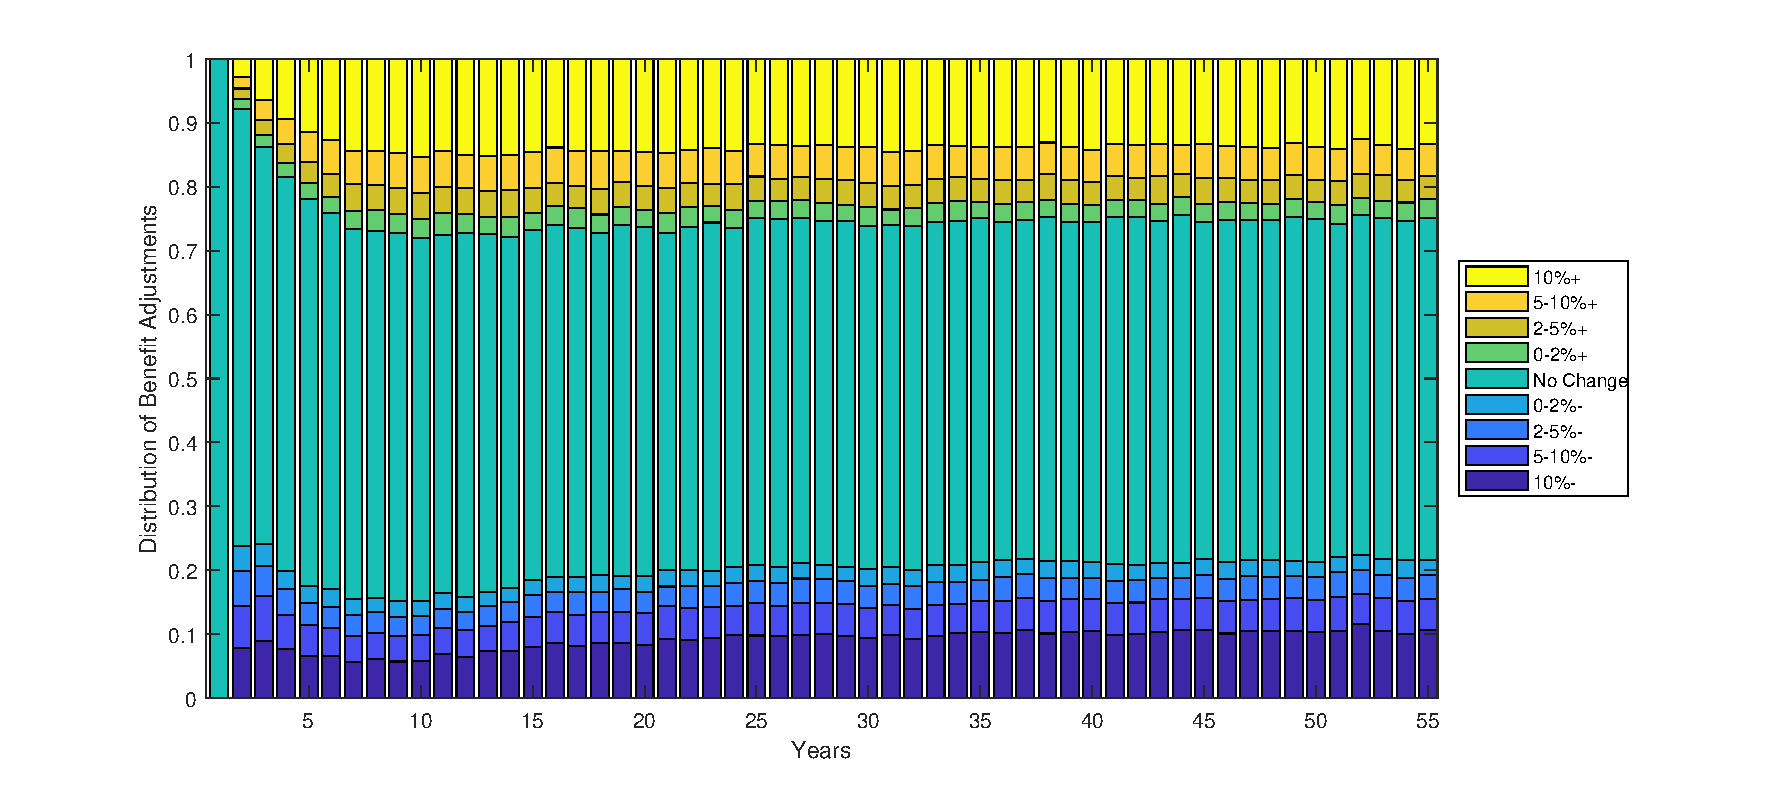
\includegraphics[width=1\linewidth]{ResultPlot/ProbIncDc3.pdf} 
			\caption[Distribution of Benefit Adjustments by Valuation Year]{\textbf{Distribution of Benefit Adjustments by Valuation Year}
			\vspace{-0.4cm}
			\newline\footnotesize\justify See Figure \ref{fig:Distribution of Benefit Adjustments by Valuation Year}.}
			\label{fig:Distribution of Benefit Adjustments by Valuation Year 4}
		\end{figure}
	
	
		\begin{figure}[h]
			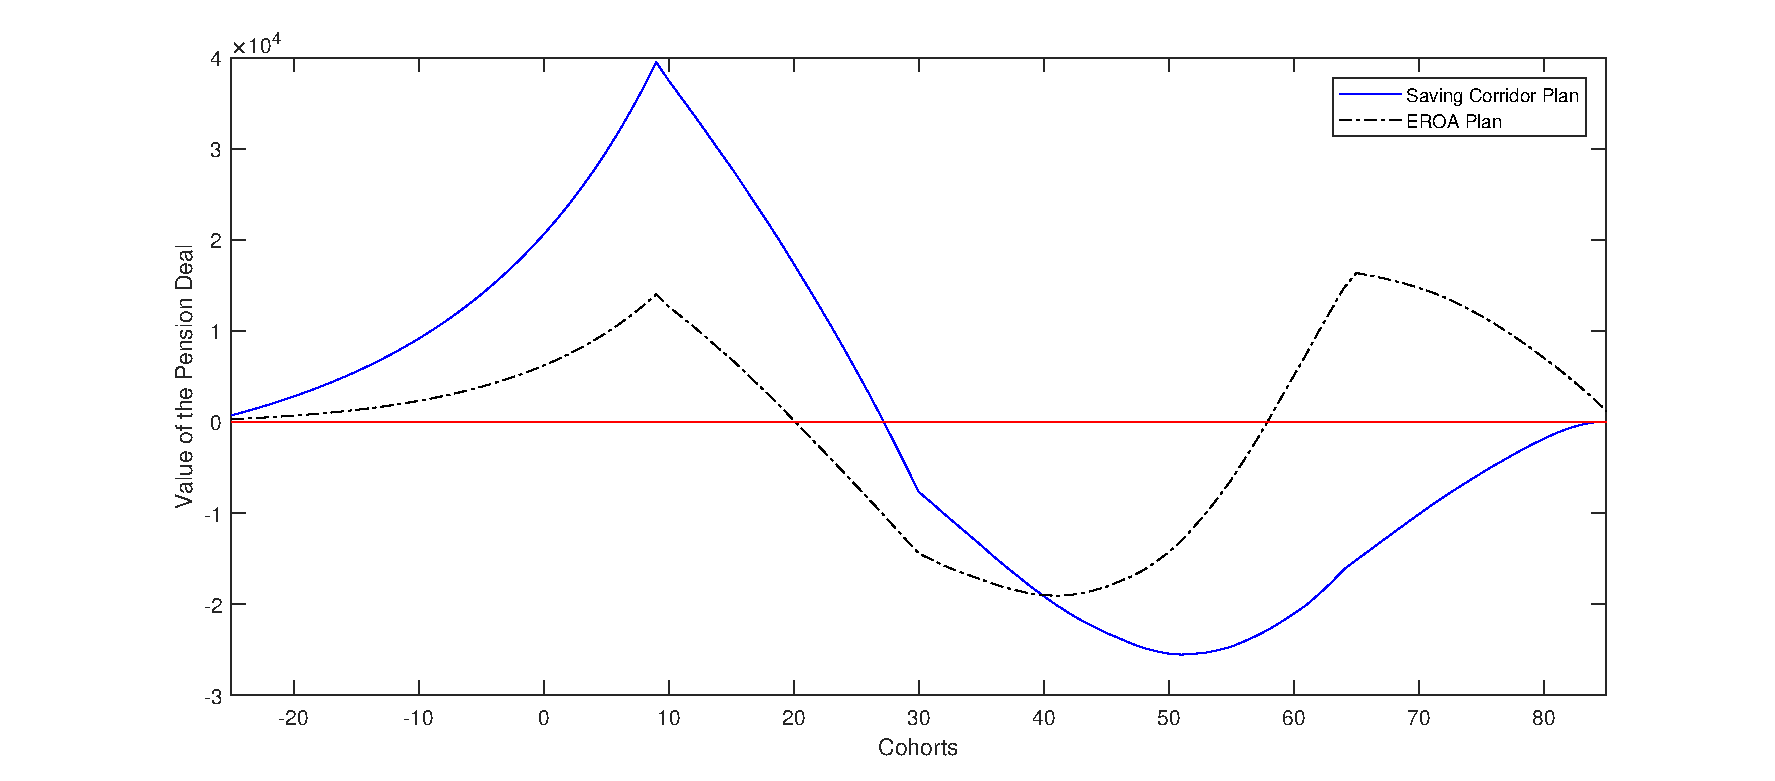
\includegraphics[width=1\linewidth]{ResultPlot/VPension3.pdf} 
			\caption[Value of the Saving Corridor Plan and EROA Plan for All Cohorts]{\textbf{Value of the Saving Corridor Plan and EROA Plan for All Cohorts}
			\newline\footnotesize\justify See Figure \ref{fig:Value of the CDC Plan for All Cohorts}. The solid line represents the generational values under the saving corridor plan and the dashed line represents the generational values under the EROA plan.}
			\label{fig:Value of the saving Corridor Plan for All Cohorts}
		\end{figure}
		\vspace{-0.4cm}
		
		\justify
		Figure \ref{fig:Value of the saving Corridor Plan for All Cohorts} illustrates the  value of the pension deal under the saving corridor plan design. Under this plan design, all generations younger than age $30$ have positive plan values because the median size of the buffer held by the plan is equal to about $20\%$ of the total liabilities. When the plan is terminated, any extra savings will be distributed to the generations that remain in the plan at that time. This is similar to distributing the extra savings accumulated under the collective DC plan with a bond-based (conservative) valuation rate, except that the size of the extra savings here is larger than under the collective DC plan in Chapter \ref{Value-Based ALM Study of a Collective Defined Contribution Plan}. All generations who are not entitled to this residual surplus at plan termination are worse off under this design because part of the plan benefits tend to be held back to build the extra buffer. 

		\begin{figure}[h]
			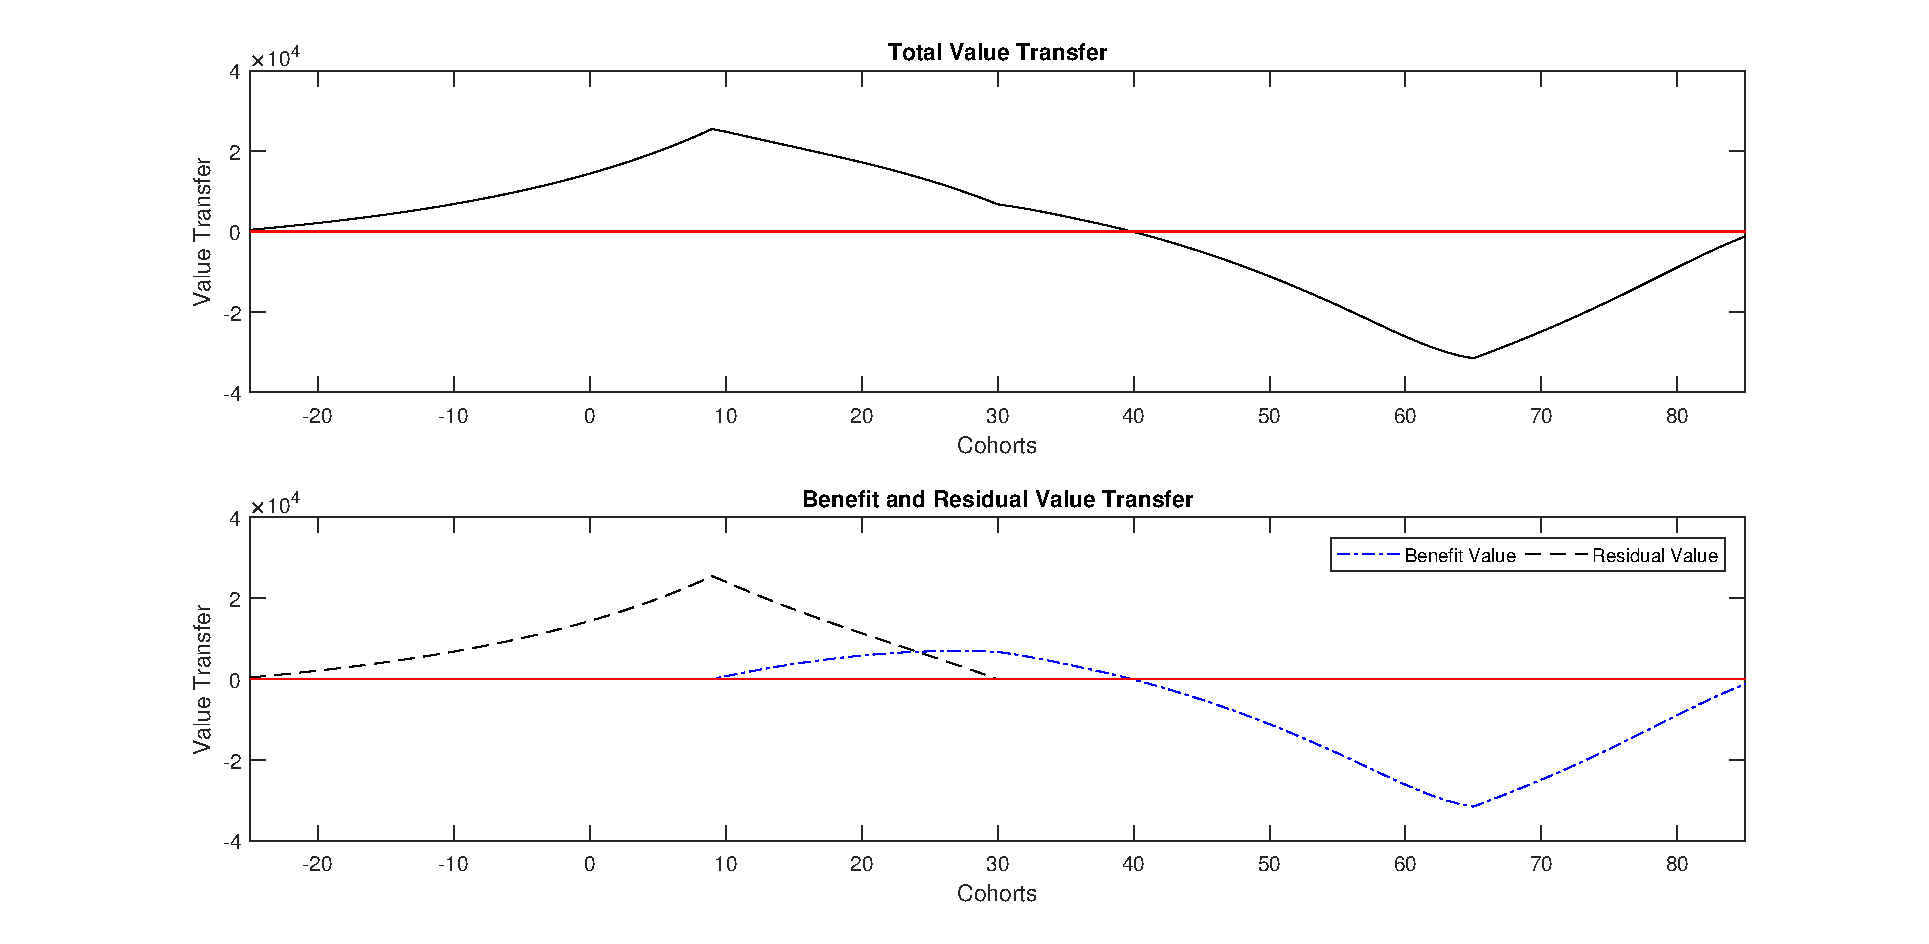
\includegraphics[width=1\linewidth]{ResultPlot/Vtrans3.pdf} 
			\caption[Value Transfers Created by Adding a Saving Biased No-action Range]{\textbf{Value Transfers Created by Adding a Saving Biased No-action Range}
			\vspace{-0.4cm}
			\newline\footnotesize\justify See Figure \ref{fig:Value Transfers Caused by Changing Valuation Rate}.}
			\label{fig:Value Transfers Created by Adding a Saving Biased No-action Range}
		\end{figure}

	
		\justify
		Figure \ref{fig:Value Transfers Created by Adding a Saving Biased No-action Range} shows the value transfers resulting from shifting the no-action range up from $(80\%, 120\%)$ to $(100\%, 140\%)$. There is a clear shift in value from older cohorts to younger cohorts. The oldest active cohort at plan termination, who is $9$ years old at plan inception, is expected to have the largest gain under this plan design equal to nearly $\$40\text{,}000$ in terms of market-consistent value. This generation has the highest actuarial liability at plan termination, thus is expected to share the largest portion of the extra savings in the residual assets. The generation retiring right after plan inception has the largest loss (around $\$30\text{,}000$), equivalent to nearly $60\%$ of their final year earnings. This is because a part of the surplus which would otherwise fund benefit increases is retained in the plan for building up a larger buffer. From these results, we can conclude that the stability under the saving corridor plan does come at someone's expense: in this case, at the expense of older generations. 
	
		\justify
		An interesting fact is that the cohorts between 30 and 55 years old at plan inception have negative pension values under all of the four plan designs. The initial account values brought into the plan at inception are more than enough to cover the plan liabilities, if the plan uses the EROA as the valuation rate. However, all the resulting surplus is paid out during the first few years of plan's operations, benefiting mostly the generations who are already retired or close to retirement. The generations that retire later, i.e., younger than $55$ years old at plan inception, are not expected to get back their portion of the initial surplus. Under plan designs that are biased towards saving---such as the collective DC plan in Chapter \ref{Value-Based ALM Study of a Collective Defined Contribution Plan} and the saving corridor plan---all the generations who retire while the plan is ongoing lose value because part of their benefits are retained in the fund for future generations. These extra savings are expected to be paid out at plan termination through the distribution of residual assets. The cohorts who are older than $30$ have no entitlement to the residual assets, therefore their savings are passed on to the younger generations. 
	
	
	\chapter{Conclusion}
	\label{Conclusion}

		\justify
		In this research, we study inter-generational equity under different TBP designs using the value-based ALM framework. We investigate the wealth redistribution effect of changing key plan design elements, such as changing valuation assumptions and adding different benefit stability mechanisms. The operations of four target benefit plans are studied using Monte Carlo simulation over a 55-year time horizon. The complex cash flows in respect of different generations are recorded separately using the generational accounting technique. The contingent retirement benefits paid under each plan are formulated as combinations of several embedded options written between the pension fund and the plan members. The value of the pension deal for each generation is evaluated using the risk-neutral asset pricing technique and compared across different plan designs. To generate the economic scenarios on which the future evolution of pension funds depends, a real-world VAR-GARCH model is constructed. In addition, a corresponding risk-neutral model is derived and calibrated to help with the pricing of the embedded options within the pension contract.
	
		\justify
		The first of the four TBP designs studied in this research is a basic collective DC plan with a bond-based valuation rate. In the second plan, the bond-based valuation rate is replaced with the expected return on assets. Lastly, we study two plans with benefit stabilizing designs, including the so-called symmetric corridor plan and the saving corridor plan. 
	
	
		\justify
		For each plan, annual valuations are performed using the EAN method. Both past and future accrual rates are adjusted simultaneously at each valuation date based on the plan's funded position. Plan costs are held constant---same initial asset and contribution rate---to ensure the retirement benefits under various plan designs are comparable. 
	
	
		\justify
		By comparing the generational value of the pension deal under these plan designs, we find that:
		\begin{itemize}
			\item Value transfers arise by simply joining the collective pension scheme even without the inclusion of any intertemporal benefit smoothing designs, because the inflation and valuation rate risks are  shared implicitly among different generations.
			\item TBPs with designs that are biased to saving, i.e., the saving corridor plan and the collective DC plan with bond-based valuation rate, tend to shift value from older generations to younger generations, who  are entitled to the residual assets of the fund at plan termination.
			\item Changing the valuation rate from the bond-based rate to the EROA transfers part of the surplus of younger generations to the generations who already retired or are close to retirement at plan inception, but is not able to improve the inter-generational equity in our case.
			\item Adding a symmetric corridor can reduce the volatility of retirement benefits without triggering significant value transfers, at least under the assumption of stationary demographic profile and when the simulation of economic scenarios starts from its long-term equilibrium level.
			\item Generations aged between 30 to 55 are expected to lose value under all four plan designs due to how the initial contribution rate is set and how the residual assets are distributed at plan termination.
		\end{itemize}
	
	
		\justify
		All of our results are conditional on the assumptions that the simulation of the economic scenarios starts from its long-term equilibrium level and that the demographic experience is stationary with the number of new entrants equal to the number of people retiring in any given year. 
	
	
		\justify
	   In future research, the following directions could be investigated:
	   \begin{itemize}
	   	\item Starting the simulation of economic scenarios with different starting values (i.e., different from the equilibrium position).
	   	\item Investigating the inter-generational value transfers of the TBPs under non-stationary demographic structures.
	   	\item Adding the stochastic mortality to the liability model of the pension plan.
	   	\item Investigating the generational impact of changing valuation method in the affordability test, such as using the Projected Unit Credit method which is commonly used in practice.
	   	\item Developing new valuation method and new action rules that can improve the fairness of the TBP.
	   	\item Testing the inter-generational equity under different TBP designs from the \textit{ex post} perspective.	   	
	   \end{itemize}

	
	
	
	
	%   BACK MATTER  %%%%%%%%%%%%%%%%%%%%%%%%%%%%%%%%%%%%%%%%%%%%%%%%%%%%%%%%%%%%%%
	%
	%   References and appendices. Appendices come after the bibliography and
	%   should be in the order that they are referred to in the text.
	%
	%   If you include figures, etc. in an appendix, be sure to use
	%
	%       \caption[]{...}
	%
	%   to make sure they are not listed in the List of Figures.
	%

		%\justify
		% Test for citation
		% \citet{Ahlgrim2008} \citet{Aitken1996} \citet{AonHewitt2015a} \citet{AonHewitt2015b}
		% \citet{AonHewitt2015c} \citet{AonHewitt2015d} \citet{Beetsma2014} \citet{Blake2001}
		% \citet{Hoevenaars2008} \citet{Ma2016} \citet{MacDonald2007} \citet{Reinsel1997}
		% \citet{Sanders2010} \citet{Sanders2014} \citet{Sanders2016a} \citet{Sanders2016b}
		% \citet{Sanders2016c} \citet{Settergren2001} \citet{Tsay2013} \citet{Wesbroom2013}
		% \citet{Wilkie1984} \citet{Wilkie1995} \citet{Ang2003} \citet{BOC} \citet{Blake2003}
		% \citet{Blommestein2009} \citet{Bovenberg2007} \citet{Broadbent2006} \citet{Brown2014}
	
	
	\backmatter%
	\addtoToC{Bibliography}
	\bibliographystyle{apa} %ksfh_nat
	\bibliography{references}
	
	
	% \begin{appendices} % optional
	% 	\chapter{Code}
	% \end{appendices}
\end{document}

% \begin{equation}
% \notag
% \begin{split}
%   &\boldsymbol{GA^{s}}=\\
%   &\begin{bmatrix}
%   0\\
%   0\\
%   \vdots\\
%   0\\
%   0\\
%   AVDC_{31,0}\\
%   \vdots\\
%   AVDC_{64,0}\\
%   AVDC_{65,0}\\
%   \vdots\\
%   AVDC_{84,0}\\
%   AVDC_{85,0}\\  
%   \end{bmatrix}
%   +
%   \begin{bmatrix}
%     0 		      &0             &0             &\cdots & 0             &0             &\cdots  &0 			   &C_{30,55}^{s}    \\
%     0  			  &0 			 &0  			&\cdots & 0 		  	&0 			   &\cdots  &C_{30,54}^{s} &C_{31,55}^{s}    \\
%     \vdots 		  &\vdots 		 &\vdots  	    &       & \vdots 	    &\vdots 	   &        &\vdots 	   &\vdots           \\
%     0  			  &C_{30,1}^{s}  &C_{31,2}^{s}  &\cdots & C_{63,34}^{s} &C_{64,35}^{s} &\cdots  &B_{83,54}^{s} &B_{84,55}^{s}    \\
%     C_{30,0}^{s}  &C_{31,1}^{s}  &C_{32,2}^{s}  &\cdots & C_{64,34}^{s} &B_{65,35}^{s} &\cdots  &B_{84,54}^{s} &B_{85,55}^{s}    \\
%     C_{31,0}^{s}  &C_{32,1}^{s}  &C_{33,2}^{s}  &\cdots & B_{65,35}^{s} &B_{66,55}^{s} &\cdots  &B_{85,54}^{s} &0                \\	
%     \vdots 		  &\vdots 		 &\vdots  	    &       & \vdots 	    &\vdots 	   &        &\vdots 	   &\vdots           \\
%     C_{64,0}^{s}  &B_{65,1}^{s}  &B_{66,2}^{s}  &\cdots & 0 		    &0 			   &\cdots  &0 			   &0                \\
%     B_{65,0}^{s}  &B_{66,1}^{s}  &B_{67,2}^{s}  &\cdots & 0 			&0 			   &\cdots  &0             &0                \\
%     \vdots 		  &\vdots 		 &\vdots  	    &       & \vdots 	    &\vdots 	   &        &\vdots 	   &\vdots           \\
%     B_{84,0}^{s}  &0             &0  			&\cdots & 0 			&0             &\cdots  &0             &0                \\
%     B_{85,0}^{s}  &0             &0  			&\cdots & 0 			&0             &\cdots  &0             &0                \\
%   \end{bmatrix}
%   +
%   \begin{bmatrix}
%   RV_{30,55}^s\\
%   RV_{31,55}^s\\
%   \vdots\\
%   RV_{84,55}^s\\
%   0\\
%   0\\
%   \vdots\\
%   0\\
%   0\\
%   \vdots\\
%   0\\
%   0\\  
%   \end{bmatrix}.
% \end{split}
% \end{equation}

